\documentclass[spanish]{book}
\usepackage{titlesec}

%Quitar páginas en blanco
\let\cleardoublepage\clearpage
\usepackage{etoolbox}
\makeatletter
\patchcmd{\@endpart}{\vfil\newpage}{\par}{}{}
\makeatother

%\usepackage[spanish]{babel} ¡Esto estaba interfiriendo con las flechitas de los \tikspicture

\renewcommand{\contentsname}{Índice}
\renewcommand{\partname}{Parte}

\titleformat{\chapter}[display]
{\normalfont\huge\bfseries}{}{0pt}{\Huge\thechapter.~}

\titleformat{name=\chapter,numberless}[display]
{\normalfont\huge\bfseries}{}{0pt}{\Huge}
\renewcommand{\chaptermark}[1]{\markboth{{} \thechapter: #1}{}}


%Cambiar el formato de los capítulos
\usepackage{titlesec}
\titleformat{\chapter}[display]
{\normalfont\huge\bfseries}{}{0pt}{\Huge\thechapter.~}
\titleformat{name=\chapter,numberless}[display]
{\normalfont\huge\bfseries}{}{0pt}{\Huge}
\renewcommand{\chaptermark}[1]{\markboth{{} \thechapter: #1}{}}

%Paquetes
\usepackage[left=4cm, right=4cm]{geometry}
\usepackage{palatino}%Fuente
\usepackage{graphicx}%Imágenes
\usepackage{float}%Imágenes
\usepackage{subcaption}%Imágenes
\usepackage{enumitem}%Listas
\usepackage{parskip}%Espacio entre párrafos
\usepackage{multicol}
\usepackage{amsthm}%Mate
\usepackage{amssymb}%Mate
\usepackage{amsmath}%Mate
\usepackage{mathtools}
\usepackage{tikz}%Mate (diagramas)
\usepackage{tikz-cd}
\usetikzlibrary{%
	matrix,%
	calc,%
	arrows,%
	shapes,
	decorations.markings
}
\usepackage[bookmarks,bookmarksopen,bookmarksdepth=3]{hyperref}%Links a lugares en el texto
\hypersetup{%colores
	colorlinks=true,
	urlcolor=blue,
	linkcolor=magenta,
	citecolor=blue,
	filecolor=blue,
	urlbordercolor=white,
	linkbordercolor=white,
	citebordercolor=white,
	filebordercolor=white
}
\usepackage{cleveref}

%Referencias
\usepackage[style=mla,backend=bibtex]{biblatex}
\addbibresource{bib.bib}

\theoremstyle{definition}
\renewcommand{\proofname}{Demostración}

\newtheorem*{defn}{Definición}
\newtheorem*{teo}{Teorema}
\newtheorem*{prop}{Proposición}
\newtheorem*{coro}{Corolario}
\newtheorem*{lema}{Lema}
\newtheorem*{obs}{Observación}
\newtheorem{ejer}{Ejercicio}
\newtheorem*{ejer*}{Ejercicio}
\newtheorem*{af}{Afirmación}
\newtheorem*{ejem}{Ejemplo}
\newtheorem*{pregunta}{Pregunta}

\newcommand{\R}{\mathbb{R}}
\newcommand{\Z}{\mathbb{Z}}
\newcommand{\N}{\mathbb{N}}
\newcommand{\C}{\mathbb{C}}
\newcommand{\Q}{\mathbb{Q}}
\newcommand{\D}{\mathbb{D}}
\newcommand{\Hy}{\mathbb{H}}
\newcommand{\X}{\mathfrak{X}}
\newcommand{\T}{\mathfrak{T}}
\newcommand{\Cinf}{C^\infty}

\DeclareMathOperator{\sen}{sen}
\DeclareMathOperator{\img}{img}
\DeclareMathOperator{\Arg}{Arg}
\DeclareMathOperator{\Id}{Id}
\DeclareMathOperator{\Alt}{Alt}
\DeclareMathOperator{\sgn}{sgn}

\usepackage{cleveref}

\title{Geometría Riemanniana}

\author{Semestre 2024-1\\ \\ \href{https://github.com/dan-gc/geo-riem/blob/main/geo-riem.pdf}{github.com/dan-gc/geo-riem}}
\begin{document}
	\maketitle
	\phantomsection
	\addcontentsline{toc}{part}{\contentsname}
	\tableofcontents
	
	\chapter{Variedades Diferenciables}
	\section{Variedades diferenciables}
	\begin{defn}
		Una \textbf{variedad topológica} es un espacio topológico $M$ \textbf{localmente homeomorfo} a $\R^n$. Es decir, es un espacio topológico tal que para cualquier $p\in M$ existe una vecindad abierta $U\subseteq M$ de $p$, un abierto $V\subseteq\R^n$ y un  homeomorfismo $h:U\to V$. Decimos que $h$ es una \textbf{carta} y $U$ es una \textbf{vecindad coordenada}.
	\end{defn}
	Para definir el concepto de variedad diferenciable necesitamos primero definir alguna noción de diferenciablilidad en una variedad topológica. Comenzamos con el caso de funciones valuadas en los números reales. Consideremos el siguiente diagrama:
	\[\begin{tikzcd}
		U\subseteq M\arrow{r}{f} \arrow{d}[swap]{h} & \mathbb{R} \\
		V \subseteq \mathbb{R}^n \arrow[swap,dashed]{ur}{f \circ h^{-1}} 
	\end{tikzcd}\]
	La idea es que una función $f:M\to\R$ debe ser suave en $p\in M$ si la composición $f\circ h^{-1}$ es suave en $h(p)$. Pero hay un detalle: necesitamos que esta definición no dependa de la carta.
	
	Podría ser que un mismo punto $p$ estuviera en dos vecindades coordenadas $U_\alpha$ y $U_\beta$. ¿Es posible que $f\circ h^{-1}_\alpha$ sea suave y $f\circ h_\beta^{-1}$ no?
	\[\begin{tikzcd}
		&p\in U_\alpha\cap U_\beta\arrow{dl}[swap]{h_\alpha}\arrow{dr}{h_\beta}\\
		V_\alpha\arrow{rr}[swap]{h_\beta\circ h_\alpha^{-1}}&&V_\beta
	\end{tikzcd}\]
	Necesitamos agregar la condición de que las transformaciones de cambio de coordanas $h_\beta\circ h_\alpha^{-1}$ sean suaves. En est caso, si suponemos que $f\circ h_\beta^{-1}$ es suave, entonces también $(f\circ h_\beta^{-1})\circ(h_\beta\circ h_\alpha^{-1})=f\circ h_\alpha^{-1}$ también es suave (ya que la composición de dos funciones suaves es suave. Así, la composición de $f$ con cualquier carta coordenada queda suave.
	\begin{defn}
		Un \textbf{atlas} en un espacio topológico $M$ es una colección de cartas en $M$ tal que
		\begin{enumerate}
			\item[(A2)] Todo punto de $M$ está en alguna vecindad coordenada.
			\item[(A1)] Cualquier par de cartas se traslapa suavemente.
		\end{enumerate}
		Un atlas $\mathcal C$ en $M$ es \textbf{completo} si $\mathcal{C}$ contiene toda carta en $M$ que se traslapa suavemente con todas las cartas de $\mathcal{C}$.
	\end{defn}
	\begin{lema}
		Todo atlas en $M$ está contenido en un único atlas completo.
	\end{lema}
	\begin{proof}
		Sea $\mathcal{A}$ un atlas en $M$, y definamos
		\[\mathcal{A}'=\{h:U\subset M\to\R^n:h\text{ se tralsapa suavemente con todas las cartas en }\mathcal{A}\}\]
		Ahora observamos que (1) $\mathcal{A}'$ es un atlas, pues satisface (A1) trivialmente y (A2), que es claro si alguna de las cartas está en $\mathcal{A}$, y si no, basta componer con una en $\mathcal{A}$ y su inversa, reduciendo el dominio si es necesario. $\mathcal{A}'$ es maximal por definición. Ahora sea $\mathcal{C}$ otro atlas completo en $M$ tal que $\mathcal{A}\subseteq\mathcal{C}$. Como $\mathcal{C}$ satisface (A2), entonces $\mathcal{C}\subseteq\mathcal{A}'$ por definición de $\mathcal{A}'$. Y como $\mathcal{C}$ es completo, debe contener a todas las cartas en $\mathcal{A}'$.
		
	\end{proof}
	\begin{ejem}[de un atlas no completo]
		Tomemos $M=S^1\subset\C$ y el atlas dado por las funciones
		\begin{align*}
			\begin{aligned}
				h_1:S^1\backslash\{-1\}&\to\R\\
				z&\mapsto\Arg(z)
			\end{aligned}
			\qquad
			\begin{aligned}
				h_2:S^1\backslash\{1\}&\to\R\\
				z&\mapsto\Arg(z)
			\end{aligned}
		\end{align*}
		Que se traslapan suavemente y cubren a $S^1$. Ahora notemos que la carta
		\begin{align*}
			k:S^1\cap\{x+iy:y>0\}&\mapsto\R\\
			x+iy&\mapsto x
		\end{align*}
		también se traslapa suavamente con las otras dos.
	\end{ejem}
	\begin{defn}
		Una \textbf{variedad diferenciable} es una variedad topológica tal que cada cambio de coordenadas es suave. Además, el atlas debe se \textbf{maximal} en el sentido de que estén contenidas todas las cartas que sean compatibles con las de cualquier atlas dado. Es decir, no es posible añadir otra carta que sea compatible con las anteriores.
		
		Para una carta de la forma $h_\alpha(q)=(x_\alpha(q),y_\alpha(q))$, $U_\alpha\subseteq M$, $h_\alpha:U_\alpha\to V_\alpha\subseteq\R^2$, diremos que 
		\[x_\alpha:U_\alpha\subseteq M\to \R\]
		es una \textbf{función coordenada}. La carta $h_\alpha$ también se llama \textbf{sistema de coordenadas}.
	\end{defn}
	Ahora definamos funciones suaves entre variedades.
	\begin{defn}
		Una función $\phi:M\to N$ entre las variedades $M$ y $N$ es una \textbf{transformación suave} si para cualquier punto $p\in M$ existe una carta $h:U\to \R^m$ y una carta $k:V\to\R^n$ con $p\in U$ y $\phi(p)\in V\subseteq N$ tales que 
		\[\begin{tikzcd}
			&M\arrow{r}{\phi}\arrow[swap]{d}{h}&N\arrow{d}{k}\\
			&\R^m\arrow[dashed]{r}&\R^n
		\end{tikzcd}\]
		la composición $k\circ\phi \circ h^{-1}$ es suave. Una transformación suave con inversa suave se llama \textbf{difeomorfismo}.
	\end{defn}
	\begin{obs}
		La función $h_\alpha\circ h_\beta^{-1}$ es un difeomorfismo.
	\end{obs}
	\begin{ejem}[de una carta coordenada]
		Una esfera $S^2=\{(x,y,z)\in\R^3:x^2+y^2+z^2=1\}$ con el abierto
		\[U_1=\{(x,y,z)\in\R^3: x^2+y^2+z^2=1, z>0\}\]
		\[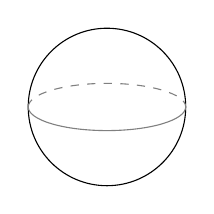
\begin{tikzpicture}
			% Outer circle
			\draw (0,0) circle (1);
			%3D
			\draw[gray] (-1,0) arc (180:360:1 and 0.3);
			\draw[gray,dashed] (-1,0) arc (180:0:1 and 0.3);
		\end{tikzpicture}\]
		y el homeomorfismo
		\[h_1(x,y,z)=(x,y).\]
	\end{ejem}
	\begin{ejem}[de un cambio de coordenadas]
		Tomemos un punto en $S^2$, por ejemplo $p=(\frac{1}{2},\frac{1}{2},\frac{1}{2})$, que está en $U_1$, y también en $U_2=\{(x,y,z)\in\R^3: x^2+y^2+z^2=1, y>0\}$ con $h_2=(x,z)$. Luego,
		\[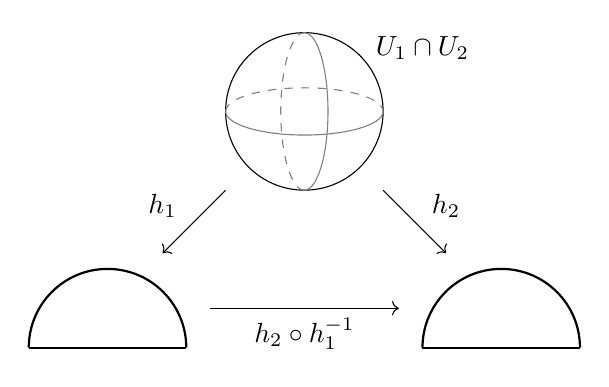
\begin{tikzpicture}
			% Sphere
			\draw (0,0) circle (1);
			\draw[gray] (-1,0) arc (180:360:1 and 0.3);
			\draw[gray,dashed] (-1,0) arc (180:0:1 and 0.3);
			\draw[gray,dashed] (0,-1) arc (270:90:0.3 and 1);
			\draw[gray] (0,1) arc (90:-90:0.3 and 1);
			\node at (1.5,0.8) {$U_1\cap U_2$};
			
			% Arrows and labels
			\draw[->] (-1,-1) -- (-1.8,-1.8);
			\node at (-1.8,-1.2) {$h_1$};
			\draw[->] (1,-1) -- (1.8,-1.8);
			\node at (1.8,-1.2) {$h_2$};
			\draw[->] (-1.2,-2.5) -- (1.2,-2.5) node[midway,below] {$h_2\circ h_1^{-1}$};
			
			% Left part
			\draw[thick] (-1.5,-3) arc (0:180:1);
			\draw[thick] (-1.5,-3) -- (-3.5,-3);
			
			% Right part
			\draw[thick] (1.5,-3) arc (180:0:1);
			\draw[thick] (1.5,-3) -- (3.5,-3);
		\end{tikzpicture}\]
		El cambio de coordenadas es $h_2\circ h_1^{-1}=(x,\sqrt{1-x^2-y^2})$, que es una función suave.
	\end{ejem}
	\begin{ejem}[El plano proyectivo real]
		En $\R^3\backslash\{(0,0,0)\}$ definamos la relación de equivalencia
		\[(x_1,y_1,z_1)\sim(x_2,y_2,z_2)\iff\exists\lambda\neq0\text{ tal que }(x_2,y_2,z_2)=\lambda(x_1,y_1,z_1)\]
		Como ejercicio se puede comprobar que en efecto se trata de una relación de equivalencia. El conjunto de clases de equivalencia se llama \textbf{plano proyectivo real} y de denota por $\R P^2$. A la clase de equivalencia de $(x_0,y_0,z_0)$ la denotamos $[x_0:y_0:z_0]$ y decimos que son las \textbf{coordenadas homogéneas} del punto.
		
		¿Cuáles serán las cartas?
		\begin{align*}
			\begin{aligned}
				U_0=\{[x:&y:z:]|x\neq0\}\\
				h_0:U_0&\to\R^2\\
				[x:y:z]&\mapsto\left(\frac{y}{x},\frac{z}{x}\right)
			\end{aligned}\qquad
			\begin{aligned}
				U_1=\{[x:&y:z:]|y\neq0\}\\
				h_1:U_1&\to\R^2\\
				[x:y:z]&\mapsto\left(\frac{x}{y},\frac{z}{y}\right)
			\end{aligned}\qquad
			\begin{aligned}
				U_2=\{[x:&y:z:]|z\neq0\}\\
				h_2:U_2&\to\R^2\\
				[x:y:z]&\mapsto\left(\frac{x}{z},\frac{y}{z}\right)
			\end{aligned}
		\end{align*}
		Observemos que $\R P^2=U_0\cup U_1\cup U_2$. Para encontrar los cambios de coordenadas, notemos que $h_1^{-1}=[u_1,1,v_1]$, de forma que $h_2\circ h_1^{-1}=h_2[u_1:1:v_1]=\left(\frac{u_1}{v_1},\frac{1}{v_1}\right)$, que es una función diferenciable.
		\[\begin{tikzcd}
			&U_1\cap U_2\arrow[swap]{ld}{h_1}\arrow{rd}{h_2}\\
			\R^2\arrow[swap]{rr}{h_2\circ h_1^{-1}}&&\R^2
		\end{tikzcd}\]
		Ahora definamos alguna función real-valuada en $\R P^2$ para ver si es suave. Tomemos el ejemplo de
		\begin{align*}
			f:\R P^2&\to \R\\
			f[x:y:z]=\arccos&\left(\frac{|z|}{\sqrt{x^2+y^2+z^2}}\right)
		\end{align*}
		que está bien definida ya que al multiplicar un vector en $\R^3\backslash\{(0,0,0\}$ por un escalar $\lambda$, éste se cancela. ¿Es suave? ¿Continua?
		
		Bueno, podemos darnos cuenta de que es continua cuando pensamos que el plano proyectivo es el hemisferio norte de la esfera identificando puntos antípodas en el ecuador. En este caso, casi todos los puntos del plano proyectivo tienen un único representante. Sólo los puntos en el ecuador podrían causar problema, pero la identificación por puntos antípodas en el ecuador nos permite construir vecindades de estos puntos pegando dos medias vecindades.
		\[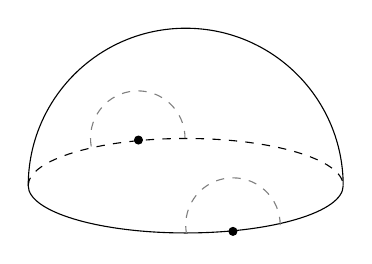
\begin{tikzpicture}[scale=2]
			% Outer circle
			\draw (-1,0) arc (180:0:1);
			%3D
			\draw (-1,0) arc (180:360:1 and 0.3);
			\draw[dashed] (-1,0) arc (180:0:1 and 0.3);
			
			\filldraw (-.3,.29) circle (0.025);
			\filldraw (.3,-.29) circle (0.025);
			
			\draw[gray,dashed] (-.6,.25) arc (190:0:0.3);
			\draw[gray,dashed] (.6,-.25) arc (0:190:0.3);
		\end{tikzpicture}\]
		Para saber si la función es suave, debemos llevar el problema a $\R^2$ usando las cartas coordenadas. Creemos que este ejemplo en particular no es suave…
		
		Tomemos mejor
		\[g[x:y:z]=\frac{ax+by+cz}{cx+dy+fz}\]
		Si $p\in U_2$,
		\begin{align*}
			g\circ h_2^{-1}(u_2,v_2)&=g[u_2:v_2:1]\\
			&=\frac{au_2+bv_2+e}{cu_2+dv_2+f}
		\end{align*}
		¿Cómo nos aseguramos de que no se puede hacer cero el denominador? Intentemos dar una función de la forma
		\begin{align*}
			G:\R P^2&\to\R P^1\approx\R\cup\{\infty\}\\
			[x:y:z]&\mapsto[ax+by+ez:cx+dy+fz]
		\end{align*}
		¡Hay elecciones de los coeficientes $a,\ldots,f$ que hacen que la función no sea suave!
	\end{ejem}
	\begin{ejer*}
		Consideremos para todo $r>0$ la aplicación $\varphi_r:\R\to\R$ dada por
		\begin{align*}
			\varphi_r(t)=
			\begin{cases}
				\begin{aligned}
					t\qquad&\text{si }t\leq0\\
					rt\qquad&\text{si }t\geq0
				\end{aligned}
			\end{cases}
		\end{align*}
		
		Muestre que los atlas $(\varphi_r)_{r>0}$ definen una familia no numerable de estructuras diferenciables sobre $\R$. ¿Las variedades diferenciables correspondientes son difeomorfas?
		\[\begin{tikzpicture}
			% Axes
			\draw[->] (-3,0) -- (3,0) node[right] {$t$};
			\draw[->] (0,-2) -- (0,3) node[above] {$\varphi_{1/2}(t)$};
			
			% Function plot
			\draw[blue, thick, domain=-2:0] plot (\x, \x);
			\draw[blue, thick, domain=0:3] plot (\x, 0.5*\x);
		\end{tikzpicture}\]
	\end{ejer*}
	\begin{proof}[Solución]
		Primero observemos que la función $\varphi_r$ es un homeomorfismo, ya que es continua y su inversa, $\varphi_{1/r}$, también. Al ser una única carta, los cambios de coordenadas son por vacuidad suaves, así que $\R$ con el atlas que consta de la carta $\varphi_r$ es una variedad diferenciable para toda $r$.
		
		Si $\R_r$ es la variedad con el atlas $\varphi_r$, ¿será que $\R_1$ es difeomorfa a $\R_{1/2}$? Intentemos dar un difeomorfismo:
		\begin{align*}
			f:\R_1&\to\R_{1/2}\\
			x&\mapsto\begin{cases}
				\begin{aligned}
					x\qquad&\text{si }x\leq0\\
					2x\qquad&\text{si }x\geq0
				\end{aligned}
			\end{cases}
		\end{align*}
		Claramente $f$ es biyectiva. ¿Será suave? Notemos que si consideramos esta función de $\R_1$ en $\R_1$ no lo es, pues tiene un pico en 0. Recordando nuestra definición de función suave entre variedades, consideremos el siguiente diagrama:
		\[\begin{tikzcd}
			&\R_1\arrow{r}{f}\arrow[swap]{d}{\varphi_1}&\R_{1/2}\arrow{d}{\varphi_{1/2}}\\
			&\R\arrow[dashed]{r}&\R
		\end{tikzcd}\]
		De hecho $\varphi_{1/2}\circ f\circ\varphi^{-1}_1=\varphi_{1/2}\circ f=id$, así que $f$ es suave. Y por un cálculo análogo, $f^{-1}$ también. Esta construcción se generaliza fácilmente para construir un difeomorfismo de $\R_1$ en $\R_r$, y con una simple composición, concluimos que todas estas variedades son difeomorfas entre sí.
	\end{proof}
	
	\section{Vectores tangentes}
	Recordemos que para el caso de superficies en $\R^3$ los vectores tangentes se pueden ver como el vector velocidad de una curva regular en la superficie. ¿Cómo podemos generalizar esta definición?
	\begin{defn}
		Sean $M$ una variedad diferenciable, $p\in M$ y $C^\infty(M,\R)$ el conjunto de funciones suaves $f:M\to\R$. Un \textbf{vector tangente} a $M$ en $p$ es un funcional $v:C^\infty(M,\R)\to\R$ con las propiedades de que
		\begin{itemize}
			\item \textbf{$\R$-lineal:} $v(\lambda f+\mu g)=\lambda v(f)+\mu v(g)$
			\item \textbf{Regla de Leibniz:} $v(f\cdot g)=v(f)g(p)+f(p)v(g)$
		\end{itemize}
	\end{defn}
	Este concepto generaliza la idea de \textit{derivada direccional}: cada vector tangente es un operador que actúa como una derivada direccional.
	
	\begin{obs}
		Sean $M$ una variedad diferenciable y $p\in M$. La colección de todos los vectores tangentes a $M$ en $p$ es un espacio vectorial con las siguientes operaciones:
		\begin{itemize}
			\item Elemento cero: $f\mapsto0$.
			\item Suma: $v+w:C^\infty(M,\R)\to\R$ tal que $f\mapsto v(f)+w(f)$
			\item Producto escalar. $\lambda v:C^\infty(M,\R)\to\R$ tal que $f\mapsto\lambda v(f)$
		\end{itemize}
	\end{obs}
	¿Cuál será una base de este espacio vectorial? Se nos antoja tomar los vectores canónicos en el dominio de la \textbf{parametrización} (la función inversa de la carta coordenada, cuyo dominio es $\R^n$).
	
	Consideremos una vecindad coordenada $U$ de $p\in M$ y la carta correspondiente
	\begin{align*}
		h:U\subset M&\to V\subset\R^n\\
		q&\mapsto (x^1(q),x^2(q),\ldots,x^n(q))
	\end{align*}
	Diremos que $x^i:U\subset M\to\R$ son las \textbf{funciones coordenadas}.
	
	Ahora tomemos una función suave en la variedad, $f:M\to\R$, y componemos con la parametrización para obtener
	\begin{align*}
		f\circ h^{-1}:V\subset\R^n&\to\R\\
		(u^1,u^2,\ldots,u^n)&\mapsto f\circ h^{-1}(u^1,u^2,\ldots,u^n)
	\end{align*}
	Esta función tiene una derivada direccional,
	\[\frac{\partial}{\partial x^i}(f):=\frac{\partial}{\partial u^i}\Big|_{h(p)}(f\circ h^{-1})\]
	Cuando variamos $f$, obtenemos un operador que es un candidato perfecto para ser un vector tangente. Resultará que éstos son una base del espacio tangente $T_pM$.
	\begin{lema}[No visto en clase, \cite{ONeill}]
		Sea $v\in T_pM$.
		\begin{enumerate}
			\item Si $f,g\in\Cinf(M,\R)$ son iguales en una vecindad de $p$, entonces $v(f)=v(g)$.
			\item Si $h\in\Cinf(M,\R)$ es constante, $v(f)=0$.
		\end{enumerate}
	\end{lema}
	\begin{lema}
		Sea $g:V\to\R$ suave, donde $V\subset\R^n$ es un conjunto abierto convexo que contiene al $0$. Entonces, existen funciones $g_i:V\subset\R^n\to\R$ suaves tales que
		\[g(u^1,\ldots,u^n)=g(0,\ldots,0)+\sum_{i=1}^ng_i(u^1,\ldots,u^n)u^i\]
		y además $g_i(0,\ldots,0)=\frac{\partial g}{\partial u^i}(0,\ldots,0)$
	\end{lema}
	\begin{proof}
		Proponemos
		\[g_i(u^1,\ldots,u^n)=\int_0^1\frac{\partial g}{\partial u^i}(tu^1,\ldots,tu^n)dt.\]
		Hagamos un poco más explícitas las cuentas hechas en clase. Cuando fijamos un punto $(u^1,\ldots,u^n):=q\in\R^n$, podemos ver la función $g(tq)$ como una función de $\R$ en $\R$. ¿Cuál es su derivada? Debemos usar la regla de la cadena pensando en la composición de "multiplicar por $t$" seguida de $g$:
		\[d_t g(tq)=d_{tq}g\cdot d_t(tq)=\nabla_{tq}g\cdot q\]
		Donde $\cdot$ es el producto de matrices (en este caso es el producto punto), y $\nabla g$ es el vector de derivadas parciales. Luego aplicamos el teorema fundamental del cálculo para obtener:
		\begin{align*}
			g(u^1,\ldots,u^n)-g_i(0,\ldots,0)&=\int_0^1\frac{dg}{dt}(tu^1,\ldots,tu^n)dt\\
			&=\sum_{i=1}^n\int_0^1\frac{\partial g}{\partial u^i}(tu^1,\ldots,tu^n)u^idt\\
			&=\sum_{i=1}^nu^i\int_0^1\frac{\partial g}{\partial u^i}(tu^1,\ldots,tu^n)dt
		\end{align*}
	\end{proof}
	Lo anterior se puede expresar así:
	\begin{equation}\label{ec1}
		g=g(0)+\sum g_iu^i
	\end{equation}
	\begin{teo}[\textbf{12}, \cite{ONeill}]\label{teo:base}
		Si $h(q)=(x^1(q),\ldots,x^n(q))$ es una carta coordenada de $M$ en $p$, entonces los vectores $\frac{\partial}{\partial x^1}, \ldots, \frac{\partial}{\partial x^n}
		$ son una base del espacio tangente. Más aún,
		\[v = \sum_{i=1}^n v(x^i) \frac{\partial}{\partial x^i} \qquad \text{para toda } v \in T_pM\]
	\end{teo}
	\begin{proof}
		Tomemos $f\in\Cinf(M,\R)$ y definimos $g:=f\circ h^{-1}$ para usar el lema. Suponiendo que $h(p)=0$, sustituyendo en \ref{ec1}, obtenemos que 
		\[f=f(p)+\sum f_ix^i\]
		donde $f_i=\int_0^1\frac{\partial f}{\partial x^i}(tq)dt$. Derivando esta expresión respecto a $x^i$ simplemente obtenemos
		\begin{equation}\label{ec2}
			\frac{\partial f}{\partial x^i}=f_i
		\end{equation}
		Ahora sea $v\in T_pM$ cualquier vector tangente. Al aplicar $f$ obtenemos:
		\begin{align*}
			v(f) &= v\left(f(p)+\sum_{i=1}^nf_ix^i\right) \\
			&= v\left(f(p)\right)+v\left(\sum f_i x^i\right) \\
			&=0+ \sum v\left(f_i x^i\right)\qquad\qquad\text{ya que }f(p)\text{ es constante} \\
			&=\sum v(f_i)x^i(p)+f_i(p)v(x^i)\qquad\text{Leibniz}\\
			&=0+\sum \frac{\partial f_i}{\partial x^i}x^i\qquad\qquad\text{ya que }h(p)=0\text{ y por }\ref{ec2}
		\end{align*}
		Ahora veamos que los vectores son linealmente independientes. Supongamos que
		\[w:=\sum\alpha_i\frac{\partial}{\partial{x^i}}\Bigg|_{p}=0\in T_pM\]
		Evaluando en $x^j\in\Cinf$,
		\[0=w(x^j)=\sum\alpha_i\frac{\partial x^j}{\partial{x^i}}\Bigg|_{p}=\alpha_j\]
	\end{proof}
	\section{Diferencial de una aplicación}
	Dadas dos variedades $M$ y $N$, la \textbf{diferencial} de una función $\phi:M\to N$ en $p\in M$ es de la forma
	\begin{align*}
		d\phi_p:T_pM&\to T_pN\\
		v&\mapsto d\phi_p(v)
	\end{align*}
	La asociación es bastante natural: $d\phi_p(v)$ manda una función $f\in\Cinf(N,\R)$ en $v(f\circ\phi)$.
	\[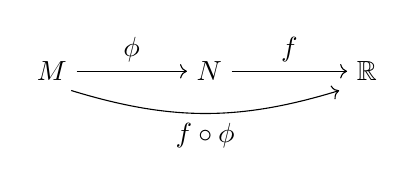
\begin{tikzpicture}
		\node (A) at (0,0) {$M$};
		\node (B) at (2,0) {$N$};
		\node (C) at (4,0) {$\R$};
		\draw[->] (A) -- node[above] {$\phi$}(B);
		\draw[->] (B) -- node[above] {$f$} (C);
		\draw[->, bend right=17] ([xshift=7pt]A.south) to node[below] {$f\circ\phi$} ([xshift=-10pt]C.south);
	\end{tikzpicture}\]
	\begin{obs}
		La diferencial es una transformación lineal.
	\end{obs}
	\begin{lema}[\textbf{14}, \cite{ONeill}]\label{lema:dif-coord}
		Sean $\phi:M\to N$ una transformación suave, $p\in M$ y $q=\phi(p)\in N$ con sistemas de coordenadas $h:U\subset M\to\R^m$ y $k:V\subset N\to\R^n$ tales que $h(p)=0$, y $k(q)=0$. Entonces,
		\[d\phi_p\left(\frac{\partial}{\partial x^j}\Big|_p\right)=\sum_{i=1}^n\frac{\partial(y^i\circ\phi)}{\partial x^j}(p)\frac{\partial}{\partial y^i}\Big|_{\phi p}\]
		Con funciones coordenadas  $h=(x^1,\ldots,x^m)$ y $k=(y^1,\ldots,y^n)$.
	\end{lema}
	\begin{proof}
		Definamos $v=\frac{\partial}{\partial x^j}\in T_pM$ y tomemos una función $g\in\Cinf(N,\R)$. Para encontrar $d\phi_p(v):=w$, usamos el \hyperref[teo:base]{teorema} anterior para expresar
		\begin{align*}
			w=\sum_{i=1}^nw(y^i)\frac{\partial}{\partial y^i}
		\end{align*}
		Y luego calculamos
		\[w(y^i)=v(y^i\circ\phi)=\frac{\partial}{\partial x^j}\Big|_py^i\circ\phi\]
	\end{proof}
	\begin{obs}
		Con toda formalidad, la expresión anterior es de la forma
		\[\frac{\partial}{\partial x^j}\Big|_py^i\circ\phi\\
		=\frac{\partial}{\partial u^j}\Big|_0y^i\circ\phi\circ h^{-1}	\]
	\end{obs}
	\begin{obs}\label{obs:dif-mat}
		Recordando que la diferencial es una transformación lineal entre los espacios tangentes, la matriz que la representa respecto a las bases $\left\{ \frac{\partial}{\partial x^1},\ldots,\frac{\partial}{\partial x^m}\right\}$ y $\left\{\frac{\partial}{\partial y^1},\ldots,\frac{\partial}{\partial y^n}\right\}$ es igual a la matriz que representa la derivada de la transformación en coordenadas respecto a las bases canónicas de los espacios euclideanos.
		
		Con todo detalle, sea $A=(a_{ij})$ la matrix de $n\times m$ coorespondiente a $d\phi_p$. Es decir,
		\[d\phi_p\left(\frac{\partial}{\partial x^j}\Big|_p\right)=\sum_{i=1}^na_{ij}\frac{\partial}{\partial y^i}\Big|_q\]
		De acuerdo al \hyperref[lema:dif-coord]{lema} anterior, $a_{ij}=\frac{\partial y^i\circ\phi\circ h^{-1}}{\partial x^j}$.
		
		La derivada de la transforamción en coordenadas es $d(k\circ\phi\circ h^{-1})_0$. Se trata de una transformación lineal $B:\R^m\to\R^n$. Recordando que las funciones coordenadas en el contradominio son $k=(y^1,\ldots,y^n)$, la representación matricial de $B$ es $\left(\frac{\partial y^i\circ\phi\circ h^{-1}}{\partial x_j}\right)_{ij}$.
	\end{obs}
	\section{Subvariedades}
	\begin{defn}
		Una \textbf{subvariedad} de $S$ de una variedad $M$ es una variedad tal que:
		\begin{enumerate}
			\item[\textit{i)}] Tiene la topología de subespacio de $M$.
			\item[\textit{ii)}] La inclusión $j:S\hookrightarrow M$ es suave y en cada punto $p\in S$ la diferencial de $j$ en $p$ $dj_p:T_pS\to T_pS$ es inyectiva.
		\end{enumerate}
	\end{defn}
	\begin{ejem}[Lemniscata]
		Pensamos una función $\alpha:\R\to L$, donde $L$ es la Lemniscata. Cuando le damos la topología inducida por $\alpha$, resulta que esta curva es una variedad. Sin embargo, no es una subvariedad de $\R^2$ con la topología usual de acuerdo a la definición que acabamos de dar.
		\[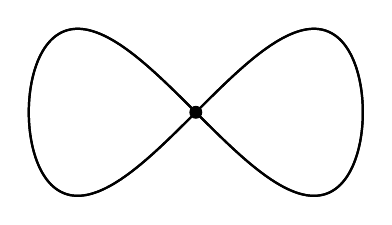
\begin{tikzpicture}[scale=1.5]
			
			\draw[thick, domain=0:360, samples=500] plot ({sqrt(2) * cos(\x)} , {sqrt(2) * cos(\x) * sin(\x)});
			\draw[thick, domain=0:360, samples=500] plot ({-sqrt(2) * cos(\x)} , {-sqrt(2) * cos(\x) * sin(\x)});
			
			\draw[fill=black] (0,0) circle (0.05);
		\end{tikzpicture}\]
	\end{ejem}
	\begin{ejem}[La gráfica del valor abosluto]
		Consideremos $S=\{(x,y)\in\R^2:y=|x|\}$, que es una subvariedad topológica de $\R^2$ con la topología usual.
		\[\begin{tikzpicture}
			% Axes
			\draw[->] (-3,0) -- (3,0) node[right] {$x$};
			\draw[->] (0,-.5) -- (0,3) node[above] {$|x|$};
			
			% Absolute value function plot
			\draw[blue, thick, domain=-3:3, samples=100] plot (\x, {abs(\x)});
		\end{tikzpicture}\]
		\begin{af}
			No existe ninguna estructura suave para $S$ tal que $S$ sea subvariedad de $\R^2$.
		\end{af}
		Supongamos que tenemos una carta coordenada $h$ en a algún atlas de $S$ y un vector $v\in T_pS$ cuya imagen bajo la diferencial $di_p$ es cero.
		\[\begin{tikzcd}
			S\arrow[hook]{r}{j}\arrow[swap]{d}{h}&\R^2\arrow{d}{id}\\
			\R\arrow[dashed]{r}&\R^2
		\end{tikzcd}\]		
		Notemos que la parametrización local es de la forma $h^{-1}(t)=(x,y)$ con $y=|x|$, o bien $y^2(t)=x^2(t)$. Derivando, $2y(t)y'(t)=2x(t)x'(t)$. Tenemos dos casos:
		\begin{itemize}
			\item Si $x(t)>0$, entonces $y(t)=x(t)$ y $y'(t)=x'(t)$. Tomando límite hacia el cero ya que las funciones son suaves, $y'(0)=x'(0)$.
			\item Si $x(t)<0$ entonces $y(t)=-x(t)$ y $y'(t)=-x'(t)$. Tomando límite, $y'(0)=x'(0)$.
		\end{itemize}
		\textit{*Falta concluir que ambas derivadas son cero*}
	\end{ejem} 
	\begin{obs}
		En \cite{Lee}, tenemos otra demostración de este hecho en el \textbf{Ejemplo 5.45}. Esencialmente, Lee usa la siguiente proposición:
		\begin{prop}
			Sean $M$ una variedad, $S\subset M$ una subvariedad, $p\in S$ y $v\in T_pM$. Entonces $v$ es un vector en $T_pS$ si y sólo si existe una curva suave $\gamma:J\to M$ cuya imagen está contenida en $S$, es suave como mapeo en $S$, y es tal que $0\in J$, $\gamma(0)=p$ y $\gamma'(0)=v$.
		\end{prop}
		Suponiendo que $S$ es una subvariedad, tendríamos una curva suave $\gamma:(-\varepsilon,\varepsilon)\to\R$ que en $0$ pasa por $(0,0)$ y su derivada no es cero, ya que el espacio tangente debe tener al menos un elemento no trivial. Si $\gamma(t)=(x(t),y(t))$, la función $y$ alcanza un mínimo en $t=0$, así que $y'(0)=0$. Y, como en la prueba que hicimos en clase, sabemos que $y^2(t)=x^2(t)$. Derivando dos veces, $y'(t)^2+y(t)y''(t)=x'(t)^2+x''(t)$. Evaluando en $t=0$, concluimos que $y'(t)=x'(t)=0$, pero esto es justo lo que no queríamos.
	\end{obs}
	
	
	
	\clearpage
	\subsection{Ejercicios 14-18 de agosto}
	Sea $M$ una variedad diferenciable de dimensión $m$ y $N$ una variedad diferenciable de dimensión $n$. Sea $p\in M$, $U$ una vecindad coordenada de $p$ con una carta $h:U\subset M\to\R^m$. Sea $q\in N$, $V$ una vecindad coordenada de $q$ con una carta $k:V\subset N\to\R^n$. A $M\times N$ le damos estructura de variedad, cuyas vecindades coordenadas son de la forma $U_\alpha\times V_\beta$, y cuyas cartas son de la forma 
	\begin{align*}
		h\times k:U_\alpha\times V_\beta&\to\R^m\times\R^n\\
		(p,q)&\mapsto \left(h(p),k(q)\right)
	\end{align*}
	\begin{enumerate}
		\item Las proyecciones 
		\begin{align*}
			\begin{aligned}
				\pi:M\times N&\to M\\
				(p,q)&\mapsto p
			\end{aligned}
			\qquad\text{ y }\qquad
			\begin{aligned}
				\sigma:M\times N&\to N\\
				(p,q)&\mapsto q
			\end{aligned}
		\end{align*}
		son suaves.
		
		\item Una transformación $\phi:P\to M\times N$ es suave si y sólo si $\pi\circ\phi$ y $\sigma\circ\phi$ son suaves.
		\item Para cada $(p,q)\in M\times N$ los subconjuntos
		\begin{align*}
			M\times q=\{(x,q)\in M\times N:x\in M\}\\
			p\times N=\{(p,y)\in M\times N:y\in N\}
		\end{align*}
		son subvariedades de $M\times N$.
		\item Para cada $(p,q)$,
		\begin{align*}
			\pi|_{M\times q}\text{ es un difeomorfismo }M\times q\to M\\
			\sigma|_{p\times N}\text{ es un difeomorfismo }p\times N\to N
		\end{align*}
	\end{enumerate}
	\begin{proof}[Solución]\leavevmode
		\begin{enumerate}
			\item Escogiendo un punto en $M\times N$ y una carta corrdenada $h\times k$, construimos el siguiente diagrama:
			\[\begin{tikzcd}
				M\times N\arrow{r}{\pi}\arrow[swap]{d}{h\times k}&M\arrow{d}{h}\\
				\R^m\times\R^n\arrow[dashed]{r}&\R^m
			\end{tikzcd}\]
			La flecha punteada manda $(x,y)\mapsto x$, que es suave.
			\item Para un punto en $P$ con carta coordenada $\ell$ tal que $h\times k$ es una carta de su imagen bajo $\phi$, tenemos:
			\[\begin{tikzcd}
				P\arrow{r}{\phi}\arrow[swap]{d}{\ell}&M\times N\arrow{d}{h\times k}\\
				\R^p\arrow[dashed]{r}&\R^m\times\R^n
			\end{tikzcd}\]
			Sabemos que $P$ es suave si y sólo si $(h\times k)\circ\phi\circ\ell^{-1}$ es suave.  Notemos que para $z\in\R^p$, $\left(h\times k)\left(\phi\left(\ell^{-1}(z)\right)\right)=\left(h\left(\phi\left(\ell^{-1}(z)\right)\right),k(\phi\left(\ell^{-1}(z)\right)\right)\right)$, de manera que la flecha punteada es suave cuando las dos funciones coordenadas son suaves, y de hecho, ¡éstas son las cartas coordenadas cuando componemos con las proyecciones!
			\item Primero debemos dar una estructura diferenciable para $M\times q$. Dado $(x,q)\in M\times q$ tomemos cualquier carta  $h:U_\alpha\to\R^m$ de $M$ que contenga a $x$ y definamos ${h\times q:U_\alpha\times\{q\}\to\R^m}$ simplemente por $(h\times q)(y,q)=h(y)$.
			
			Ahora veamos si la inclusión es suave mediante el siguiente diagrama:
			\[\begin{tikzcd}
				M\times q\arrow[hook]{r}{j}\arrow[swap]{d}{h\times q}&M\times N\arrow{d}{h\times k}\\
				\R^m\arrow[dashed]{r}&\R^m\times\R^n
			\end{tikzcd}\]
			Notemos que hemos usado la carta $h$ en dos lugares distintos. La flecha punteada es la inclusión $\R^m\hookrightarrow\R^m\times\R^n$, que es suave. Para ver que su diferencial es inyectiva, usamos la \hyperref[obs:dif-mat]{observación} de que la matriz que representa a la diferencial es la misma que la matriz de la derivada de la transformación en coordenadas, que es $\begin{pmatrix}
				id_{m}\\0_{n}
			\end{pmatrix}$, y en particular es inyectiva.
			
			\textbf{Otro camino}: supongamos que $v\in T_{M\times q}$ es tal que $dj_pv=0$. Para ver que $v=0$, tomemos $f\in\Cinf(M\times q,\R)$. Consideremos la función $\tilde{f}\in\Cinf(M\times N,\R)$ dada por $\tilde{f}(x,y)=f(x,q)$, que es suave ya que la derivada de $\tilde{f}\circ(h\times k)^{-1}$ es el vector $(df_p,0,\ldots,0)$. Luego, $v(f)=v(\tilde{f}\circ j)=dj_pv(\tilde{f})=0$.
			\item La restricción de una función suave a una subvariedad es suave. Para dar una demostración explícita, tomamos cartas coordenadas alrededor de algún punto para construir el siguiente diagrama:
			\[\begin{tikzcd}
				M\times q\arrow{r}{\pi|_{M\times q}}\arrow[swap]{d}{h\times q}&M\arrow{d}{h}\\
				\R^m\arrow[dashed]{r}&\R^m
			\end{tikzcd}\]
			La flecha punteada es la identidad. El caso de la función inversa es análogo.
		\end{enumerate}
	\end{proof}
	\begin{ejem}[de una variedad producto]
		Consideremos $S^1=\{(x,y)\in\R^2|x^2+y^2=1\}$ con el atlas
		\begin{align*}
			\begin{aligned}
				&h_N(x,y)=x\\
				&U_N=\{(x,y)\in S^1|y>0\}\\\\
				&h_O(x,y)=y\\
				&U_E=\{(x,y)\in S^1|x<0\}
			\end{aligned}
			\qquad
			\begin{aligned}
				&h_S(x,y)=y\\
				&U_S=\{(x,y)\in S^1|y<0\}\\\\
				&h_E(x,y)=y\\
				&U_E=\{(x,y)\in S^1|x>0\}
			\end{aligned}
		\end{align*}
		Que son las proyecciones al eje $x$ o $y$.
		\[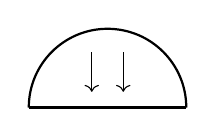
\begin{tikzpicture}
			\draw[thick] (1,0) arc (0:180:1);
			\draw[thick] (-1,0) -- (1,0);
			\draw[->] (-.2,0.7)--(-.2,0.2);
			\draw[->] (.2,0.7)--(.2,0.2);
		\end{tikzpicture}\]
		Ahora sea $S^1\times S^1$ con las cartas producto, que son de la forma
		\begin{align*}
			h_N\times h_N:U_N\times U_N\subset S^1\times S^1&\to\R\times\R\approx\R^2\\
			\left((x_1,x_2),(y_1,y_2)\right)&\mapsto\left(h_N(x_1,x_2),h_N(y_1,y_2)\right)=(x_1,y_1)
		\end{align*}
		Podemos definir un atlas análogo en esferas de cualquier dimensión proyectando cada hemisferio al plano que lo determina.
		\[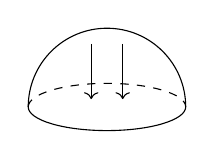
\begin{tikzpicture}[scale=1]
			\draw (-1,0) arc (180:0:1);
			\draw (-1,0) arc (180:360:1 and 0.3);
			\draw[dashed] (-1,0) arc (180:0:1 and 0.3);
			\draw[->] (-.2,0.8)--(-.2,0.1);
			\draw[->] (.2,0.8)--(.2,0.1);
		\end{tikzpicture}\]
		Para el caso de $S^2$, tenemos la figura de \cite{DoCarmo}:
		\begin{center}
			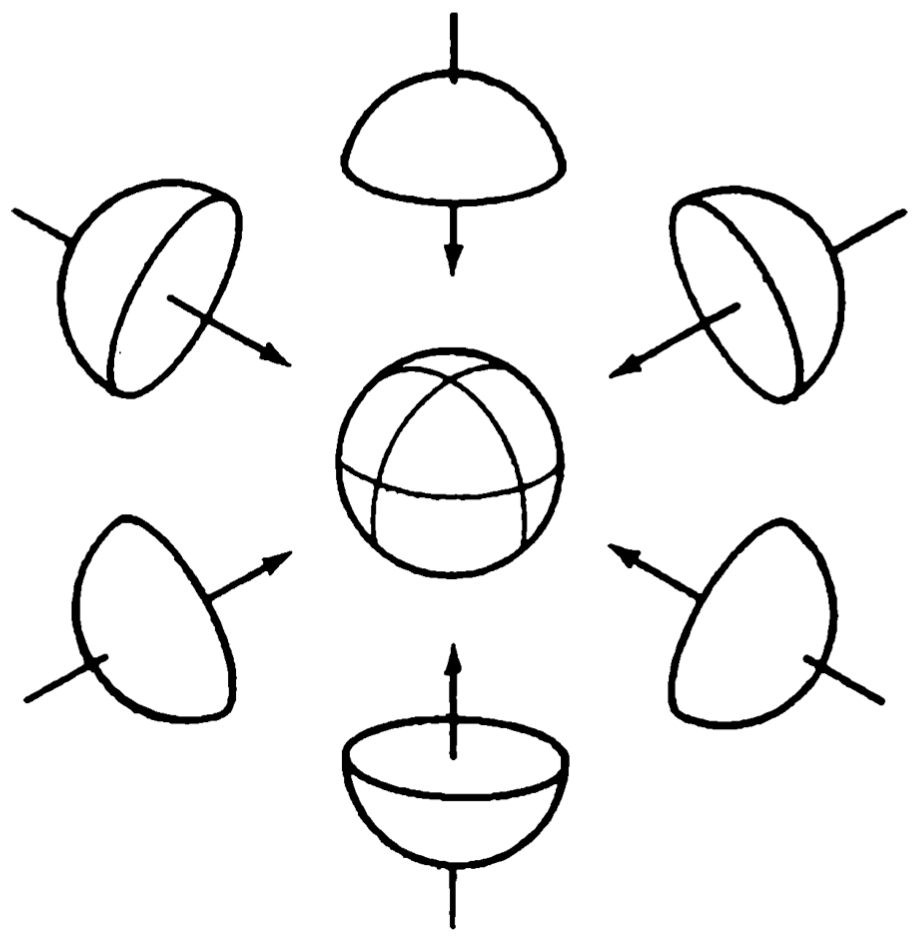
\includegraphics[width=0.5\linewidth]{fig1.png}
		\end{center}
		Con estas estructuras diferenciables podemos construir la variedad $S^p\times S^q$. (También podemos usar las proyecciones estereográficas desde el polo norte y el polo sur para cubrir a la esfera con sólo dos cartas).
	\end{ejem}
	\section{Inmersiones, sumersiones y encajes}
	\begin{defn}
		Una función suave entre variedades $f:M\to N$ es una \textbf{inmersión} en $p\in M$ si su diferencial es inyectiva en $p$, y es una \textbf{sumersión} si su diferencial es suprayectiva dn $p$. Si esta condición se cumple en toda $M$, decimos que la función es una inmersión o una sumersión.
	\end{defn}
	\begin{obs}
		En la definición de subvariedad pedimos que la inclusión sea una inmersión.
	\end{obs}
	\begin{obs}
		¿Qué quieren decir estas condiciones? Observemos que por el teorema de la dimensión, si la diferencial $df_p:T_pM\to T_{f(p)}N$ es inyectiva, se sigue que $\dim M\leq\dim N$. Análogamente, si la diferencial es suprayectiva, $\dim N\leq\dim M$.
	\end{obs}
	\begin{ejem}
		Los ejemplos canónicos de inmersiones y sumersiones son la inclusión y la proyección de espacios euclidianos:
		\begin{align*}
			i:\R^m&\hookrightarrow\R^n\\
			(x^1,\ldots,x^m)&\mapsto(x^1,\ldots,x^m,0,\ldots,0)
			\\\\
			\pi:\R^n&\to\R^m\\
			(x^1,\ldots,x^n)&\mapsto(x^1,\ldots,x^m)
		\end{align*}
		para $m\geq n$.
	\end{ejem}
	\begin{defn}
		Un \textbf{encaje} es una inmersión que también es un homeomorfismo en su imagen.
	\end{defn}
	\begin{ejem}[Curva densa en el toro, \cite{Lee} \textbf{, 4.20}]
		Consideremos el toro como la variedad producto $T^2=S^1\times S^1\subset\C^2$. Tomemos un número irracional $\alpha$ y la siguiente curva:
		\begin{align*}
			\gamma:\R&\to T^2\\
			t&\mapsto(e^{2\pi it},e^{2\pi i\alpha t})
		\end{align*}
		Primero notemos que $\gamma$ es una inmersión, ya que es suave y $\gamma'(t)$ nunca se anula (como transformación lineal, $\gamma'(t):\R\to\R^4$ sólo puede enviar un número real $\neq0$ al cero si todas sus entradas son cero).
		
		De hecho es una función inyectiva, ya que
		\begin{align*}
			\gamma(t_1)&=\gamma(t_2)\\
			\iff (e^{2 \pi it_1},e^{2\pi i\alpha t_1})&=(e^{2\pi it_2},e^{2\pi i\alpha t_2})\\
			\iff e^{2\pi it_1}=e^{2\pi it_2}\quad&\text{y}\quad e^{2\pi i\alpha t_1}=e^{2\pi\alpha it_2}\\
			\iff t_1=t_2+m\quad&\text{y}\quad\alpha t_1=\alpha t_2+n\quad\text{para }m,n\in\Z\\
			\iff t_1-t_2=m\quad&\text{y}\quad \alpha t_1-\alpha t_2=n\\
			\implies\alpha m&=n
		\end{align*}
		que sólo es posible si $m=n=0$.
		
		Ahora probaremos que $\gamma$ no es un encaje, pues no es un homeomorfismo en su imagen. Mostraremos que hay puntos en la curva $\gamma$ tan cercanos como queramos al $(1,1)\in \gamma$. Pensemos en qué pasa cada vez que avanzamos sobre $\gamma$ por un número entero: la primera coordenada vuelve a ser 1, pero la segunda cambia. La idea es encontrar un número entero $n$ tal que al desplazarse por $n$ la segunda coordenada sea tan cercana como queramos al 1. Es decir, queremos encontrar una cota para $|e^{2\pi i\alpha n}-1|$.
		
		Notemos que $|e^{2\pi it_1}-e^{2\pi it_2}|\leq|t_1-t_2|$.
		\[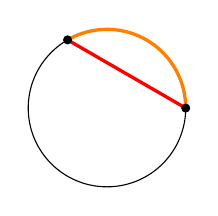
\begin{tikzpicture}
			\draw (0,0) circle (1);
			\draw[very thick,orange] (1,0) arc (0:120:1);
			\draw[very thick, red] (1,0)--(-.5,.866);
			\draw[fill=black] (-.5,.866) circle (0.05);
			\draw[fill=black] (1,0) circle (0.05);
		\end{tikzpicture}\]
		Ahora tomamos dos números enteros $n$ y $m$. Tenemos:
		\[|e^{2\pi i\alpha n}-1|=|e^{2\pi i\alpha n}-e^{2\pi im}|\leq|2\pi i\alpha n-2\pi im|=2\pi|\alpha n-m|\]
		
		Necesitaremos el siguiente lema:
		\begin{lema}[Teorema de aproximación de Dirichlet]
			Sea $\alpha$ un número real. Hay un múltiplo entero de $\alpha$ que es muy cercano a algún número entero. Es decir, para cualquier entero positivo $N$, existen enteros $n,m$ con $1\leq n\leq N$ tales que ${|n\alpha-m|<1/N}$.
		\end{lema}
		\begin{proof}
			Para los múltiplos enteros de $\alpha$, consideremos su distancia al entero menor o igual más cercano, $|k\alpha-\lfloor k\alpha\rfloor|$, que son números en el intervalo $[0,1)$. Dividamos el intervalo en $N$ partes de tamaño $1/N$. Consideremos $k=0,1,\ldots,N$. Se trata de $N+1$ puntos repartidos en $N$ intervalos, de manera que existen dos en uno sólo, digamos $k_1$ y $k_2$. Escojamos $n=k_2-k_1$ y $m=\lfloor k_2\rfloor-\lfloor k_1\rfloor$. Luego,
			\begin{align*}
				1/N&>\Big||k_1\alpha-\lfloor k_1\alpha\rfloor|-|k_2\alpha-\lfloor k_2\alpha\rfloor|\Big|\\
				&\geq|(k_1\alpha-\lfloor k_1\alpha\rfloor)-(k_2\alpha-\lfloor k_2\alpha\rfloor)|\\
				&\geq|\alpha(k_1-k_2)-(\lfloor k_2\alpha\rfloor-\lfloor k_1\alpha\rfloor)|
			\end{align*}
		\end{proof}
		Por lo tanto, existe $n$ entero tal que $|e^{2\pi i\alpha n}-1|<2\pi\varepsilon$ para cualquier $\varepsilon>0.$ De hecho,
		\[|\gamma(n)-\gamma(0)|=|(e^{2\pi in},e^{2\pi i\alpha n})-(1,1)|=|(1,e^{2\pi i\alpha} n)|=|e^{2\pi i\alpha n}-1|<2\pi\varepsilon\]
		De forma que $(1,1)$ es un punto de acumulación de $\gamma(\Z)$, y los homeomorfismos (hay que considerar $\gamma^{-1}$) mandan puntos de acumulación en puntos de acumulación, pero el 0 no es punto de acumulación de $\Z$ en $\R$.
		\begin{figure}[H]
			\centering
			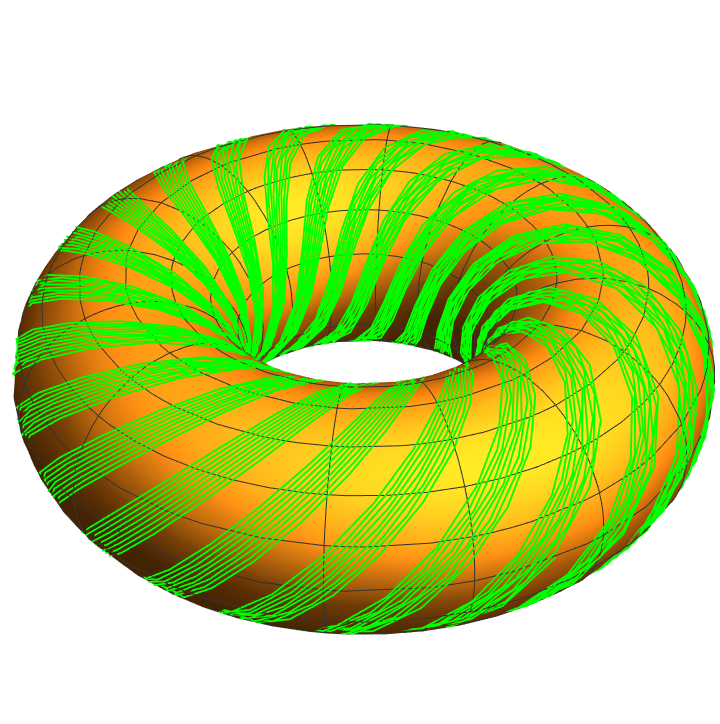
\includegraphics[width=0.5\textwidth]{fig9}
			\caption*{La curva $\gamma$ para $\alpha=\pi$ con $t\in[0,400]$}
		\end{figure}
	\end{ejem}
	Ahora mostraremos una propiedad sobre las sumersiones.
	
	\begin{teo}[del conjunto de nivel regular, \cite{Loring}\textbf{, 9.9}]
		Sea $f:M\to N$ una función suave entre las variedades $M$ y $N$. Si hay un punto $c\in N$ tal que $f$ es una sumersión en todos los puntos de $f^{-1}(c)$, entonces $f^{-1}(c)$ es una subvariedad de $M$ de dimensión $m-n$.
	\end{teo}
	\begin{proof}
		Para alguna carta $k$ alrededor de $c\in N$, nombremos las coordenadas de $f$ mediante $k\circ f=(f^1,\ldots,f^n)\in\R^n$.
		
		La idea es demostrar que dada una carta $h=(x^1,\ldots,x^m)$ en $M$, podemos reemplazar las primeras $n$ funciones coordenadas con las coordenadas de $f$. Es decir, que la función
		\begin{align*}
			\tilde{h}:M&\to\R^n\\
			p&\mapsto(f^1,\ldots,f^n,x^{n+1},\ldots,x^{m})
		\end{align*}
		también es una carta.
		\[	\begin{tikzcd}
			M\arrow{r}{f}\arrow[swap]{d}{h,\tilde{h}}&N\arrow{d}{k}\\
			\R^m&\R^n
		\end{tikzcd}\]
		
		
		Basta ver que $\tilde{h}$ tiene inversa. Usaremos el teorema de la función inversa (\cite{Loring}\textbf{, 6.25}) para variedades: a reserva de los detalles, una función entre variedades es localmente invertible si y sólo si el determinante su diferencial no es cero.
		
		Para aplicar este teorema a $\tilde{h}$, notemos que su diferencial es la matriz 
		\[d\tilde{h}_p=\begin{pmatrix}
			D&X\\
			0&\Id
		\end{pmatrix}\]
		Donde $D$ es la submatriz de $df_p$ con las primeras $n$ columnas y $n$ renglones, y $X$ es el resto de esta matriz. (Recordemos que como $f$ es sumersión $n\geq m$, así que $df_p$ es una matrix de $m\times n$).
		
		Como $f$ es una sumersión en $f^{-1}(c)$, su diferencial $df_p=\left(\frac{\partial f_i}{\partial x^j}\right)$ tiene rango $n$. Renombrando las coordenadas para que las primeras $n$ funciones coordenadas de $df_p$ sean linealmente independientes, tenemos que $\det D\neq0$. Luego, $\det d\tilde{h}_p=\det D\det\Id\neq0$.
		
		Suponiendo que $k(c)=(0,\ldots,0)$, los puntos en $f^{-1}(c)$ tienen coordenadas en $\tilde{h}$ de la forma
		\[(0,\ldots,0,x^{n+1},\ldots,x^{m})\]
		lo que le da una estructura de $(m-n)$-variedad.
	\end{proof}
	\begin{defn}
		El \textbf{rango} de una función suave entre variedades es el rango de su diferencial.
	\end{defn}
	\begin{teo}[del rango constante, \cite{Loring}\textbf{, 11.1}]
		Sea $f:M\to N$ una función suave entre las variedades $M$ y $N$. Si el rango de $f$ es constante $k$ en una vecindad de algún punto $p\in M$, entonces existen cartas coordenadas $h:U\subset M\to\R^m$ y $k:V\subset N\to\R^n$ tales que
		\[(k\circ f\circ h^{-1}(r^1,\ldots,r^m)=(r^1,\ldots,r^m,0,\ldots,0)\]
		para cualquier $(r^1,\ldots,r^m)\in h(U)$.
	\end{teo}
	En otras palabras, $f$ se ve localmente como una inclusión (si es una inmersión) o como una proyección (si es una sumersión).
	
	\section{Campos vectoriales}\label{sec:campos-vectoriales}
	\begin{defn}[\cite{ONeill}]
		Un \textbf{campo vectorial} es una correspondencia que a cada $p\in M$ le asocia un vector tangente $v\in T_pM$, y \textit{varía suavemente} sobre la variedad.
	\end{defn}
	Debemos especificar qué quiere decir que el campo vectorial "varíe suavemente". Consideremos un vector tangente $v_p$ a una variedad $M$ anclado en el punto $p\in M$. Hemos visto que que deben existir coeficientes $a_i(p)$ tales que
	\[v_p=a_1(p)\frac{\partial}{\partial x^1}\Big|_p+\ldots+a_n(p)\frac{\partial}{\partial x^n}\Big|_p\]
	Suponiendo que $v_p$ es un elemento de un campo vectorial, podemos variar el punto en el que está anclado el vector para obtener otros vectores $v_q$ que se expresan análogamente como
	\[v_q=a_1(q)\frac{\partial}{\partial x^1}\Big|_q+\ldots+a_n(q)\frac{\partial}{\partial x^n}\Big|_q\]
	Decimos que un campo vectorial es \textbf{suave} si las funciones $a_1,\ldots,a_n:U\subset M\to\R$ son suaves.
	\begin{obs}
		Denotaremos al conjunto de campos vectoriales en una variedad por $\mathfrak{X}(M)$.
	\end{obs}
	Para definir un campo vectorial como una función entre dos conjuntos, primero debemos construir el haz tangente (ver \cite{Lee} \textbf{Cap 3.4}).
	\begin{defn}
		Dada una variedad $M$, el \textbf{haz tangente} es la unión disjunta de los espacios tangentes en cada punto, es decir,
		\[TM=\bigsqcup_{p\in M}T_pM\]
		La \textbf{proyección natural} es una función $\pi:TM\to M$ que envía cada vector en el punto al que está anclado.
		Un \textbf{campo vectorial} (\cite{Lee} \textbf{Cap. 8}) es una sección de la proyección natural, es decir, una función continua
		\begin{align*}
			V:M&\to TM\\
			p&\mapsto V_p
		\end{align*}
		tal que $\pi\circ V=\Id_M$.
		\[\begin{tikzcd}
			&TM\arrow{d}{\pi}\\
			M\arrow[dashed]{ur}{V}\arrow[swap]{r}{\Id}&M
		\end{tikzcd}\]
	\end{defn}
	\begin{prop}[\cite{Lee}\textbf{, 3.18}]
		Sea $M$ es una variedad de dimensión $n$. El haz tangente tiene una topología natural y una estructura suave que lo hacen una variedad diferenciable de dimensión $2n$ respecto a la cual $\pi:TM\to M$ es suave.
	\end{prop}
	\begin{proof}
		Comenzamos con una carta $h:U\subset M\to \R^n$ de $M$. Notemos que $\pi^{-1}(U)$ es el conjunto de todos los vectores tangetes a puntos en $U$. ¿Qué coordenadas debería tener uno de estos vectores? La elección natural es primero las $n$ entradas del punto al que está anclado, y luego los $n$ coeficientes del vector respecto a su base canónica. Definamos una carta $\tilde{h}:\pi^{-1}(U)\to\R^n\times\R^n$
		\[\tilde{h}\left(\sum_iv^i\frac{\partial}{\partial x^i}\Big|_p\right)=(x^1(p),\ldots,x^n(p),v^1,\ldots,v^n)\]
		Donde las $x^i$ son las funciones coordenadas de $h$, es decir, $h=(x^1,\ldots,x^n)$. Recordemos que por el \hyperref[teo:base]{teorema} de la base del espacio tangente, ${v^i=v(x^i)}$.
		
		Ahora veamos cómo son los cambios de coordenadas. Tomemos dos cartas $h:U\to\R^n$ y $k:V\to\R^n$ en $M$ y las correspondientes $\tilde{h}:\pi^{-1}(U)\to\R^{2n}$ y $\tilde{k}:\pi^{-1}(V)\to\R^{2n}$. Los cambios de coordenadas son funciones de la forma
		\begin{align*}
			\tilde{k}\circ\tilde{h}^{-1}:h(U\cap V)\times\R^n&\to\times k(U\cap V)\times\R^n\\
			\tilde{k}\circ\tilde{\varphi}^{-1}(x^1,\ldots,x^n,v^1,,\ldots,v^n)&=\left(\tilde{x}^1(x),\ldots,\tilde{x}^n(x),\sum_j\frac{\partial \tilde{x}^1}{\partial x^j}v^j,\ldots,\sum_j\frac{\partial \tilde{x}^1}{\partial x^j}v^j\right)
		\end{align*}
		Donde $\tilde{x}^i$ son las funciones coordenadas de $k$. Esta fórmula se obtiene sin complicaciones usando el \hyperref[lema:dif-coord]{lema} para las coordenadas de la diferencial aplicado al cambio de coordenadas (\cite{Lee} \textbf{(3.12)}), que nos dice cómo cambian las coordenadas de un vector tangente mediante una función de transición.
	\end{proof}
	
	
	
	\section{Corchete de Lie}\label{sec:corchete-de-Lie}
	Dado un campo vectorial $V$ en una variedad $M$, es posible verlo como una función
	\begin{align*}
		\begin{aligned}
			V:\Cinf(M,\R)\longrightarrow\\
			f:M\to\R\mapsto\\\\
		\end{aligned}
		\begin{aligned}
			\Cinf(M,\R)\\
			v(f):M&\to\R\\
			p&\mapsto v_p(f)
		\end{aligned}
	\end{align*}
	Comparemos esto con la siguiente definición:
	\begin{defn}
		Una derivación es una función
		\[\mathbb{D}:\Cinf(M,\R)\to\Cinf(M,\R)\]
		tal que
		\begin{itemize}
			\item \textbf{$\R$-lineal:} $\mathbb{D}(af+bg)=a\mathbb{D}(f)+b\mathbb{D}(g)$ para $a,b\in\R$ y $f,g\in\Cinf(M,\R)$.
			\item \textbf{Leibniz:} $\mathbb{D}(f\cdot g)=\mathbb{D}(f)\cdot g+f\mathbb{D}(g)$.
		\end{itemize}
	\end{defn}
	De modo que los campos vectoriales se pueden ver como derivaciones. Y de hecho, dada una derivación $\mathbb{D}$, podemos obtener un campo vectorial enviando a cada punto $p\in M$ y a cada función $f\in\Cinf(M,\R)$ a $\mathbb{D}(f)(p)$.
	
	\begin{defn}
		Dados dos campos vectoriales $X,Y\in\X(M)$, definimos su \textbf{corchete de Lie} como el operador 
		\begin{align*}
			[X,Y]:\Cinf(M,\R)&\to\Cinf(M,\R)\\
			f&\mapsto X(Yf)-Y(Xf)
		\end{align*}
	\end{defn}
	Resultará que $[X,Y]$ es un campo vectorial. Para verlo, simplemente notamos que:
	\begin{enumerate}
		\item [(a)] Es $\R$-lineal, pues
		\[[X,Y](\lambda f+\mu g)=X(Y(\lambda f+\mu g))-Y(X(\lambda f+\mu g))=\lambda[X,Y](f)+\mu[X,Y](g)\]
		\item[(b)] Es Leibniz, ya que
		\begin{align*}
			[X,Y](fg)&=X(Y(f\cdot g))-Y(X(f\cdot g))\\
			&=X(Yf)\cdot g+f\cdot Yg)-Y((Xf\cdot g+g\cdot Xg))\\
			&=X(Yf)\cdot g+(Yf)\cdot Xg+Xf\cdot Yg+f\cdot X(Yg)-Y(Xf)\cdot g\\
			&+Xf\cdot Yg+Yf\cdot Xg+f\cdot Y(Xg)\\
			&=(X(Yf)-Y(Xf))\cdot g+f\cdot (X(Yg)-Y(Xg))\\
			&=([X,Y](f))\cdot g+f\cdot ([X,Y](g))
		\end{align*}
	\end{enumerate}
	\begin{obs}
		El operador $f\mapsto X(Yf)$, en contraste, no es una derivación (campo vectorial), pues no satisface la regla de Leibniz.
	\end{obs}
	\begin{prop}[Propiedades del corchete de Lie, \cite{DoCarmo}\textbf{, 5.3}]\leavevmode
		\begin{enumerate}
			\item \textbf{Bilinealidad}. Para $\lambda_1,\lambda_2\in\R$, $[\lambda_1V_1+\lambda_2V_2,W]=\lambda_1V_1,W]$.
			\item \textbf{Anticonmutatividad}. $[V,W]=-[W,V]$.
			\item \textbf{Identidad de Jacobi}. $[[X,Y],Z]+[[Y,Z],X]+[[Z,X],Y]=0$
			\item Para $f,g\in\Cinf(M,\R)$, $[fX,gY]=fg[X,Y]+f(Xg)Y-g(Yf)X$.
		\end{enumerate}
	\end{prop}
	\begin{defn}
		Dados un campo vectorial $V\in\X(M)$, un punto $p\in M$ y una vecindad $U$ de $p$, el \textbf{flujo local} de $V$ cerca de $p$ es una función $\varphi:(-\varepsilon,\varepsilon)\times U\to M$ tal que las curvas $t\overset{\alpha}{\mapsto}\varphi(t,x_0)=\varphi_tx_0$ son \textbf{curvas integrales} de $V$, es decir, $\alpha'(t)=V_{\alpha(t)}$.
	\end{defn}
	\begin{obs}
		Por el teorema de existencia y unicidad de ecuaciones diferenciales, las curvas integrales de un campo vectorial suave en una variedad diferenciable existen y son únicas cerca de cada punto. (Ver \cite{Lee}\textbf{, 9.12} para una correspondencia entre flujos y campos vectoriales).
	\end{obs}
	\begin{teo}[\cite{DoCarmo}\textbf{, 5.4}]
		Sean $V,W\in\X(M)$ y $p\in M$. Si $\varphi$ es el flujo local de $V$ alrededor de $p$, entonces
		\[[V,W]_p=\lim_{t\to 0}\frac{1}{t}\left(d(\varphi_{-t})_{\varphi_t(p)}(W_{\varphi_t(p)})-W_p\right)\]
	\end{teo}
	Esto nos permite dar la interpretación geométrica de que el corchete de Lie es como "derivar un campo vectorial respecto a otro". Lo que estamos haciendo es comparar cuánto cambia un campo vectorial de un punto a otro sobre un curva integral transportando uno de los vectores al punto base del otro, y ya que están en el mismo espacio vectorial, podemos restarlos y ver qué tan distintos son.
	\begin{ejem}
		Consideremos los campos vectoriales $V=y\frac{\partial}{\partial y}$ y $W=x\frac{\partial}{\partial dy}$. Haciendo cuentas, encontramos que  $[V,W]=-x\frac{\partial }{\partial y}=-W$.
		
		Podemos graficarlos en Mathematica mediante el código
		\begin{verbatim}
			V[x_, y_] := {0, y}
			W[x_, y_] := {0, x}
			VectorPlot[V[x, y], {x, -1, 1}, {y, -1, 1}]
			VectorPlot[W[x, y], {x, -1, 1}, {y, -1, 1}]
		\end{verbatim}
		para obtener:
		\begin{figure}[H]
			\begin{subfigure}{0.5\linewidth}
				\centering
				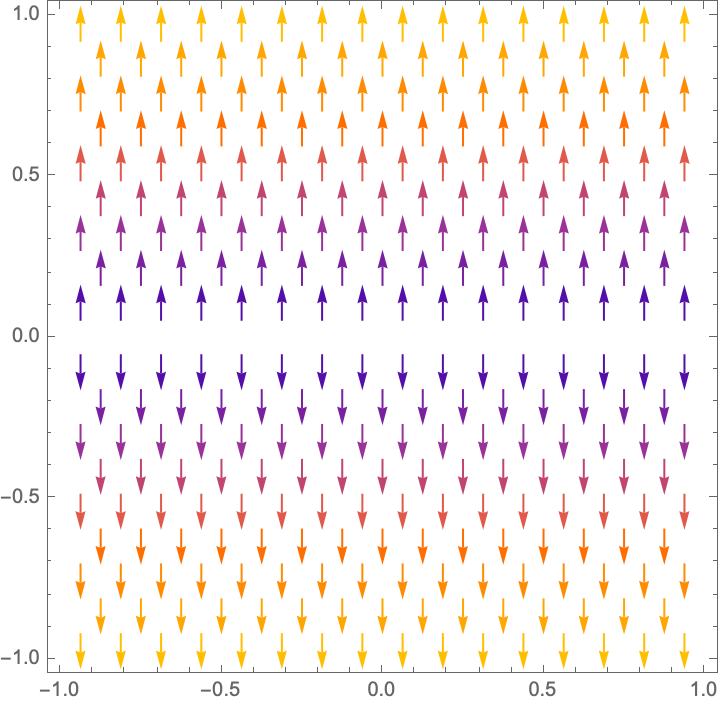
\includegraphics[width=0.9\linewidth]{fig6}
				\caption*{$V$}
			\end{subfigure}
			\begin{subfigure}{0.5\linewidth}
				\centering
				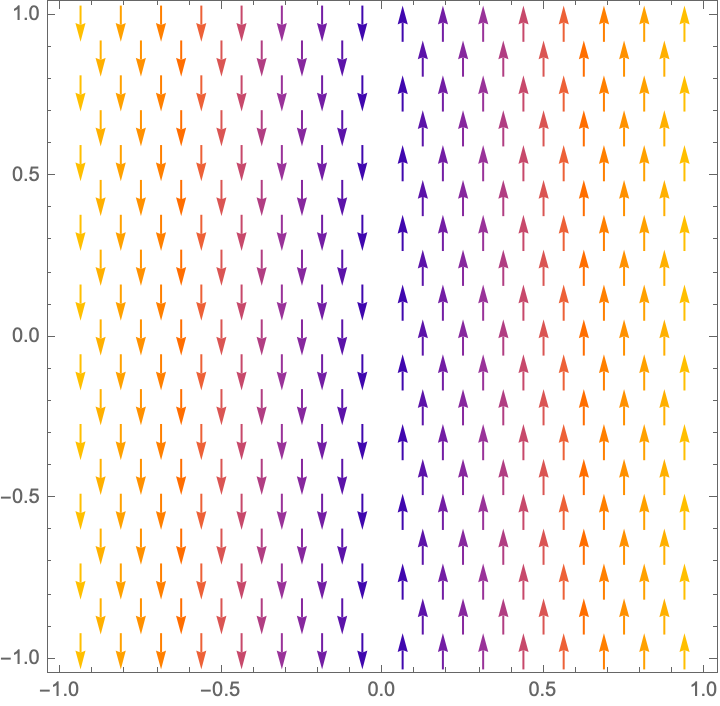
\includegraphics[width=0.9\linewidth]{fig7}
				\caption*{$W$}
			\end{subfigure}
		\end{figure}
		En este caso podemos describir explícitamente el flujo de $V$ como la función
		\[(t,x_0,y_0)\mapsto\psi(t,x_0,y_0):=(x(t),y(t))\]
		Que satsiface el sistema de ecuaciones diferenciales
		\[\begin{pmatrix}
			\frac{dx}{dt}\\
			\frac{dy}{dt}
		\end{pmatrix}=
		\begin{pmatrix}
			0\\
			y
		\end{pmatrix}\]
		cuyas soluciones son $x(t)=x_0$, $y(t)=y_0e^t$.
		
		La función que "regresa" $t$ unidades de tiempo a lo largo de una curva integral que pasa por el punto $(x,y)$ es $\psi_{-t}(x,y)=(x,ye^{-t})$. Al ser una función de $\R^2$ en sí mismo, su diferencial es una transformación lineal que se puede expresar mediante la matriz
		\[d(\psi_{-t})_{(x,y)}=\begin{pmatrix}
			1&0\\
			0&e^{-t}
		\end{pmatrix}\]
		de forma que envía $W_{(x,y)}=\begin{pmatrix}0\\x\end{pmatrix}\mapsto\begin{pmatrix}0\\xe^{-t}\end{pmatrix}$. Para aplicar nuestro teorema, vemos esta correspondencia como una función $F(t)$, cuya derivada es justamente el límite que escribimos arriba. Hemos confirmado que
		$F'(t)=\begin{pmatrix}
			0\\-xe^{-t}
		\end{pmatrix}=[V,W]=-W$.
		\begin{figure}[H]
			\centering
			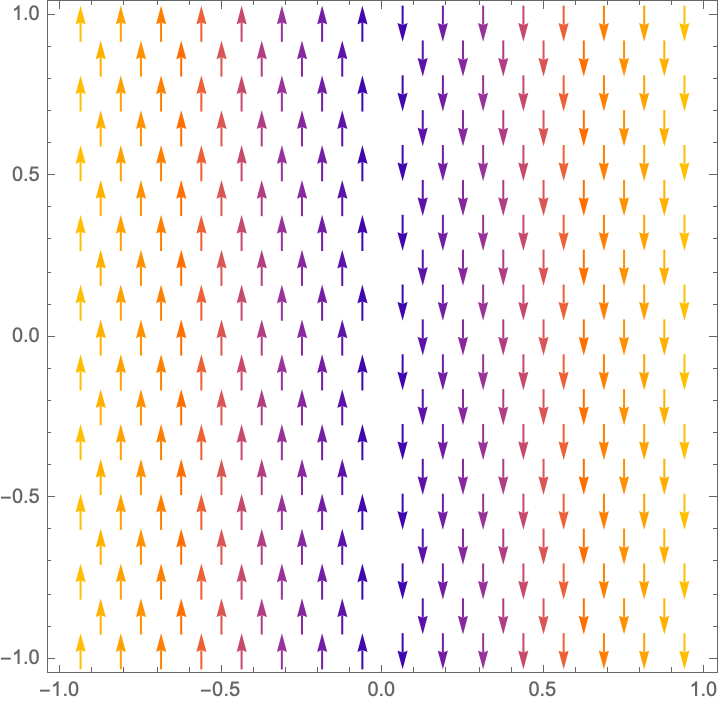
\includegraphics[width=0.45\linewidth]{fig8}
			\caption*{$-W$}
		\end{figure}
	\end{ejem}
	\begin{obs}[Corchete de Lie en coordenadas]
		Supongamos que $V=\sum_ia_i\frac{\partial}{\partial x^i}$ y $W=\sum_jb_j\frac{\partial}{\partial x^j}$, busquemos una expresión para las funciones $c_k$ en la expresión \[[V,W]=\sum_kc_k\frac{\partial}{\partial x^k}\]
		Para cualquier $f\in\Cinf(M)$,
		\begin{align*}
			[V,W](f)&=V(Wf)-W(Vf)\\
			&=V\left(\sum_jb_j\frac{\partial f}{\partial x^j}\right)-W\left(\sum_ia_i\frac{\partial f}{\partial x^i}\right)\\
			&=\sum_ia_i\frac{\partial }{\partial x^i}\left(\sum_jb_j\frac{\partial f}{\partial x^j}\right)-\sum_jb_j\frac{\partial }{\partial x^i}\left(\sum_ia_i\frac{\partial f}{\partial x^i}\right)\\
			&=\sum_i\sum_j\frac{\partial}{\partial x^i}\left(b_j\frac{\partial f}{\partial x^j}\right)-\sum_j\sum_i\frac{\partial}{\partial x^j}\left(a_i\frac{\partial f}{\partial x^i}\right)\\
			&=\ldots\\
			&=\sum_{i,j}\left(a_i\frac{\partial b_j}{\partial x^i}-b_j\frac{\partial a_i}{\partial x^j}\right)\frac{\partial f}{\partial x^j}
		\end{align*}
	\end{obs}
	\subsection{Ejercicios 4-8 septiembre}
	\begin{ejer}
		En $\R^3$ considera los campos vectoriales en coodenadas cartesianas $X=x^2E_1+yE_3$ y $Y=y^3E_2$ y la función $f:\R^3\to\R$ dada por $f(p,q,r)=p^2qr$. Calcula $[X,Y]$ en $(1,01)$, $fY$ en $(1,01)$ y $Yf$ en $(1,0,1)$. Expresa $X$ en términos de la base de campos coordenados correspondiente a coordenadas cilíndricas.
	\end{ejer}
	\begin{proof}[Solución]
		
		El corchete de Lie de $X$ y $Y$ debe ser un campo vectorial, es decir, un operador que asocia funciones suaves en la variedad con números reales. Para cualquier $g\in\Cinf(\R^3,\R)$, tenemos
		\begin{align*}
			[X,Y](g)&=X(\underbrace{Yg}_{\in\Cinf(\R^3,\R)})-Y(\underbrace{Xg}_{\in\Cinf(\R^3,\R)})\\
			&=\ldots\\
			&=-y^3\frac{\partial g}{\partial z}\in\R
		\end{align*}
		Es decir, $[X,Y]=-y\frac{\partial}{\partial z}$, de forma que $[X,Y]_{(1,0,1)}=-0\frac{\partial}{\partial z}\in T_{(1,0,1)}\R^3$.
		
		Luego, $fY$ también es un campo vectorial, así que al evaluar en punto nos da un vector tangente:
		\[(fY)_{(1,0,1)}=f(1,0,1)(y^3E_2)_{(1,0,1)}=0\in T_{(1,0,1)}\R^3\]
		Por otro lado, $Yf$ es una función definida en la variedad $\R^3$ que en cada punto nos devuelve un número real:
		\[(Yf)(1,0,1)=\left[y^3\frac{\partial f}{\partial y}\right]_{(1,0,1)}=[y^3x^2z]_{(1,0,1)}=0\in\R\]
		
		El mapeo $T:\R^3\to\R^3$ que cambia coordenadas cilíndricas a cartesianas manda $(r,\theta,z)\mapsto(r\cos\theta,r\sen\theta,z)$. Su diferencial
		\[dT=\begin{pmatrix}
			\cos\theta&-r\sen\theta&0\\
			\sen\theta&r\cos\theta&0\\
			0&0&1
		\end{pmatrix}\]
		tiene inversa
		\[dT^{-1}=\begin{pmatrix}
			\cos\theta&\sen\theta&0\\
			-\frac{1}{r}\sen\theta&\frac{1}{r}\cos\theta&0\\
			0&0&1
		\end{pmatrix}.\]
		Los vectores columna de $dT^{-1}$ son las coordenadas cilíndricas de los vectores tangentes básicos $E_1$, $E_2$ y $E_3$. Sustituyendo,
		\begin{align*}
			X&=r^2\cos^2\theta(\cos\theta E_r-\frac{1}{r}\sen\theta E_\theta)+r\sen\theta E_z\\
			&=r^2\cos^3\theta E_r-r\cos^2\theta\sen\theta E_\theta+r\sen\theta E_z.
		\end{align*}
		También se puede definir el cambio de coordenadas normalizando los vectores.
	\end{proof}
	\begin{figure}[H]
		\begin{subfigure}{0.5\linewidth}
			\centering
			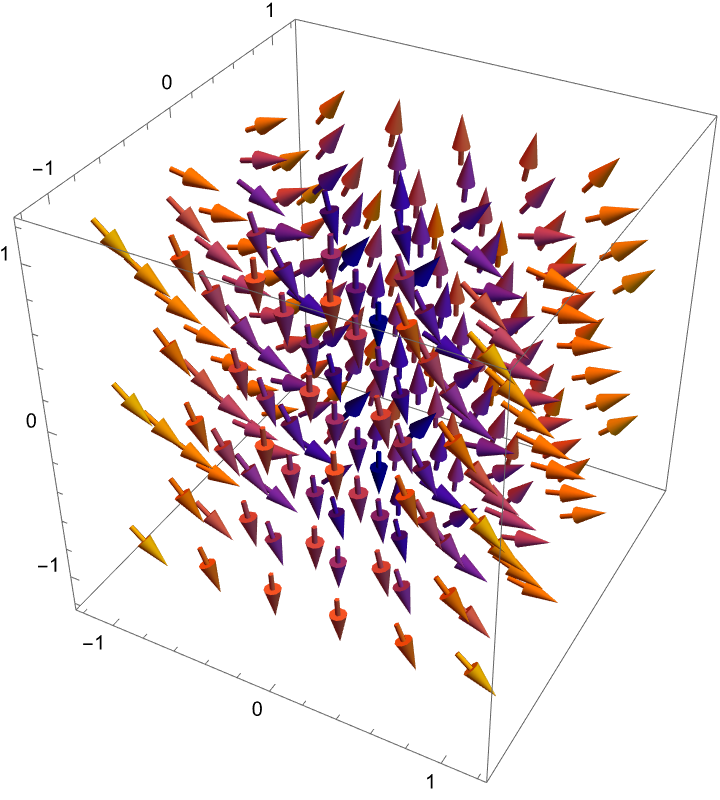
\includegraphics[width=0.9\linewidth]{fig10}
			\caption*{$X$}
		\end{subfigure}
		\begin{subfigure}{0.5\linewidth}
			\centering
			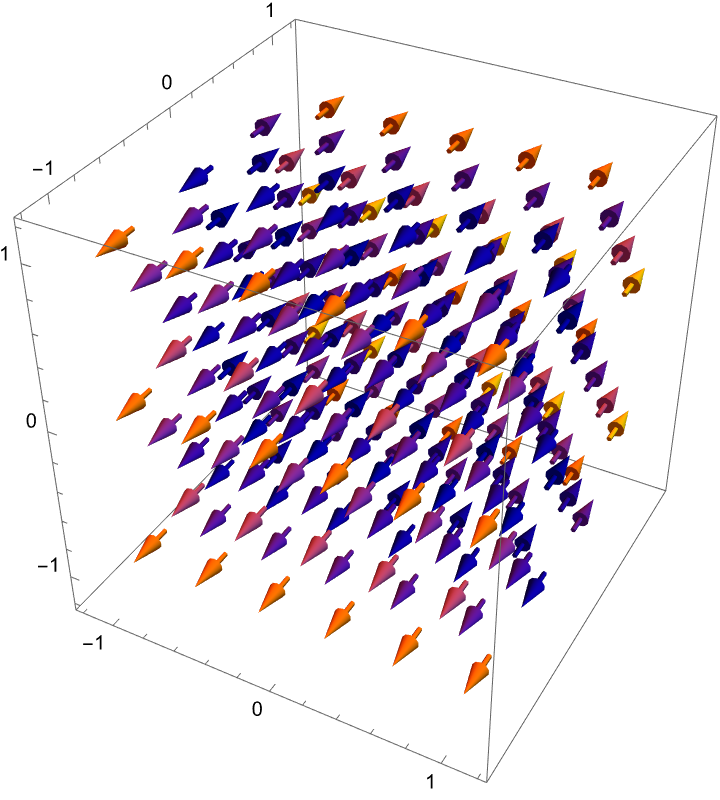
\includegraphics[width=0.9\linewidth]{fig11}
			\caption*{$Y$}
		\end{subfigure}
		\begin{center}
			\begin{subfigure}{0.5\linewidth}
				\centering
				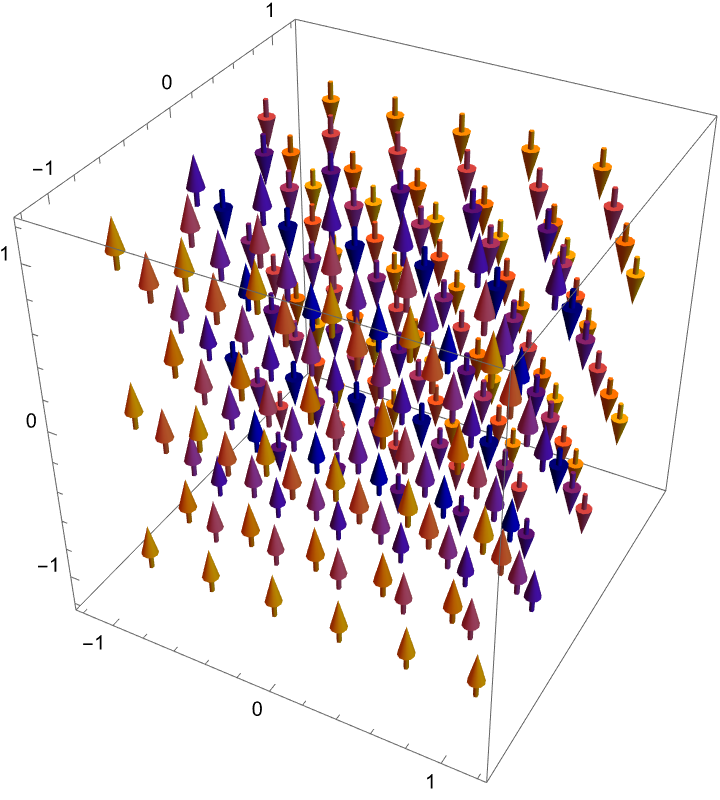
\includegraphics[width=0.9\linewidth]{fig12}
				\caption*{$[X,Y]$}
			\end{subfigure}
		\end{center}
	\end{figure}
	
	\section{Teorema de rectificación}
	Podemos simplificar la expresión local de un campo vectorial mediante un cambio de coordenadas:	
	\begin{lema}[\cite{ONeill}\textbf{, 57}]
		Si $V$ es un campo vectorial y $p\in M$ con $V_p\neq0$, entonces existe un sistema de coordenadas $x^1,\ldots,x^n$ alrededor de $p$ tal que $V=\frac{\partial}{\partial x^1}$.
	\end{lema}
	\begin{proof}
		Sea $\psi:I\times U\to M$ el flujo local de $V$ alrededor de $p$ relativo a la carta $h:U\to\R^n$. Tomemos un hiperplano en $\R^n$ que no contenga a $V_p$. Para fijar ideas, consideremos en el hiperplano normal $H$ a $V_p$. Entonces, $S:=h^{-1}(H)$ es una subvariedad. Usaremos la siguiente observación:
		\begin{obs}
			Podemos ver el espacio tangente de una subvariedad como subespacio del espacio tangente de la variedad. Aunque esto no es formalmente cierto, para $w\in T_pS$ podemos asociarle el vector $dj_p(w)\in T_pM$ que manda $g\in\Cinf(M,\R)\mapsto w(g|_S)$. (Ver \cite{Lee}, 5.37).
		\end{obs}
		Ahora restrinjamos el flujo a la subvariedad, y tomemos $q\in S\cap U$. El flujo es un difeomorfismo entre $J\times V$ (ver O'Neill). Para un sistema de coordenadas $z^2(q),\ldots,z^n(q)$ en la subvariedad, tenemos coordenadas $x^1(r)=t,x^2(r)=z^2(q),\ldots x^n(r)=z^n(q)$ en $ J\times V$. Estas coordenadas se pueden tomar como coordenadas de $M$, para las cuales $V=\frac{\partial}{\partial x^1}$. Para verlo, tomamos una curva integral $\alpha$ de $V$ de forma que $V(x^1)=(\frac{d}{dt}x^1(\alpha(t)))=\frac{dt}{dt}=1$, y en las demas coordenadas se anula por no depender de $t$.
	\end{proof}
	Ahora comparemos con las ideas de Arnold en su libro de ecuaciones diferenciales ordinarias:
	\begin{defn}[\cite{Arnold}]
		Un \textbf{campo de direcciones en $\R^n$} es una función que a cada punto le asocia una recta que pasa por ese punto.
		
		Una \textbf{rectificación} de un campo de direcciones en $\R^n$ es un difeomorfismo que lo transforma en un campo de direcciones paralelas. Un campo de direcciones es \textbf{rectificable} si existe una rectificación de él.
	\end{defn}
	\begin{teo}
		Todo campo de direcciones suave es rectificable en una vecindad de cada punto.
	\end{teo}
	\begin{teo}
		La ecuación diferencial $\dot{x}=v(t,x)$ con $v$ suave es localmente equivalente a la ecuación $\frac{dy}{dz}$ $\frac{dy}{dz}=0$ mediante el cambio de coordenadas $(t,x)\leftrightarrow(y,z)$.
	\end{teo}
	\begin{ejer*}[\cite{Lee}\textbf{, 9.5}]
		Supongamos que $M$ es una variedad suave y compacta que admite un campo vectorial que no se anula en ninguna parte. Demuestre que existe un mapeo suave $F:M\to M$ que es homotópico a la identidad y no tiene puntos fijos.
	\end{ejer*}
	\begin{proof}[Solución]
		La idea es tomar el flujo del campo vectorial y fijar una $t_0$ tal que al avanzar $t_0$ unidades de tiempo no quede ningún punto fijio.
		
		Supongamos que $V$ es un campo vectorial que no se anula en ninguna parte, de forma que para cualquier punto $p\in M$ podemos encontrar una vecindad $U_p$ donde $V=\frac{\partial}{\partial x^1}$ para las coordenadas $h=(x^1,\ldots,x^n)$ en $U_p$. Una curva integral $\alpha$ de $V$ tiene coordenadas $(t,0,\ldots,0)$, ya que su derivada manda $f\in\Cinf\mapsto\frac{d}{dt}f\circ\alpha=\frac{\partial (f\circ h^{-1})}{\partial x^1}$.
		
		Hemos construido una cubierta abierta $\{U_p\}_{p\in M}$ de $M$, que tiene una subcubierta finita $U_1,\ldots, U_k$. ¿Cómo nos aseguramos de que hay una $t_0$ tal que el flujo $\psi_{t_0}:M\to M$ no se salga del dominio de todos estos abiertos?
		
		Conviene hacer con un poco más de detalle la construcción: en vez de aplicar la compacidad a la cubierta $\{U_p\}$, debemos tomar una bola de radio $\varepsilon_p$ dentro de cada abierto $h(U_p)\subset\R^n$ (donde el flujo tiene la expresión que hemos especificado). Y ahora sí, la cubierta de "bolas" $\{h^{-1}(B_{\varepsilon_p/2}(h(p)))\}_{p\in M}$ tiene una subcubierta finita $\{h^{-1}(B_{\varepsilon_i/2}(h(p_i)))\}_{i=1}^k$ y podemos definir $t_0:=\min_{1\leq i\leq k}\varepsilon_i/2$. (Hemos tomado $\varepsilon_p/2$ para asegurarnos de que la curva integral que pase por cualquier punto del abierto no se salga).
		
		Se sigue de la expresión local del flujo que la función suave $\psi_{t_0}:M\to M$ no tiene puntos fijos, y la homotopía $H:[0,1]\times M\to M$ que manda $(s,p)\mapsto \psi_{st_0}(p)$ es la buscada.
	\end{proof}
	¿Qué clase de información nos da este resultado? Para desarrollar intuición veamos un ejemplo.
	\begin{ejer*}[\cite{Lee}\textbf{, 9.4}]
		En $S^n\subset\C^{n+1}$ con $n$ impar, definamos $\theta(t,z)=e^{it}z$. Entonces, el \textbf{generador infinitesimal} de $\theta$, es decir, el campo vectorial $V_p=\frac{d}{dt}\theta(t,p)$, es un campo vectorial suave que no se anula.
	\end{ejer*}
	\begin{proof}
		Derivando respecto a $t$, obtenemos que $V_p=ie^{it}z$ como vector en $\C^{n+1}$. Es claro que este vector nunca se anula. Además, se trata de un campo vectorial suave simplemente por ser el generador infinitesimal de un flujo (Proposición 9.11).
	\end{proof}
	
	¿Será que si una variedad no admite un campo vectorial que no se anula en ninguna parte no es posible construir una función suave homotópica a la identidad y sin puntos fijos? Veamos el siguiente teorema de topología algebraica:
	\begin{teo}[de la bola peluda \cite{Hatcher}\textbf{, 2.28}]\label{teo:bola-peluda}
		$S^n$ admite un campo vectorial continuo que no se anula si y sólo si $n$ es impar.
	\end{teo}
	Así que en $S^2$, por ejemplo, cualquier campo vectorial suave se anula en por lo menos un punto. ¿Será que entonces no hay una función homotópica a la identidad y sin puntos fijos? Al menos en las esferas de dimensión par, la respuesta es que no.
	
	Cuando una función ${f:S^n\to S^n}$ no tiene puntos fijos, el segmento que une $f(x)$ y $-x$ no pasa por el origen, así que podemos definir la homotopía de la línea recta normalizada $H(t,x)=(tf(x)-(1-t)x)/|(tf(x)-(1-t)x)|$. Ésta resulta ser una homotopía entre $f$ y la función antípoda $-\Id$.
	
	El resultado clave de topología algebraica (que no podemos demostrar) es que hay un \textbf{invariante homotópico} que se llama \textbf{grado} para funciones entre esferas que asocia el número $(-1)^{n+1}$ a la función antípoda y el número $1$ a la identidad. Así que estos números deben coincidir. De hecho, la prueba del teorema de la bola peluda es precisamente construyendo una homotopía entre la identidad y la antípoda.
	
	\chapter{Formas y tensores}
	\section{Tensores}
	Éstas son las definiciones de \cite{ONeill}. También recomendamos consultar \cite{Palmas}. \textbf{Advertencia:} la notación en estos dos libros (y en otros) puede no ser igual.
	\begin{defn}[\cite{ONeill}\textbf{, Cap 3}]
		Para cuelesquiera espacios vectoriales (o más generalmente, módulos) $V_1,\ldots,V_s$, podemos definir el \textbf{producto directo} como el espacio vectorial definido con las operaciones naturales en $V_1\times\ldots\times V_s$. Si $V_1=\ldots=V_s$, denotamos este espacio vectorial por $V^s$.
		
		Una función definida en un espacio de este estilo es \textbf{multilineal} si es lineal en cada entrada.
	\end{defn}
	\begin{defn}
		Sea $V$ un espacio vectorial sobre un campo $K$. Un \textbf{$(r,s)$-tensor} es una función $K$-multilineal definida en el producto directo de $(V^*)^r$ con $V^s$. Es decir, es una función multilineal
		\[T:(V^*)^r\times V^s\to K\]
	\end{defn}
	
	Ahora comparemos con la definición de \cite{Spivak}:
	\begin{defn}
		Un $k$-tensor es una función multilineal
		\[T:V^k\to\R\]
	\end{defn}
	\begin{obs}
		El conjunto de $k$-tensores $\tau^k(V)$  tiene estructura de espacio vectorial con las operaciones
		\begin{align*}
			(S+T)(v_1,\ldots,v_k)=S(v_1,\ldots,v_k)+T(v_1,\ldots,v_k)\\
			(\lambda T)(v_1,\ldots,v_k)=\lambda T(v_1,\ldots,v_k)
		\end{align*}
	\end{obs}
	\begin{defn}
		Para  el \textbf{producto tensorial} de $S\in\tau^k(V)$ y $T\in\tau^\ell(V)$ es el tensor $S\otimes T\in\tau^{k+\ell}(V)$ dado por
		\begin{align*}
			S\otimes T:V^k\times V^\ell&\to\R\\
			(v_1,\ldots,v_k,v_{k+1},\ldots,v_{k+\ell})&\mapsto S(v_1,\ldots,v_k)\otimes T(v_{k+1},\ldots,v_{k+\ell})
		\end{align*}
	\end{defn}
	\begin{obs}[Intuición sobre el producto tensorial]
		El producto tensorial de dos espacios vectoriales $A$ y $B$ se puede pensar como el espacio vectorial donde viven los "productos" de los elementos de $A$ y $B$. Como en $\R^3$, no siempre es posible definir un producto entre vectores, así que esta estructura a menudo se "sale" de los espacios originales y resulta en un objecto algebraico abstracto.
	\end{obs}
	\begin{prop}
		Dada una base $v_1,\ldots,v_n$ de $V$, tenemos la base $\varphi_1,\ldots,\varphi_n$ del espacio dual $V*$ dada por
		\begin{align*}
			\varphi_i:V&\to\R\\
			v_j&\mapsto\delta_{ij}=\begin{cases}
				0\qquad\text{si }i\neq j\\
				1\qquad\text{si }i=j
			\end{cases}
		\end{align*}
		Entonces, los productos de la forma $\varphi_{i_1}\otimes\ldots\otimes\varphi_{i_k}$ son una base de $\tau^k(V)$.
	\end{prop}
	\begin{obs}\label{pullback}
		Dada una transformación lineal entre espacios vectoriales $f:V\to W$, tenemos la transformación lineal 
		\begin{align*}
			f^*:\tau^k(W)&\to\tau^k(V)\\
			T(v_1,\ldots,v_k)&\mapsto T(f(v_1),\ldots,f(v_k))
		\end{align*}
	\end{obs}
	\begin{defn}
		Un $k$-tensor $T$ en $V$ es \textbf{alternante} si
		\[T(v_1,\ldots,v_i,\ldots,v_j,\ldots,v_k)=-T(v_1,\ldots,v_j,\ldots,v_i,\ldots,v_k)\]
		Y denotaremos al conjunto de $k$-tensores alternantes por $\Lambda^k(V)$.
	\end{defn}
	Para $T\in\tau^k(V)$, definamos
	\[	\Alt(T)=\frac{1}{k!}\sum_{\sigma\in S_k}\sgn\sigma T(v_{\sigma(1)},\ldots,v_{\sigma(k)})\]
	\begin{prop}\leavevmode
		\begin{enumerate}
			\item Si $T\in\tau^k(V)$, entonces $\Alt(T)\in\Lambda^k(V)$.
			\item Si $\omega\in\Lambda^k(V)$, entonces $\Alt(\omega)=\omega$.
			\item  Si $T\in\tau^k(V)$, entonces $\Alt(\Alt(T))=\Alt(T)$.
		\end{enumerate}
	\end{prop}
	El producto tensorial de dos tensores alternantes no necesariamente es alternante, por lo que definimos
	\begin{defn}
		El \textbf{producto cuña} de dos tensores alternantes $\omega\in\Lambda^k(V)$ y $\eta\in\Lambda^\ell(V)$ es 
		\[\omega\wedge\eta=\frac{(k+\ell)!}{k!\ell!}\Alt(\omega\otimes\eta)\]
	\end{defn}
	\begin{prop}[Propiedades del producto cuña]\leavevmode
		\begin{enumerate}
			\item $(\omega_1+\omega_2)\wedge\eta=\omega_1\wedge\eta+\omega_2\wedge\eta$.
			\item $\omega\wedge(\eta_1+\eta_2)=\omega\wedge\eta_1+\omega\wedge\eta_2$.
			\item $\lambda(\omega\wedge\eta)=\lambda\omega\wedge\eta=\omega\wedge\lambda\eta$.
			\item $\omega\wedge\eta=(-1)^{k\ell}\eta\wedge\omega$ \textbf{(Anticonmutatividad)}
			\item $f^*(\omega\wedge\eta)=f^*(\omega)\wedge f^*(\eta)$.
			\item $(\omega\wedge\eta)\wedge\theta=\omega\wedge(\eta\wedge\theta)$.
		\end{enumerate}
	\end{prop}
	\begin{prop}\label{prop:base-kth-exterior-power}
		La colección de formas alternantes $\varphi_ {i_1}\wedge\ldots\wedge\varphi_{i_k}$ con $1\leq i_1\leq\ldots\leq i_k\leq n$ es una base de $\Lambda^k(V)$, de forma que tiene dimensión $\binom{n}{k}$.
	\end{prop}
	\begin{prop}
		Sean $v_1,\ldots,v_k$ son una base de un espacio vectorial $V$ y $\omega\in\Lambda^n(V)$. Para los vectores $w_i=\sum_j\lambda_{ij}v_j$ en $V$, tenemos que
		\[\omega(w_1,\ldots,w_n)=\det(\lambda_{ij})\omega(v_1,\ldots,v_k)\]
	\end{prop}
	
	\section{Covectores}
	\begin{defn}
		Una \textbf{1-forma} (\textbf{covector}) en un espacio tangente $T_pM$ es una función lineal $\omega:T_pM\to\R$.
	\end{defn}
	Las 1-formas (covectores) son elementos en el dual del espacio tangente $T_pM^*$, que llamaremos el espacio \textbf{cotangente}.
	\begin{ejem}[Dos 1-formas en $(T_p\R^2)^*$]
		Dada una curva $\alpha:I\subset\R\to\R^2$ tal que $\alpha(0)=(x_0,y_0)$ y $\alpha'(0)=(v_1,v_2)$, tenemos las 1-formas (covectores)
		\begin{align*}
			\begin{aligned}
				dx:T_{(x_0,y_0)}\R^2&\to\R\\
				v=\alpha'(0)&\mapsto v_1
			\end{aligned}
			\qquad
			\begin{aligned}
				dy:T_{(x_0,y_0)}\R^2&\to\R\\
				v=\alpha'(0)&\mapsto v_1
			\end{aligned}
		\end{align*}
		Y resultará que cualquier $\omega\in T_(x_0,y_0)\R^2$ es de la forma $\omega=adx+bdy$. Es decir:
		\begin{align*}
			\omega:T_{(x_0,y_0)}\R^2&\to\R\\
			(v_1,v_2)&\mapsto av_1+bv_2
		\end{align*}
	\end{ejem}
	Ahora consideremos un vector tangente a una variedad $M$ en algún punto $p$ que en coordenadas locales se exprese como
	\[v_p=a_1(p)\frac{\partial}{\partial x^1}\Big|_p+\ldots+a_n(p)\frac{\partial}{\partial x^n}\Big|_p\]
	Si $\omega\in(T_pM)^*$, por linealidad tenemos
	\[\omega(v_p)=a_1(p)\omega\left(\frac{\partial}{\partial x^1}\Big|_p\right)+\ldots+a_n(p)\omega\left(\frac{\partial}{\partial x^n}\Big|_p\right)\]
	\begin{obs}
		Tendremos que
		\[dx_p^i\left(\frac{\partial}{\partial x^j}\Big|_p\right)=\begin{cases}
			1\qquad\text{si }i=j\\
			0\qquad\text{si }i\neq j
		\end{cases}\]
	\end{obs}
	\begin{obs}
		Las 1-formas (covectores) $dx^1,\ldots,dx^n$ son una base del espacio cotangente $(T_pM)^*$.
	\end{obs}
	\begin{obs}
		En el ejemplo anterior usamos que la derivada de una curva es un vector tangente. De hecho, otra forma de definir los vectores tangentes es justo como derivadas de curvas (ver \cite{DoCarmo} y \cite{Lee} \textbf{Prop 3.23}).
	\end{obs}
	
	\begin{obs}
		Las funciones bilineales de la forma $\omega:V\times W\to\R$ también forman un espacio vectorial. Si $V=W=\R^n$ tenemos como ejemplos determinante y el producto escalar.
	\end{obs}
	
	Ahora tratemos de definir una operación en el espacio cotangente, que llamaremos \textbf{producto cuña}. Consideremos el caso de una variedad de dimensión 2 $M$. Como en el caso de $M=\R^2$, los covectores $dx^1$ y $dx^2$ forman una base del espacio cotangente. Definamos
	\[dx^1\wedge dx^2:T_pM\times T_pM\to\R\]
	que actuará de la siguiente forma: para $u=a\frac{\partial}{\partial x^1}+b\frac{\partial}{\partial x^2}$ y $v=c\frac{\partial}{\partial x^1}+d\frac{\partial}{\partial x^2}$,
	\[(dx^1\wedge dx^2)(u,v)=\begin{bmatrix}
		a&b\\
		c&d
	\end{bmatrix}\]
	\section{Formas diferenciales}
	Ahora construimos el concepto dual al de campo vectorial para covectores.
	\begin{defn}
		Una \textbf{1-forma diferencial} en una variedad suave $M$ es una función que a cada punto $p\in M$ y a cada vector tangente $v_p\in T_pM$ le asocia un número $\omega(p,v_p)$.
	\end{defn}
	Localmente,
	\[\omega(p,v_p)=\sum_{i=1}^na_i(p)dx^i_p(v_p)\]
	con $a_i:U\subset M\to\R$ suave para toda $i$. Una expresión más sencilla es $\omega=\sum a_idx^i$.
	\begin{obs}
		Dado un campo vectorial $V$ y una 1-forma diferencial $\omega$ en $M$, podemos calcular
		\[p\mapsto V_p\mapsto\omega_p(V_p)\in\R\]
		Este número lo denotaremos, abusando de notación por
		\[\omega(V):M\to\R\]
	\end{obs}
	
	\section{Derivada exterior}
	Una función $f\in\Cinf(R^n,\R)$ se considera una 0-forma. Notemos que su diferencial $df$ es una 1-forma en cuanto a que para cualquier punto $p$ de la variedad, la función $df_p$ es un covector: a cada vector le asigna un número real. En coordenadas, tenemos
	\[df=\sum\frac{\partial f}{\partial x^i}dx^i\]
	
	La siguiente definición generaliza esta idea.
	\begin{defn}[\cite{Loring}\textbf{, 4.5}]
		Para una $k$-forma definida en algún abierto $U$ de $\R^n$,
		\[\omega=\sum_{1\leq i_1\leq\ldots\leq i_k\leq n}\omega_{ i_1,\ldots, i_k}dx_{i_1}\wedge\ldots\wedge dx_{i_k}:=\sum_Ia_Idx^I\]
		su \textbf{derivada exterior} o \textbf{diferencial} es la $(k+1)$-forma
		\[d\omega=\sum_Ida_I\wedge dx^I=\sum_I\left(\sum_j\frac{\partial a_I}{\partial x^j}dx^j\right)\wedge dx^I\]
	\end{defn}
	\begin{defn}\leavevmode
		\begin{itemize}
			\item 		Una $k$-forma $\omega$ es \textbf{cerrada} si $dw=0$
			\item Una $k$-forma es \textbf{exacta} si existe una $(k-1)$-forma $\theta$ tal que $\omega=d\theta$.
		\end{itemize}
	\end{defn}
	\begin{prop}[\cite{Loring}\textbf{, 4.7}] Si $U$ es un abierto de $\R^n$
		\begin{enumerate}
			\item $d^2=0$. (Usando la conmutativadad de las segundas derivadas parciales)
			\item Si $f\in\Cinf(U,\R)$, y $X\in\mathfrak{X}(U)$, $(df)(X)=Xf$.
		\end{enumerate}
	\end{prop}
	\begin{ejem}[Una 1-forma cerrada que no es exacta, \cite{Loring}\textbf{, 4.9 y ejemplo p. 43}]
		Consideremos la 1-forma 
		\[\omega=\frac{-y}{x^2+y^2}dx+\frac{x}{x^2+y^2}dy\]
		definida en $\R^2-\{0\}$. Una 1-forma $Pdx+Qdy$ es cerrada cuando $\frac{\partial P}{\partial y}=\frac{\partial Q}{\partial x}$, así que $\omega$ es cerrada. Consideremos la integral
		\[\int_\alpha\omega=\int_0^{\theta_0}-\sen t(-\sen t)+\cos t\cos tdt=\int_0^{\theta_0}dt=\theta_0\]
		
		Para ver que $\omega$ no es exacta, supongamos que $f:\R^2-\{0\}\to\R$ es tal que $df=\omega$. En este caso, sabemos que la integral de línea sobre cualquier curva cerrada debe dar cero. Explícitamente, si $\alpha(t)=(\cos(t),\sen(t))$,
		\begin{align*}
			\int_\alpha\omega&=\int_0^{\theta_0}\frac{\partial f}{\partial x}(x(t),y(t))\frac{dx}{dt}+\frac{\partial f}{\partial y}(x(t),y(t))\frac{dy}{dt}dt\\
			&=\int_0^{\theta_0}\frac{d}{dt}f(x(t),y(t))dt\\
			&=f(x(\theta_0),y(\theta_0))-f(x(0),y(0))\\
			&=f(\cos\theta_0,\sen\theta_0)-f(1,0)
		\end{align*}
		Haciendo $\theta_0\to2\pi$ esta integral tiende a $0$, pero la anterior tiende a $2\pi$.
	\end{ejem}
	
	Resulta que la proporción de formas exactas respecto a formas cerradas depende exclusivamente de la topología de una variedad. Siguiendo a \cite{Loring}, definamos el cociente de dos espacios vectoriales
	\[H^k(U)=\frac{\{k\text{-formas cerradas en }M\}}{\{k\text{-formas exactas en }M\}}\]
	que llamaremos la \textbf{$k$-ésima de cohomología de De Rham} de $M$, que está bien definido ya que cualquier forma cerrada es exacta. Georges De Rham demostró en 1931 que las formas diferenciales satisfacen los mismos axiomas que los ciclos y las cadenas de la homología singular, mostrando una dualidad entre estas construcciones.
	
	Un resultado central en esta teoría es que dos espacios homotópicamente equivalentes tienen asociada la misma cohomología (Corolario 27.11). En particular, como $\R^n$ es contraíble (homotópicamente equivalente a un punto), su cohomología es trivial para $k\geq1$: ¡no hay 1-formas no triviales definidas en el espacio unipuntual! Este resultado se conoce como el Lema de Poincaré (Corolario 27.13).
	
	En el ejemplo anterior vimos un espacio no contraible cuya primera homología no es trivial: hay una 1-forma cerrada que no es exacta.
	
	Mostramos una demostración "a pie" del Lema de Poincaré para subconjuntos estrellados de $\R^n$ (en particular, todo $\R^n$). Un conjunto $U\subset \R^n$ es \textbf{estrellado} si existe un punto $c$ tal que para cualquier $x\in U$ el segmento que une $c$ y $x$ se queda contenido en $U$.
	
	\begin{teo}[\cite{Lee}\textbf{, 11.49, Lema de Poincaré para conjuntos estrellados}]
		Cualquier 1-forma cerrada definida en un conjunto estrellado $U\subseteq\R^n$ es exacta.
	\end{teo}
	\begin{proof}
		Sea $\omega$ una 1-forma cerrada en $U$. Supongamos sin pérdida de generalidad que el centro de $U$ es el origen (la traslación adecuada manda formas cerradas en cerradas y exactas en exactas). Mostraremos que
		\[d\int_{\gamma_x}\omega=\omega\]
		donde $\gamma_x(t)=tx$ para $0\leq t\leq1$, el segmento que une $x$ al origen.
		
		Supongamos que $\omega=\sum_{i=1}^n\omega_idx^i$. Como la integral es una función real-valuada en $U$, para encontrar su derivada exterior basta encontrar sus derivadas parciales:
		\begin{align*}
			\frac{\partial}{\partial x^j}\int_{\gamma_x}\omega(x)&=\frac{\partial}{\partial x^j}\int_0^1\sum_{i=1}^n\omega_i(tx)x^idt\\
			&=\int_0^1\sum_{i=1}^n\frac{\partial}{\partial x^j}\omega_i(tx)x^idt\\
			&=\int_0^1\left(\sum_{i=1}^n\frac{\partial \omega_i}{\partial x^j}(tx)tx^i+\omega_j(tx)\right)dt\\
			&=\int_0^1\left(\sum_{i=1}^n\frac{\partial \omega_j}{\partial x^i}(tx)tx^i+\omega_j(tx)\right)dt\\
			&=\int_0^1\frac{d}{dt}t\omega_{j}(tx)dt\\
			&=\omega_j(x)
		\end{align*}
		Usando que como $\omega$ es cerrada,
		\[\frac{\partial \omega_i}{\partial x^j}=\frac{\partial \omega_j}{\partial x^i}\]
	\end{proof}
	\section{Variedades orientables y no orientables}
	En un espacio vectorial $V$ de dimensión finita definamos una relación de equivalencia entre bases $\{v_1,\ldots,v_n\}\sim\{w_1,\ldots,w_n\}$ cuando el determinante de la transformación lineal $T:V\to V$ tal que $T(v_j)=w_j$ para toda $j$ es positivo.
	
	\begin{defn}[\cite{DoCarmo}\textbf{, 4.4}]
		Una variedad diferenciable $M$ es \textbf{orientable} si admite un atlas $A$ para el cual los cambios de coordenadas tienen jacobiana con determinante positivo. La elección de tal estructura diferenciable se llama \textbf{orientación}, y una \textbf{variedad orientada} es una pareja $(M,A)$. Dos orientaciones cuya unión es un atlas para el cual los cambios de coordenadas tienen jacobian con determinante positivo \textbf{determinan la misma orientación}.
	\end{defn}
	\begin{obs}\leavevmode
		\begin{itemize}
			\item Si $M$ es orientable y conexa entonces existen exactamente dos orientaciones distintas.
			\item Si $M$ y $N$ son difeomorfas, basta que una sea orientable para que la otra lo sea.
			\item Si $M$ y $N$ son variedades difeomorfas orientadas, un difeomorfismo puede \textbf{preservar} o \textbf{invertir} la orientación. Explícitamente, si $\varphi:(M,A)\to (N,B)$ es un difeomorfismo entre variedades orientables, $\varphi$ induce un atlas $B'$ en $N$ como sigue: para una carta coordenada $h:U\subset M\to\R^n$ definimos $\varphi\circ h^{-1}:\R^n\to \varphi(U)$. Cuando $B$ y $B'$ determinan la misma orientación decimos que $\varphi$ preserva orientación.
			\item Si $M$ puede ser cubierta por dos vecindades coordenadas cuya intersección es conexa, entonces $M$ es orientable. El determinante de la Jacobiana del cambio de coordenadas no puede ser 0 por tratarse de una función invertible. Como la intersección de las vecindades coordenadas es conexa, el determinante no puede cambiar de signo. Reajustando si es necesario las coordenadas, podemos suponer que el determinante es siempre positivo.
		\end{itemize}
	\end{obs}
	\begin{ejem}[$S^n$ es orientable]
		Consideremos el caso de $S^2$ con el atlas dado por las proyecciones estereográficas desde los polos norte y sur:
		\begin{align*}
			\begin{aligned}
				h_1:S^1\backslash\{N\}&\to\R^2\\
				(x,y,z)&\mapsto\left(\frac{x}{1-z},\frac{y}{1-z}\right)
			\end{aligned}\qquad\qquad
			\begin{aligned}
				h_2:S^1\backslash\{S\}&\to\R^2\\
				(x,y,z)&\mapsto\left(\frac{x}{1+z},\frac{y}{1+z}\right)
			\end{aligned}
		\end{align*}
		¿Cuál es la función de cambio de coordenadas $(u^1,v^1)\mapsto(u^2,v^2)$?
		\[u^2=\frac{u^1}{|(u^1,v^1)|^2}\qquad\qquad v^2=\frac{v^1}{|(u^1,v^1)|^2}\]
		Observemos que esta transformación fija la circunferencia unitaria en $\R^2$, e invierte las regiones de adentro y afuera. De hecho, se trata de la inversión respecto a la circunferencia unitaria. Como la intersección de estas dos vecindades es conexa, por la observación anterior $S^2$ (y con un argumento análogo $S^n$) es orientable.
	\end{ejem}
	\begin{obs}\label{obs:antipoda-orientacion}
		La transformación antípoda $-\Id:S^n\to S^n$ preserva la orientación cuando $n$ es impar, y la invierte cuando $n$ es impar. (Ver \hyperref[teo:bola-peluda]{Teorema de la bola peluda}). \href{https://math.stackexchange.com/questions/74712/proving-rigorously-a-map-preserves-orientation}{Esta} prueba me pareció buena, usando un campo normal. Otra idea para demostrarlo, siguiendo las ideas de \cite{Hatcher}, es ver la antípoda como la composición de tantas reflexiones como coordenadas en $\R^{n+1}$.
	\end{obs}
	\subsection{Ejercicios 14 de septiembre}
	\begin{defn}
		Se dice que un grupo $G$ \textbf{actúa} en una variedad difernciable $M$ si existe $\phi:G\times M\to M$ tal que
		\begin{itemize}
			\item Para cada $g\in G$ la transgormación $\phi_g:M\to M$ dada por $\phi_g(p)=\phi(g,p)$ es un difeomorfismo y $\phi_e:M\to M$ es la identidad en $M$.
			\item Si $g_1,g_2\in G$, entonces $\phi_{g_1g_2}=\phi_{g_1}\circ\phi_{g_2}$.
		\end{itemize}
		Por brevevedad escribiremos $gp$ para denotar $\phi(g,p)$.
		
		Diremos que la acción es \textbf{propiamente discontinua} si todo punto $p\in M$ tiene una vecindad $U\subset M$ tal que $U\cap g(U)\neq\varnothing$ para toda $g\neq e$.
	\end{defn}
	Una acción determina una relación de equivalencia en $M$ dada por $p\sim q$ si $p=gq$ para alguna $g\in G$.
	
	Denotando $M/G$ al espacio cociente relacionado a esta relación de equivalencia, tenemos la proyección natural $\pi:M\to M/G$. Para cada parametrización local ${\psi:\Omega\subset\R^n\to U\subset M}$ tenemos una función $\pi\circ\psi:\Omega\subset\R^n\to\pi(U)\subset M/G$.
	\begin{enumerate}
		\item Muestra que $M/G$ con estas parametrizaciones es una variedad diferenciable.
		\item Sea $M=S^2$ la esfera unitaria. Sea $G$ el grupo generado por la transformación atntípoda. ¿Qué variedad es $M/G$?
		\item Sea $M$ el cilindro infinito dado por los puntos $(x,y,z)$ tales que $x^2+y^2=1$ y $z\in\R$. Sea $G$ el grupo generado por $A:M\to M$, $A(x,y,z)=(-x,-y,-z)$. ¿Qué variedad es $M/G$?
		\item Prueba que $M/G$ es orientable si y sólo si existe una orientación de $M$ tal que es preservada por todo difeomorfismo de $G$.
		\item Prueba que las dos variedades anteriores son no-orientables.
	\end{enumerate}
	\begin{proof}[Solución]\leavevmode
		\begin{enumerate}
			\item Dada una parametrización local $\psi:\Omega\subset\R^n\to U\subset M$, podemos suponer que $U$ es tal que $U\cap g(U)\neq\varnothing$ para $g\in G$ con $g\neq e$ tomando la intersección si es necesario. Esto implica que $\pi|_U$ es inyectiva, y como además su imagen es un abierto (la proyección cociente es abierta), la familia de funciones $\pi\circ\psi$ definidas de esta forma son homeomorfismos de subconjuntos abiertos de $\R^n$ en subconjuntos abiertos de $M/G$ que cubren a $M/G$.
			
			Para ver que $M/G$ es una variedad diferenciable basta ver que los cambios de coordenadas son suaves. Sean $\pi\circ\psi_1$ y $\pi\circ\psi_2$ dos cartas en $M/G$ cuyos dominios $\pi(U_1)$ y $\pi(U_2)$ definidos como en el párrafo anterior tienen intersección no vacía. Los cambios de coordenadas son de la forma
			\begin{equation}\label{ec:cambio-coord-traslacion}
				(\pi\circ\psi_2)^{-1}\circ(\pi\circ\psi_1):\R^n\to\R^n
			\end{equation}
			Como $(\pi\circ\psi_2)^{-1}=\psi^{-1}\circ\pi|_{U_2}^{-1}$, basta demostrar que la función $\pi|_{U_2}^{-1}\circ\pi:M\to M$ es suave, pero esta función es justamente un difeomorfismo de $G$, que es suave por hipótesis.
			\[\begin{tikzcd}
				&\varnothing\neq\pi(U_1)\cap\pi(U_2)\subset M/G\\
				U_1\subset M\arrow[swap]{ur}{\pi|_{U_1}}&&U_2\subset M\arrow{ul}{\pi|_{U_2}}\\
				\Omega_1\subset\R^n\arrow{u}{\psi_1}&&\Omega_2\subset\R^n\arrow[swap]{u}{\psi_2}
			\end{tikzcd}\]
			
			\item El plano proyectivo $\R P^2$. Una recta por el origen en $\R^3$ tiene dos representantes en $S^2$, que se identifican cuando tomamos el cociente por el grupo generado por la transformación antípoda.
			
			\item Una banda de Möbius "infinita". En el caso de un cilindro acotado, digamos $\{(x,y,z)\in\R^3:x^2+y^2=1,|z|\leq1\}$, tenemos la siguiente situación (imagen de Andreo, es un \texttt{tikzpicture}?):
			\begin{figure}[H]
				\centering
				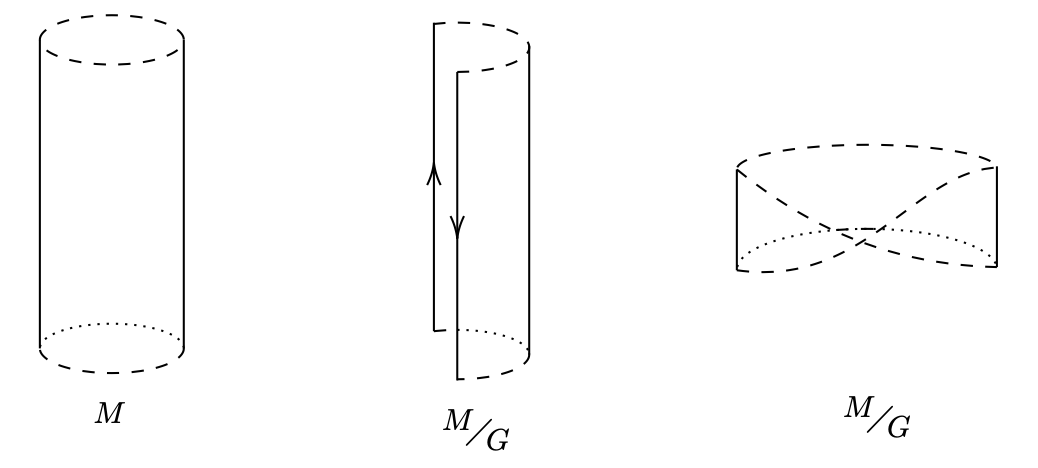
\includegraphics[width=0.7\linewidth]{fig13}
			\end{figure}
			
			\item Supongamos que $M/G$ es orientable. Entonces la jacobiana de los cambios de coordenadas como en \ref{ec:cambio-coord-traslacion} tiene determinante positivo, así que los difeomorfismos de $G$ también (cualquier difeomorfismo de $G$ se puede ver de esta forma).
			
			Al contrario, si la diferencial de cualquier difeomorfismo de $G$ tiene jacobiana con determinante positivo, es inmediato que los cambios de coordenadas en $M/G$ preservan orientación.
			
			\item Para el caso de $S^2$ ver la \hyperref[obs:antipoda-orientacion]{observación} anterior. Para el caso del cilindro se puede calcular explícitamente la jacobiana de la diferencial de la transformación antípoda y ver que su determinante es $-1$.
		\end{enumerate}
	\end{proof}
	
	\subsection{Más sobre orientaciones}
	Tanto en \cite{Lee} como en \cite{Loring} hay esencialmente tres maneras equivalentes de definir orientaciones en variedades diferenciables:
	\begin{enumerate}
		\item Existe un atlas tal que los cambios de coordenadas tienen jacobiana con determinante positiva. Hay dos posibles clases de equivalencia de tales atlases.
		\item Asignando primero una \textbf{orientación punto a punto} en los espacios tangentes de la variedad como espacios vectoriales, es decir, escogiendo una clase de equivalencia en las bases. Luego, escogiendo un \textbf{marco} (una colección de campos vectoriales $(E_1,\ldots,E_n)$ que en cada punto forman una base del espacio tangente) continuo tal que en cada punto forman una base que está en la clase de equivalencia distinguida.
		\item Existe una $n$-forma diferencial $\omega$ que no se anula. (Recordemos que el espacio de $n$-formas en una $n$-variedad es de dimensión 1). Una orientación es la elección de una de las dos posibles  clases de equivalencia de $n$-formas diferenciales en $M$ que no se anulan.
	\end{enumerate}
	Hay otra manera de definir orientaciones en variedades topológicas usando homología (\cite{Hatcher}, 3.3).
	
	\begin{ejer*}[\cite{Lee}\textbf{, 15.13}]
		Si $M$ y $N$ son variedades orientadas de dimensión $>0$ y ${F:M\to N}$ es un difeomorfismo local, son equivalentes:
		\begin{enumerate}
			\item La diferencial $dF_p$ envía bases orientadas (en la clase de equivalencia distinguida) de $T_pM$ en bases orientadas de $T_{F(p)}M$.
			\item Dadas dos cartas coordenadas cuyas bases canónicas $\frac{\partial}{\partial x^i}$ están en la clase de equivalencia distinguida, la diferencial de $F$ tiene jacobiana con determinante positivo.
			\item Dada una $n$-forma diferencial $\omega$ en $N$ que no se anula, la \textbf{forma inducida} o \textbf{pullback} $F^*\omega$ (definida \hyperref[pullback]{aquí}) está en la clase de equivalencia distinguida de $n$-formas diferenciales en $M$ que no se anulan.
		\end{enumerate}
	\end{ejer*}
	
	La condición 2 en este ejercicio es equivalente a la definición de \cite{DoCarmo} para que una función preserve orientación.
	
	Agregamos un resultado interesante:
	\begin{prop}[\cite{Lee-riem}\textbf{, 2.41. La forma Riemanniana de volumen}]
		
		Sea $(M,g)$ una variedad Riemanniana orientada de dimensión $n>1$. Entonces existe una única $n$-forma $dV$ en $M$ que llamaremos \textbf{forma de volumen} que satisface cualquiera de las siguientes propiedades equivalentes:
		
		\begin{enumerate}[label={(\arabic*)}]
			\item Si $(\varepsilon^1,...,\varepsilon^n)$ es cualquier \textbf{comarco} (campo de covectores que es una base de cada $T_pM^*$) ortonormal local orientado en $T^*M$, entonces
			\[dV=\varepsilon^1\wedge...\wedge\varepsilon^n\]
			\item Si $(E_1,...,E_n)$ es cualquier marco ortonormal local orientado de $TM$, entonces
			\[dV(E_1,...,E_n)=1\]
			\item Para cualesquiera cartas coordenadas locales orientadas $(x_1,...,x_n)$,
			$$dV=\sqrt{\det (g_{ij})}dx^1\wedge...\wedge dx^n$$
		\end{enumerate}
	\end{prop}
	
	
	%	\begin{lema}[\cite{Lee-intro-curv}\textbf{, 3.2}]
		%		En una variedad Riemanniana orientada existe una única $n$-forma $dV$ tal que $dV(E_1,\ldots,E_n)=1$ si $(E_1,\ldots,E_n)$ es un marco ortonormal orientado de $T_pM$ definido en algún $p\in M$. Esta forma se llama \textbf{elemento de volumen}.
		%	\end{lema}
	%	\begin{ejer*}[\cite{Lee-intro-curv}\textbf{, 3.9}]
		%		La expresión local de $dV$ respecto a cualquier marco local orientado $\{E_i\}$ es
		%		\[dV=\sqrt{\det g_{ij}}\varepsilon^n\wedge\ldots\wedge\varepsilon^n\]
		%		donde $g_{ij}=\langle E_i,E_j\rangle$ y $\{\varepsilon^i\}$ es el \textbf{comarco} dual (el campo de covectores en $T_pM^*$ canónico definido por $\varepsilon^i(E_j)=\delta^i_j$).
		%	\end{ejer*}
	
	
	\subsection{Más sobre variedades cociente}
	Es posible dar condiciones más generales para construir una variedad cociente con la acción de un grupo:
	
	\begin{teo}[\cite{Lee}\textbf{, 21.10}]
		Si $G$ es un \textbf{grupo de Lie} que actúa suave, \textbf{libre} y \textbf{propiamente} en una variedad suave $M$, el espacio de órbitas $M/G$ es una variedad topológica de dimensión $\dim M-\dim G$ y tiene una estructura diferenciable única tal que la proyección $\pi:M\to M/G$ es una sumersión suave.
	\end{teo}
	
	Un grupo de Lie $G$ es un grupo que además es una variedad diferenciable con la propiedad de que las funciones
	\begin{align*}
		\begin{aligned}
			G\times G&\to G\\
			(g,h)&\mapsto g\cdot h\\
		\end{aligned}
		\qquad\qquad\qquad
		\begin{aligned}
			G&\to G\\
			g&\mapsto g^{-1}\\
		\end{aligned}
	\end{align*}
	son suaves. Una acción es libre cuando no tiene puntos fijos, es decir, $gp\neq p$ para toda $g\neq e$. Por último, una acción es propia si el mapeo $G\times M\to M\times M$ dado por $(g,m)\mapsto (gm,m)$ es propio, es decir, la imagen inversa de un compacto es compacto.
	
	La condición de ser propia nos ayuda a descartar casos patológicos como el siguiente:
	\begin{ejem}[\cite{Lee}\textbf{, 21.3, Flujo irracional en el toro}]
		Para cualquier número irracional $\alpha$, el grupo aditivo $\R$ actúa en $\mathbb{T}=S^1\times S^1$ mediante
		\[t\cdot (w,z)=(e^{2\pi it}w,e^{2\pi i\alpha t}z)\]
		La órbita de cada punto es una curva densa, y de hecho el espacio de órbitas $\mathbb{T}/\R$ no es Housdorff: no podemos separar los puntos con abiertos.
	\end{ejem}
	\begin{prop}[\cite{Lee}\textbf{, 21.4}]
		Si un grupo de Lie actúa continua y propiamente en una variedad $M$, el espacio de órbitas es Housdorff.
	\end{prop}
	Por último incluimos el siguiente lema que nos recuerda a la definición de nuestros ejercicios:
	\begin{lema}[\cite{Lee}\textbf{, 21.11}]
		Supongamos que un grupo de Lie \textbf{discreto} $\Gamma$ actúa continua y libremente en una variedad $E$. La acción es propia si y sólo si se satisfacen las dos siguientes condiciones:
		\begin{enumerate}
			\item [\textit{(i)}] Cualquier punto $p\in E$ tiene una vecindad $U$ tal que para $(g\cdot U)\cap U=\varnothing$ a menos que $g=e$.
			\item [\textit{(ii)}] Si $p, p'\in E$ no están en la misma órbita, existen vecindades $V$ de $p$ y $V'$ de $p'$ tales que $(g\cdot V)\cap V'0\varnothing$ para toda $g\in\Gamma$.
		\end{enumerate}
	\end{lema}
	Un grupo de Lie es discreto si tiene la topología discreta, es decir, cualquier subconjunto es abierto.
	\section{Cambios de coordenadas}
	Consideremos un campo vectorial $X$ definido en alguna variedad $M$. Dadas dos vecindades coordenadas $U$ y $V$ con intersección no vacía, tenemos las expresiones
	\[X=\sum_{i=0}^na^i\frac{\partial}{\partial x^i}=\sum_{j=0}^nb^j\frac{\partial}{\partial y^j}\]
	y queremos encontrar la relación entre las funciones $a^i$ y $b^j$.
	
	Consideremos la matriz $M$ de la diferencial de $k\circ h^{-1}$, que es de la forma $M=\left(\frac{\partial y^j}{\partial x^i}\right)$. Observemos que $X(x^k)=a^k$, y $X(y^m)=b^m$. Y también $X(y^m)=\sum_{i=1}^na^i\frac{\partial y^m}{\partial x^i}$, así que de hecho
	\[\begin{pmatrix}
		\frac{\partial y^1}{\partial x^1}&\cdots&\frac{\partial y^m}{\partial x^n}\\
		\vdots&&\vdots\\
		\frac{\partial y^m}{\partial x^1}&\cdots&\frac{\partial y^m}{\partial x^n}\\
		\vdots&&\vdots\\
		\frac{\partial y^n}{\partial x^1}&\cdots&\frac{\partial y^n}{\partial x^1}
	\end{pmatrix}\begin{pmatrix}
		a^1\\\vdots\\a^n
	\end{pmatrix}=\begin{pmatrix}
		b^1\\\vdots\\ b^m\\\vdots\\b^n
	\end{pmatrix}\]
	dicho de otra forma, $Ma=b$.
	
	Ahora hagamos el mismo razonamiento para una 1-forma (pensada como una correspondencia que a cada punto de la variedad le asigna un elemento en el dual del espacio tangente) dada por
	\[\theta=\sum_{k=1}^nc_kdx^k=\sum_{m=1}^ne_mdy^m\]
	Y nuevamente busquemos la relación entre las funciones $c_k$ y $e_m$. Como antes, $\theta\left(\frac{\partial}{\partial y^j}\right)=e_j$ y $\theta\left(\frac{\partial}{\partial x^i}\right)=c_i$. Y también $\theta\left(\frac{\partial}{\partial x^i}\right)=\sum_{m=1}^ne_mdy^m\left(\frac{\partial}{\partial x^i}\right)$.
	
	Y ahora sabemos que se tiene la relación
	\[\frac{\partial}{\partial x^i}=\sum_{\ell=1}^ng_\ell\frac{\partial}{\partial y^\ell}\]
	de forma que $\frac{\partial y^m}{\partial x^i}=\sum_{\ell=1}^ng_\ell\frac{\partial y^m}{\partial y^\ell}=g_m$ y entonces
	\[dy^m\left(\frac{\partial}{\partial x^i}\right)=dy^m\left(\sum_{\ell=1}^m\frac{\partial}{\partial y^\ell}\right)=g_m\]
	y entonces concluimos que $\theta\left(\frac{\partial}{\partial x^i}\right)=\sum_{m=1}^ne_m\frac{\partial y^m}{\partial x^i}$, que no es sino la multiplicación por la matriz inversa de $M$. Tenemos que $Me=c$ y que $M^{-1}c=e$.
	
	\section{Campos tensoriales}
	Un campo tensorial es a un tensor lo que un campo vectorial a un vector y una 1-forma a un covector. De hecho, los campos vectoriales y las 1-formas son casos particulares de campos tensoriales.
	\begin{defn}[\cite{ONeill}]\label{def:campo-tensorial}
		Un \textbf{$(r,s)$-campo tensorial} en una variedad $M$ es una función $\Cinf(M,\R)$-multilineal
		\[A:\mathfrak{X}^*(M)^r\times\mathfrak{X}(M)^s\to\Cinf(M,\R)\]
		Es decir, $A$ es una función que a $r$ 1-formas y $s$ campos vectoriales asocia una función real-valuada.
	\end{defn}
	
	Comparemos con la definición de \cite{Loring-dif}.
	\begin{defn}[\textbf{21.10}]
		Un $(r,s)$\textbf{-campo tensorial} en una variedad $M$ es una sección del \textbf{haz vectorial}
		\[\left(\bigotimes_rTM\right)\otimes\left(\bigotimes_sTM^*\right)=\underbrace{TM\otimes\ldots\otimes TM}_{r\text{ veces}}\otimes \underbrace{TM^*\otimes\ldots\otimes TM^*}_{s\text{ veces}}\]
		donde el concepto de haz vectorial es una generalización natural del haz tangente para espacios vectoriales arbitrarios.
	\end{defn}
	
	Recordando el diagrama conmutativo que usamos para definir campos vectoriales usando el concepto de sección, ahora tenemos:
	\[\begin{tikzcd}
		&\left(\bigotimes_rTM\right)\otimes\left(\bigotimes_sTM^*\right)\arrow{d}{\pi}\\
		M\arrow[dashed]{ur}{A}\arrow[swap]{r}{\Id}&M
	\end{tikzcd}\]
	que nos muestra que a cada punto de la variedad asignamos un $(r,s)$-tensor. (Ver Proposición 21.11 para una equivalencia entre las definiciones).
	
	\begin{ejem}
		Un $(1,0)$-campo tensorial es un campo vectorial y un $(0,1)$-campo tensorial es una 1-forma.
	\end{ejem}
	
	Denotaremos por $\T^r_s(M)$ al conjunto de $(r,s)$-campos tensoriales, que es un módulo sobre el anillo $\Cinf(M,\R)$ con la suma de tensores entrada a entrada.
	
	%	De acuerdo a la siguiente proposición,
	%	\begin{teo}[\cite{Loring-dif}\textbf{, 18.8}]
		%		Si $v_1,\ldots,v_n$ es una base de $V$ y $w_1,\ldots,w_m$ es una base de $W$, entonces
		%		\[\{v_i\otimes w_j:1\leq i\leq n,1\leq j\leq n\}\]
		%		es una base de $V\otimes W$.
		%	\end{teo}
	%	los elementos básicos del módulo $\T^r_s(M)$ serán los campos tensoriales que a cada punto de la variedad asignan el producto tensorial de un elemento de $\bigotimes_rTM^*$ y uno de $\bigotimes_sTM$
	
	Ahora estudiemos cómo se comportan los campos tensoriales en vecindades coordenadas.
	\begin{ejem}[\cite{ONeill}\textbf{, Cap. 2, Sec. Tensor Components}]
		Tomemos $A\in\T^1_2(M)$ y una carta coordenada $h=(x^1,\ldots,x^n)$ en $M$. Para una 1-forma y dos campos vectoriales con las siguientes expresiones locales
		\[\theta=\sum_k\theta_kdx^k\qquad X=\sum_i X^i\frac{\partial}{\partial x^i}\qquad Y=\sum_j Y^j\frac{\partial}{\partial x^j},\]
		al evaluar en $A$ obtenemos
		\[A\left(\sum_k\theta_kdx^k,\sum_i X^i\frac{\partial}{\partial x^i},\sum_j Y^j\frac{\partial}{\partial x^j}\right)=\sum_{i,j,k}\theta_kX^iY^jA\left(dx^j,\frac{\partial}{\partial x^i},\frac{\partial}{\partial y^j}\right)\]
		por multilinealidad. Como esperábamos, $A$ está determinado únicamente por su acción en la base. Esto nos motiva a definir
		\[A_{ij}^k:=A\left(dx^j,\frac{\partial}{\partial x^i},\frac{\partial}{\partial y^j}\right)\]
	\end{ejem}
	En general,
	\begin{defn}
		Sea $A$ un $(r,s)$-campo tensorial $A$ definido en una variedad $M$. Si ${h:U\to\R^n}$ es una vecindad coordenada alrededor de $p\in M$ con $h=(x^1,\ldots,x^n)$, las \textbf{funciones componenetes} de $A$ respecto a $h$ son las funciones real-valuadas
		\[A^{i_1,\ldots,i_r}_{j_1,\ldots,j_s}=A\left(dx^{i_1},\ldots,dx^{i_r},\frac{\partial}{\partial x^{j_1}},\ldots,\frac{\partial}{\partial x^{j_s}}\right)\]
	\end{defn}
	Y de hecho,
	\begin{lema}
		En una vecindad coordenada como en la definición anterior,
		\[A=\sum A^{i_1,\ldots,i_r}_{j_1,\ldots,j_s}\frac{\partial}{\partial x^{j_1}}\otimes\ldots\otimes\frac{\partial}{\partial x^{j_s}}\otimes dx^{i_1}\otimes\ldots\otimes dx^{i_r}\]
	\end{lema}
	que es lo que esperaríamos de acuerdo a que, en cada punto, la base está dada por el producto tensorial de los elementos básicos de acuerdo al siguiente teorema:
	\begin{teo}[\cite{Loring-dif}\textbf{, 18.8}]
		Si $v_1,\ldots,v_n$ es una base de $V$ y $w_1,\ldots,w_m$ es una base de $W$, entonces
		\[\{v_i\otimes w_j:1\leq i\leq n,1\leq j\leq n\}\]
		es una base de $V\otimes W$.
	\end{teo}
	\begin{obs}[Componentes del producto tensorial]
		Para cualesquiera $A\in\T^r_s(M)$ y $B\in\T^p_q(M)$, las componentes del producto tensorial son las funciones de la forma
		\[(A\otimes B)^{i_1,\ldots,i_r,m_1,\ldots,m_p}_{j_i,\ldots,j_s,n_1,\ldots,n_q}=A^{i_1,\ldots,i_r}_{j_i,\ldots,j_s}B^{m_1,\ldots,m_p}_{n_1,\ldots,n_q}\]
	\end{obs}
	\section{Contracción}
	Queremos construir una operación que llamaremos \textbf{contracción}. 
	
	\begin{lema}[\cite{ONeill}\textbf{6, Cap. 2}]
		Existe una función
		\begin{align*}
			C:\T^1_1(M)&\to \Cinf(M,\R)\\
			A&\mapsto C(A)
		\end{align*}
		tal que
		\[C(\theta\otimes X)=\theta(X)\]
		para cualquesquiera $\theta\in\X^*(M)$ y $X\in\X(M)$
	\end{lema}
	\begin{proof}
		En una vecindad coordenada $U$ alrededor de $p\in M$ con carta $h=(x^1,\ldots,x^n)$, definamos
		\begin{align*}
			C(A)&=C\left(\sum_{i,k}A_i^k\frac{\partial}{\partial x^k}\otimes dx^i\right)\\
			&=\sum_{i,k}A_i^kC\left(\frac{\partial}{\partial x^k}\otimes dx^i\right)\\
			&=\sum_{i,k}A_i^kdx^i\left(\frac{\partial}{\partial x^k}\right)\\
			&=\sum_iA^i_i
		\end{align*}
		que es una función en $\Cinf(M,\R)$. Para ver que $C$ está bien definida en toda la variedad debemos ver que no depende de la elección de coordenadas. Supongamos que $k=(y^1,\ldots,y^n)$ es otro sistema de coordenadas en $p$. Usaremos las siguientes expresiones de cambio de coordenadas (que encontramos hace un par de secciones):
		\[dy^m=\sum_ i\frac{\partial y^m}{\partial x^i}dx^i\qquad\qquad\frac{\partial}{\partial y^m}=\sum_j\frac{\partial x^j}{\partial y^m}\frac{\partial}{\partial x^j}\]
		Las funciones componentes de $A$ son
		\begin{align*}
			A^m_m&=\sum_mA\left(dy^m,\frac{\partial}{\partial y^m}\right)\\
			&=\sum_mA\left(\sum_ i\frac{\partial y^m}{\partial x^i}dx^i,\sum_j\frac{\partial x^j}{\partial y^m}\frac{\partial}{\partial x^j}\right)\\
			&=\sum_{i,j}\frac{\partial y^m}{\partial x^i}\frac{\partial x^j}{\partial y^m}A\left(dx^i,\frac{\partial}{\partial x^j}\right)\\
			&=\sum_iA\left(dx^i,\frac{\partial}{\partial x^j}\right)
		\end{align*}
		
	\end{proof}
	
	
	
	Notemos que para el caso de un $(1,1)$-campo tensorial definido en $\R^2$, tenemos cuatro funciones componentes que se pueden mostrar en forma de matriz:
	\[\begin{pmatrix}
		A^1_1&A^1_2\\
		A^2_1&A^2_2
	\end{pmatrix}\]
	y de hecho la contracción de $A$ es simplemente la traza de esta matriz, $A^1_1+A^2_2$.
	
	Para generalizar esta construcción nos ayudaremos del caso que acabamos de ver. Para $i\in\{1,\ldots,r\}$ y $j\in\{1,\ldots,s\}$, definimos
	\[C_j^i:\T_s^r(M)\to\T_s^r(M)\]
	enviando
	\begin{align*}
		A:\mathfrak{X}^*(M)^r\times\mathfrak{X}(M)^s&\to\Cinf(M,\R)\\
		(\theta^1,\ldots,\theta^n,X_1,\ldots,X_n)&\mapsto A(\theta^1,\ldots,\theta^n,X_1,\ldots,X_n)
	\end{align*}
	en
	\begin{align*}
		C^i_j(A):\mathfrak{X}^*(M)^{r-1}\times\mathfrak{X}(M)^{s-1}&\to\Cinf(M,\R)\\
		(\theta^1,\ldots,\hat{\theta^i}\ldots,\theta^n,X_1,\ldots,\hat{X_j},\ldots,X_n)&\mapsto C(A^\#)
	\end{align*}
	donde
	\begin{align*}
		B:\mathfrak{X}^*(M)^1\times\mathfrak{X}(M)^1&\to\Cinf(M,\R)\\
		(\theta^i,X_j)&\mapsto A(\theta^1,\ldots,\theta^n,X_1,\ldots,X_n)
	\end{align*}
	Es decir, $B$ es el $(1,1)$-tensor que obtenemos al fijar todas las entradas salvo la $i$-ésima en las 1-formas y la $j$-ésima en los tensores, y a éste le aplicamos la contracción que definimos al principio.
	
	\begin{ejem}
		Tomemos $M=\R^2$ y $A\in\T^2_3(\R^2)$ dado por
		\begin{align*}
			A:\mathfrak{X}^*(\R^2)^2\times\mathfrak{X}(\R^2)^3&\to\Cinf(\R^2,\R)\\
			(\omega,\theta,X,Y,Z)&\mapsto A(\omega,\theta,X,Y,Z)
		\end{align*}
		Supongamos que tenemos las expresiones locales
		\[X=\sum X^i\frac{\partial}{\partial x^i},\qquad Y=\sum Y^j\frac{\partial}{\partial x^j},\qquad Z=\sum_mZ^m\frac{\partial}{\partial x^m}\]\[ \theta=\sum_k\theta_k dx^k,\qquad \omega=\sum_n\omega^ndx^n\]
		de manera que
		\begin{align*}
			A(\omega,\theta,X,Y,Z)&=A\left(\sum_n\omega_ndx^n,\sum_k\theta_k dx^k,\sum_iX^i\frac{\partial}{\partial x^i},\sum_jY^j\frac{\partial}{\partial x^j},\sum_mZ^m\frac{\partial}{\partial x^m}\right)\\
			&=\sum_{n,k,i,j,m}\omega_n\theta_kX^iY^jZ^mA\left(dx^n,dx^k,\frac{\partial}{\partial x^i},\frac{\partial}{\partial x^j},\frac{\partial}{\partial x^m}\right)\\
			&=\sum_{n,k,i,j,m}\omega_n\theta_kX^iY^jZ^mA^{n,k}_{i,j,m}
		\end{align*}
		Calculemos la contracción $C^1_3(A)$. Para esto, fijamos $\theta,X$ y $Y$, y variamos $\omega$ y $X$ para definir
		\begin{align*}
			B:\mathfrak{X}^*(\R^2)^1\times\mathfrak{X}(\R^2)^1&\to\Cinf(\R^2,\R)\\
			(\omega,Z)&\mapsto A(\omega,\theta,X,Y,Z)
		\end{align*}
		Si suponemos que
		\[B=\sum_{n,m} B^n_m\omega_nZ^m\]
		entonces debe ser cierto que
		\[B^n_m=\sum_{k,i,j}\theta_kX^iY^jA\left(dx^n,dx^k,\frac{\partial}{\partial x^i},\frac{\partial}{\partial x^j},\frac{\partial}{\partial x^m}\right)\]
		Ahora aplicamos la contracción a $B$, que nos devuelve simplemente la función
		\begin{align*}C(B)&=\sum_mB^m_m\\
			&=\sum_m\sum_{k,i,j}\theta_kX^iY^jA\left(dx^m,dx^k,\frac{\partial}{\partial x^i},\frac{\partial}{\partial x^j},\frac{\partial}{\partial x^m}\right)\\
			&:=\sum_{i,j,k}E^k_{ij}\theta_kX^iY^j
		\end{align*}
		De manera la contracción buscada es $E$, el $(1,2)$-campo tensorial con funciones componentes $E^k_{ij}$. Es decir, $C^1_3(A)=E$.
	\end{ejem}
	
	\section{Derivaciones de campos tensoriales}
	\begin{defn}
		Una \textbf{derivación} de campos tensoriales en una variedad $M$ es una familia de operadores
		\[\D:\T_s^r(M)\to\T_s^r(M)\qquad r,s\in\N\]
		tales que
		\begin{itemize}
			\item son $\R$-lineales,
			\item satisfacen Leibniz respecto al producto tensorial, es decir
			\[\D(A\otimes B)=(\D A)\otimes B+A\otimes\D(B),\]
			\item y conmutan con las contracciones, es decir,
			\[\D(CA)=C(\D A)\]
			para cualquier contracción $C$.
		\end{itemize}
	\end{defn}
	\begin{obs}
		Para $t=s=0$ obtenemos $\T^0_0=\Cinf(M,\R)$, de manera que tenemos una derivación justo como fueron definidas en la Sección \ref{sec:corchete-de-Lie}. Recordemos que estas derivaciones están en correspondencia uno a uno con campos vectoriales. Así, podemos evaluar este tipo de derivaciones en funciones, es decir, podemos calcular $\D^0_0f$ por ser de la forma $Vf$.
		
		Agregando un campo vectorial al argumento, podemos pensar que el corchete de Lie es una derivación $\D^1_0$, es decir, $D^1_0W=[V,W]$ para $W\in\T^1_0(M)$.
	\end{obs}
	
	\begin{obs}
		Nos gustaría que para una función del estilo $\theta(X)$ se tuviera que
		\begin{align*}
			\D(\theta(X))&=(\D\theta)(X)+\theta(\D X)\\
			\iff(\D\theta)(X)&=\D(\theta(X))-\theta(\D(X))\\
			\iff(\D\theta)(X)&=\D(\theta(X))-\theta([V,X])
		\end{align*}
		para algún $V$ como en la observación anterior
	\end{obs}
	De hecho, esta relación sí se cumple, más aún:
	\begin{prop}[Regla del producto]
		Para funciones de la forma $A(\theta^1,\ldots,\theta^n,X_1,\ldots,X_n)$, se cumple que
		\begin{align*}
			\D^0_0(A(\theta^1,\ldots,\theta^n,X_1,\ldots,X_n))&=(\D^r_sA)(\theta^1,\ldots,\theta^r,X_1,\ldots,X_s)\\
			&+\sum_iA(\theta^q,\ldots,\D_1^0\theta^i,\ldots,\theta^r,X_1,\ldots,X_x)\\
			&+\sum_jA(\theta^1,\ldots,\theta^r,X_1,\ldots,\D^1_0X_j,\ldots,X_s)
		\end{align*}
	\end{prop}
	\begin{proof}
		Primero observemos que para $A\in\T^1_1(M)$, $\theta\in\X^*(M)\approx\T^0_1(M)$ y $X\in\X(M)\approx\T^1_0(M)$, podemos calcular $A\otimes\theta\otimes X\in\T^2_2(M)$ que esté dado por
		\[(A\otimes\theta\otimes X)(\omega,\eta,W,Y)=A(\omega,W)\theta(Y)\X(\eta)\]
		Supongamos que tenemos las expresiones locales \[A(\theta,X)=\sum A^i_j\theta_iX^j,\qquad\theta=\sum\theta_idx^i,\qquad X=\sum_iX^j\frac{\partial}{\partial x^j}\]
		Hacemos dos contracciones directamente sobre estas expresiones para obtener:
		\[A^i_j\theta_\ell X^k\to\sum A^i_j\theta_iX^k\to\sum_j\sum_iA^i_j\theta_iX^j\]
		es decir, tenemos la igualdad $A(\theta,X)=\bar{C}(A\otimes\theta\otimes X)$.
		
		Ahora calculamos la derivación:
		\begin{align*}
			\D^0_0(A(\theta,X))&=\D^0_0(\bar{C}(A\otimes\theta\otimes X))\\
			&=\bar{C}(\D^2_2(A\otimes\theta\otimes X))\\
			&=\bar{C}(\D^1_1A\otimes\theta\otimes X)+\bar{C}(A\otimes\D^0_1\otimes X)+\bar{C}(A\otimes\theta\otimes\D^1_0X)\\
			&=(\D^1_1A)(\theta,X)+A(\D^0_1\theta,X)+A(\theta,\D^1_0X)
		\end{align*}
		Con lo que hemos demostrado el caso para $r=s=1$. Los demás casos se demuestran análogamente.
	\end{proof}
	
	\section{Interpretaciones}
	Dada una transformación $\Cinf(M,\R)$-lineal de la forma
	\[A:\X(M)^r\to\X(M)\]
	podemos asociarle el campo tensorial $\bar{A}\in\T^1_r(M)$ con la regla
	\[\bar{A}(\theta,X_1,\ldots,X_r)=\theta(A(X_1,\ldots,X_r))\]
	De hecho esta correspondencia es un isomorfismo entre $\T^1_r(M)$ y los mapeos multilineales $\X(M)^r\to\X(M)$.
	
	Demostraremos el caso de $\X(M)$ y $\T^1_0(M)$. El isomorfismo es
	\begin{align*}
		\Phi:\X(M)&\to\T^1_0(M)\\
		\begin{aligned}
			X\\\leavevmode
		\end{aligned}&
		\begin{aligned}
			\mapsto\\\leavevmode
		\end{aligned}
		\begin{aligned}
			\Phi(X):\X^*(M)&\to\Cinf(M,\R)\\
			\theta&\mapsto\theta(X)
		\end{aligned}
	\end{align*}
	Para ver que es suprayectiva, tomemos $A\in\T^1_0(M)$ y busquemos $X\in\X(M)$ tal que $\Phi(X)=A$. En una vecindad coordenada $U\subset M$, con funciones coordenadas $x^i:U\to M$, las funciones componentes de $A$ se pueden expresar en términos de la base $\Phi\left(\frac{\partial}{\partial x^1}\right),\ldots,\Phi\left(\frac{\partial}{\partial x^n}\right)$ por ser $\Phi$ lineal. Luego,
	\begin{align*}
		A&=A^1\Phi\left(\frac{\partial}{\partial x^1}\right)+\ldots+A^n\Phi\left(\frac{\partial}{\partial x^n}\right)\\
		&=\Phi\left(A^1\frac{\partial}{\partial x^1}+\ldots+A^n\frac{\partial}{\partial x^n}\right)\\
		&=\Phi(X)
	\end{align*}
	
	Para ver que $\Phi$ es inyectiva, supongamos que $\Phi(X)=0\in\T^1_0(M)$, de manera que $\Phi(X)(dx^j)=0$ para toda $j$. Por definición, esto quiere decir que $dx^j(X)=0$. 
	
	En adelante denotaremos indistintamente $A$ y $\bar{A}$.
	
	Comparemos con el siguiente resultado para tensores (no campos tensoriales):
	\begin{ejer*}[\cite{Lee}\textbf{, 12-4}]
		Sea $V$ un espacio vectorial de dimensión finita. Existe un isomorfismo natural (independiente de la base) entre los tensores $\tau^{k+1}_\ell$ y los mapeos multilineales de la forma
		\[T:(V^*)^k\times V^\ell\to V\]
	\end{ejer*}
	\section{Ejercicios de campos tensoriales}
	\begin{enumerate}
		\item Una 1-forma $\theta$ es cero si y sólo si $\theta X=0$ para toda $X\in\X(M)$. Un campo vectorial es cero si y sólo si $\theta X=0$ para toda $X\in\X(M)$.
		
		\item (a) El corchete de Lie es $\R$-lineal como función $\X(M)\times\X(M)\to\X(M)$, pero no es un $(1,2)$-campo tensorial. (b) Resulta que si $\theta$ es una 1-forma, su derivada exterior satisface que $(d\theta)(X,Y)=X\theta Y-Y\theta X-\theta[X,Y]$ (prop. 20.13 \cite{Loring}). Mostrar a partir de esta fórmula que $d\theta$ es un campo tensorial.
		
		\item Regla de transformación para tensores. Sea $A$ un campo tensorial, digamos de tipo $(1,2)$. Sean $\xi$ y $\eta$ sistemas coordenados en $U\subset M$. Mostrar que las componentes de $A$ relativas a $\eta$ están determinados como sigue respecto a las componentes de $A$ relativas a $\xi$:
		\[\prescript{\eta}{}{A}^c_{ab}=\sum_{i,j,k}\frac{\partial y^c}{\partial x^k}\frac{\partial x^i}{\partial y^a}\frac{\partial x^j}{\partial y^b}\prescript{\xi}{}{A}^k_{ij}\]
		
		\item Sea $\D$ una derivación tensorial en $M$. Respecto a algún sistema coordenado, (a) si $\D(\partial_i)=\sum F^i_j\partial_j$, mostrar que $\D(dx^j)=-\sum F^i_jdx^i$. (b) Si $A$ es un $(1,2)$-campo tensorial, encontrar una fórmula para las componentes de $\D A$ en términos de $F^j_i$ y de las componentes de $A$.
		
		\item Si $V\in\X(M)$ y $A\in\T^1_2(M)$, expresar las componentes de la derivada de Lie $L_VA$ en términos de las componentes de $A$ y de $V$ respecto a algún sistema coordenado.
	\end{enumerate}
	
	\begin{proof}[Solución]
		\leavevmode
		\begin{enumerate}
			\item 
			\item 
			\item De las tres igualdades
			\[dy^c=\sum_k\frac{\partial y^c}{\partial x^k}dx^k,\qquad \frac{\partial}{\partial y^a}=\sum_i\frac{\partial x^i}{\partial y^a}\frac{\partial}{\partial x^i},\qquad \frac{\partial}{\partial y^b}=\sum_j\frac{\partial x^j}{\partial y^b}\frac{\partial}{\partial x^j}\]
			obtenemos
			\begin{align*}
				\prescript{\eta}{}{A}^c_{ab}&=A\left(dy^c,\frac{\partial}{\partial y^a},\frac{\partial}{\partial y^b}\right)\\
				&=A\left(\sum_k\frac{\partial y^c}{\partial x^k}dx^k,\sum_i\frac{\partial x^i}{\partial y^a}\frac{\partial}{\partial x^i},\sum_j\frac{\partial x^j}{\partial y^b}\frac{\partial}{\partial x^j}\right)\\
				&=\sum_{i,j,k}\frac{\partial y^c}{\partial x^k}\frac{\partial x^i}{y^a}\frac{\partial x^j}{\partial y^b}A\left(dx^k,\frac{\partial}{\partial x^i},\frac{\partial}{\partial x^j}\right)\\
				&=\sum_{i,j,k}\frac{\partial y^c}{\partial x^k}\frac{\partial x^i}{y^a}\frac{\partial x^j}{\partial y^b}\prescript{\xi}{}{A}^k_{ij}
			\end{align*}
		\end{enumerate}
	\end{proof}
	\subsection{Más sobre campos tensoriales}
	La fórmula sobre la derivada exterior tiene la siguiente generalización:
	\begin{teo}[Fórmula global para la derivada exterior, teo. 20.14 \cite{Loring}]
		Sea $k\geq1$. Si $\omega$ es una k-forma y $Y_0,Y_1,\ldots,Y_k$ son campos vectoriales en $M$,
		\begin{align*}
			(d\omega)(Y_0,\ldots,Y_k)=\sum_{i=0}^k&(-1)^iY_i\omega(Y_0,\ldots,\hat{Y}_i,\ldots, Y_k)\\
			&+\sum_{0\leq i\leq j\leq k}(-1)^{i+j}\omega([Y_i,Y_j],Y_0,\ldots,\hat{Y}_i,\ldots,\hat{Y}_j,\ldots,Y_k)
		\end{align*}
	\end{teo}
	Veamos el caso de la derivada exterior de una 2-forma $\omega$. Sabemos que en una vecindad coordenada,
	\[\omega=\sum\omega_{ij}dx^i\wedge dx^j,\qquad\text{y }\qquad d\omega=\sum d\omega_{ij}\wedge d\omega x^i\wedge dx^j\]
	Recordemos que la base del espacio de 1-formas está dada por productos cuña ascendentes de la base dual (ver \cref{prop:base-kth-exterior-power}). Por linealeadad, basta estudiar el caso en que
	\[\omega=udf\wedge dg,\qquad\text{y}\qquad d\omega=d u\wedge df\wedge dg\]
	Como las $k$-formas asocian a cada punto un tensor alternante, tenemos que
	\[d\omega(X,Y,Z)=(d u\wedge df\wedge dg)(X,Y,Z)=\left|\begin{matrix}
		du(X)&du(Y)&du(Z)\\
		df(X)&df(Y)&df(Z)\\
		dg(X)&dg(Y)&dg(Z)
	\end{matrix}\right|
	=\left|\begin{matrix}
		Xu&Yu&Zu\\
		Xf&Yf&Zf\\
		Xg&Yg&Zg\\
	\end{matrix}\right|\]
	Expaniendo este determinante, obtenemos
	\begin{align*}
		X_u\left|\begin{matrix}
			Yf&Zf\\
			Yg&Zg
		\end{matrix}\right|
		-Y_u\left|\begin{matrix}
			Xf&Zf\\
			Xg&Zg
		\end{matrix}\right|
		+Z_u\left|\begin{matrix}
			Xf&Yf\\
			Xg&Yg
		\end{matrix}\right|
	\end{align*}
	Luego
	\begin{align*}
		X(u(df\wedge dg))(Y,Z)&=X(u(df\wedge dg)(Y,Z))\\
		&=X\left(u\left|\begin{matrix}
			Yf&Zf\\
			Yg&Zg
		\end{matrix}\right|\right)\\
		&=Xu\left|\begin{matrix}
			Yf&Zf\\
			Yg&Zg
		\end{matrix}\right|+uX((Yf)(Zg)-(Yg)(Zf))\\
		&=Xu\left|\begin{matrix}
			Yf&Zf\\
			Yg&Zg
		\end{matrix}\right|+u(XYf)Zg+u(Yf)(XZg)-u(XYg)(Zf)-u(Yg)(XZf)
	\end{align*}
	Y análogamente
	\begin{align*}
		X(u(df\wedge dg))(X,Z)=Yu\left|\begin{matrix}
			Xf&Zf\\
			Xg&Zg
		\end{matrix}\right|+u(YXf)Zg+u(Xf)(YZg)-u(YXg)(Zf)-u(Xg)(YZf)
	\end{align*}
	\begin{align*}
		Z(u(df\wedge dg))(X,Y)=Yu\left|\begin{matrix}
			Xf&Yf\\
			Xg&Yg
		\end{matrix}\right|+u(ZXf)Yg+u(Xf)(ZYg)-u(ZXg)(Yf)-u(Xg)(ZYf)
	\end{align*}
	Luego los corchetes:
	\begin{align*}
		\omega([X,Z],Y)&=u\cdot df\wedge dg([X,Z],Y)\\
		&=u\left|\begin{matrix}
			[X,Z]f&Yf\\
			[X,Z]g&Yg
		\end{matrix}\right|\\
		&=u(XZf(Yg)-ZXf(Yg))-u(XZg(Yf)-ZXg(Yf))
	\end{align*}
	\begin{align*}
		-\omega([X,Y],Z)=u(XYf(Zg)-YXf(Zg))-u(XYg(Zf)-YXg(Zf))
	\end{align*}
	Y análogamente,
	\begin{align*}
		-\omega([Y,Z],X)=u(YZf(Xg)-ZYf(Xg))-u(YZg(Xf)-ZYg(Xf))
	\end{align*}
	Por fin,
	\begin{align*}
		d\omega(X,Y,Z)=&X\omega(Y,Z)-Y\omega(X,Z)+Z\omega(X,Y)\\
		&-\omega([X,Y],Z)+\omega([X,Z],Y)-\omega([Y,Z],X)
	\end{align*}
	Como en la tarea, esta fórmula se puede usar para ver que la derivada exterior de $\omega$ es un campo $(0,3)$-tensorial (de hecho es una 3-forma, para confirmar esto hay que ver que el tensor que le asocia a cada punto es alternante). Esta propiedad no es inmediata a partir de la definición local.
	
	\chapter{Variedades Riemannianas}
	\section{Métrica Riemanniana}
	\begin{defn}
		Sea $V$ un espacio vectorial de dimensión $n$. Un \textbf{producto escalar} es una forma bilineal
		\[b:V\times V\to\R\]
		con las siguientes propiedades:
		\begin{itemize}
			\item Simétrica: $b(v,w)=b(w,v)$ para $v,w\in V$,
			\item No degenerada: si $b(v,w)=0$ para todo $w\in V$, entonces $v=0$.
		\end{itemize}
		Un \textbf{producto interior} es un producto escalar que además es:
		\begin{itemize}
			\item Definido positivo: $b(v,v)>0$ para todo $v\neq0$.
		\end{itemize}
	\end{defn}
	\begin{obs}
		Una forma bilineal determina una \textbf{forma cuadrática} de la forma
		\begin{align*}
			b:V&\to\R\\
			q(v)&\mapsto b(v,v)
		\end{align*}
		A su vez, una forma cuadrática determina una matriz que se puede llevar a una matriz diagonal con 1 y -1 en la diagonal. La cantidad de -1 en esta forma se llama el \textbf{índice} de la forma cuadrática.
	\end{obs}
	
	\begin{defn}
		Una \textbf{métrica Riemanniana} en una variedad $M$ es un campo tensorial $g\in\T^0_2(M)$.
	\end{defn}
	\begin{obs}
		Una métrica Riemanniana no es más que una correspondencia que a cada punto $p\in M$ asocia un producto interior de la forma
		\[\langle -,- \rangle_p:T_pM\times T_pM\to\R\]
		En contraste, una \textbf{métrica semi-Riemanniana} asocia a cada punto de la variedad un producto escalar. Estas distinticón se puede expresar en términos del índice de las métricas: una semi-Riemanniana tiene índice constante, y una Riemanniana tiene índice cero. Adicionalmente, diremos que una variedad de índice constante -1 es una \textbf{variedad Lorentziana}.
	\end{obs}
	El producto interior en los espacios tangentes nos permite medir el tamaño de los vectores y el ángulo entre ellos mediante las expresiones
	\[|v|_p=\sqrt{\langle v,v\rangle_p}\qquad\text{y}\qquad\cos\theta=\frac{\langle v,w\rangle}{|v||w|}\]
	y la longitud de una curva $\alpha$ mediante
	\[\mathcal{L}(\alpha)=\int_a^b\sqrt{\langle\alpha'(t),\alpha'(t)\rangle_{\alpha(t)}}dt\]
	
	\begin{ejem}[Espacio de Minkowski]
		En un espacio vectorial $V$ en el que tengamos definida una métrica semi-Riemanniana $\langle -,-\rangle$, podemos clasificar los vectores en tres tipos:
		\begin{itemize}
			\item Nulo o luminoso: $\langle v,v\rangle=0$.
			\item Espacial: $\langle v,v\rangle>0$.
			\item Temporal: $\langle v,v\rangle<0$.
		\end{itemize}
	\end{ejem}
	
	\begin{defn}
		Dos variedades $(M,g_M)$ y $(N,g_N)$ son \textbf{isométricas} si existe $\Phi:M\to N$ biyectiva que preserva la métrica en el sentido de que
		\[\langle v,w\rangle_p=\langle d\Phi_pv,d\Phi_pw\rangle_{\Phi(p)}\]
	\end{defn}
	
	\begin{obs}
		Un \textbf{espacio métrico} $(X,d)$ es un conjunto $X$ junto con una \textbf{función métrica} $d:X\times X\to\R$. Un \textbf{espacio vectorial normado} es una pareja $(V,|\cdot|)$ donde hay una función de distancia inducida por la métrica de la forma $d(v,w)=|v-w|$.
		
		Estos conceptos son diferentes al de métrica Riemanniana, aunque hay una forma de relacionarlos: una métrica Riemanniana induce una función de distancia en la variedad mediante la expresión
		\[d(p,q)=\inf\{\mathcal{L}(\alpha)|\alpha:[0,1]\to M\text{ con }\alpha(0)=p,\alpha(1)=q\}\]
	\end{obs}
	\begin{ejem}[La esfera unitaria $S^2$ en $\R^3$]
		Los vectores tangentes a la esfera se pueden pensar como vectores en $\R^3$, en donde ya tenemos un producto interno.
		
		¿Cómo podríamos encontrar la métrica sin usar la variedad ambiente? Como la métrica Riemanniana es un operador bilineal en cada punto de la variedad, sus valores están determinados por la acción en la base. En nuestro ejemplo, la métrica de una 2-variedad debe estar determinada por los dos vectores tangentes básicos. Así que si la parametrización es de la forma
		\[\varphi(u,v)=(x(u,v),y(u,v),z(u,v))\]
		la métrica está dada en términos de los tres valores
		\[E=\langle \varphi_u,\varphi_v\rangle,\qquad F=\langle \varphi_u,\varphi_v\rangle,\qquad G=\langle\varphi_v,\varphi v\rangle,\]
		que en el curso de geometría diferencial de curvas y superficies llamamos los coeficientes de la \textbf{primera forma fundamental}. Para una excelente revisión del curso de curvas y superficies, y su relación con éste, revisar \cite{Loring-dif} Cap. 1, Secs. 2, 3 y 5.
	\end{ejem}
	\begin{ejem}[Subvariedades de $\R^n$]
		Cualquier subvariedad $M\subset\R^n$ hereda la métrica euclideana.
		
		En analogía con el ejemplo anterior, la métrica en estos casos estará dada en términos de la matriz
		\[(g_{ij})=\left(\left\langle\frac{\partial}{\partial x^i},\frac{\partial}{\partial x^j}\right\rangle\right)\]
	\end{ejem}
	\begin{ejem}[El semiplano hiperbólico, \cite{seade}, \cite{Loring-dif} Ejercicio 1.7]
		En el conjunto
		\[\Hy^2:=\{(x,y)\in\R^2:y>0\}\]
		definamos una métrica para $p=(x_0,y_0)\in\Hy^2$ mediante
		\[E=\frac{1}{y^2_0},\qquad F=0,\qquad G=\frac{1}{y^2_0}\]
		como en los ejemplos anteriores ya que $\Hy^2$ es una 2-variedad. Dicho de otra forma, para el punto $p$ tenemos la función
		\[\langle-,-\rangle_{\Hy^2}:T_p\Hy^2\times T_p\Hy^2\to\R\]
		definida por
		\[\langle u,v\rangle_{\Hy^2}=\frac{1}{y_0^2}\langle u,v\rangle\]
		donde $\langle -,-\rangle$ es el producto interno euclideano.
		
		Esto nos permite definir la norma de los vectores tangentes y la longitud de curvas. Por ejemplo, la longitud de una curva vertical $\alpha(t)=(0,t)$ entre $(0,1)$ y $(0,2)$ es
		\begin{align*}
			\mathcal{L}(\alpha)&=\int_1^2\sqrt{\langle \alpha'(t),\alpha'(t)\rangle_{\Hy^2,\alpha(t)}}dt\\
			&=\int_1^2 \frac{1}{t}\langle \alpha'(t),\alpha'(t)\rangle_{\alpha(t)}dt\\
			&=\int_1^2\frac{1}{t}\langle (0,1),(0,1)\rangle_{\alpha(t)}dt\\
			&=\int_1^2\frac{1}{t}dt\\
			&=\int_1^2\frac{1}{t}dt\\
			&=\log(2)-\log(1)\\
			&=\log(2)
		\end{align*}
		que es distinta de la euclideana. Para una excelente introducción a la geometría hiperbólica y sus distintos modelos, consultar el capítulo de Cannon en \cite{flavors}.
	\end{ejem}
	
	\section{Conexiones}
	\begin{defn}[\cite{ONeill}\textbf{, 9 Cap 3}]
		Una conexión $D$ en una variedad suave $M$ es una función
		\begin{align*}
			D:\X(M)\times\X(M)&\to\X(M)\\
			(V,W)&\mapsto D_VW
		\end{align*}
		tal que
		\begin{enumerate}
			\item[\textbf{(D1)}] es $\Cinf(M,\R)$-lineal en $V$,
			\item[\textbf{(D2)}] es $\R$-lineal en $W$,
			\item[\textbf{(D3)}] satisface la regla de Leibniz:
			\[D_V(fW)=(Vf)W+fD_V(W)\]
		\end{enumerate}
	\end{defn}
	Que interpretamos como derivar un campo vectorial en dirección de otro. Esta definición captura las propiedades esenciales de la derivada direccional de una función vector-valuada en $\R^n$ como en cálculo (ver \cite{Loring-dif} 6.1).
	\begin{obs}
		Dos tensores métricos en una misma variedad determinan dos conexiones de Levi-Civita.
	\end{obs}
	\begin{lema}\label{lem:camp-vect-unico}
		Un campo vectorial $V$ en una variedad Riemanniana $(M,\langle -,-\rangle)$ está únicamente determinado por los valores de $\langle V,X\rangle$ para todo $X\in\X(M)$.
	\end{lema}
	\begin{proof}
		Si $\langle V,X\rangle=\langle \hat{V},X\rangle$ para todo $X\in\X(M)$, como el producto interno es definido positivo en todos los puntos, se sigue que $V_p-\hat{V}_p=0$. 
	\end{proof}
	\begin{teo}[\cite{ONeill}\textbf{, 11 Cap 3}]
		Sea $(M,g)$ una variedad semi-Riemanniana. Denotemos $g(V,W)=\langle V,W\rangle$. Existe una única conexión $D$ determinada por la métrica $g$ tal que además
		\begin{enumerate}
			\item[\textbf{(D4)}] Es libre de torsión:
			\[[V,W]=D_VW-D_WV\]
			\item[\textbf{(D5)}] Es compatible con la métrica:
			\[X\langle V,W\rangle=\langle D_XV,W\rangle+\langle V,D_XW\rangle\]
		\end{enumerate}
		Dicha conexión recibe el nombre de \textbf{conexión de Levi-Civita} o \textbf{conexión Riemanniana}.
	\end{teo}
	
	
	\begin{proof}
		(\textit{Tomada de \cite{Loring-dif}, 6.6}). Permutando ciclicamente los campos en \textbf{(D5)} obtenemos
		\begin{align*}
			X\langle V,W\rangle=\langle D_XV,W\rangle+\langle V,D_XW\rangle\\
			V\langle W,X\rangle=\langle D_VW,X\rangle+\langle W,D_VX\rangle\\
			W\langle X,V\rangle=\langle D_WX,V\rangle+\langle X,D_WV\rangle
		\end{align*}
		Ahora usamos \textbf{(D4)}, para sustituir $DW_V$ en la tercera de las tres anteriores:
		\[W\langle X,V\rangle=\langle D_WX,V\rangle+\langle X,D_VX\rangle-\langle X,[V,W]\rangle\]
		Restando la tercera a la segunda y sumando la anterior,
		\begin{align*}
			V\langle W,X\rangle+W\langle &X,V\rangle-X\langle V,W\rangle\\
			&=2\langle D_VW,X\rangle+\langle W,D_VX-D_XV\rangle+\langle V,DWX-D_XW\rangle-\langle X,[V,W]\rangle\\
			&=2\langle D_VW,X\rangle+\langle W,[V,X]\rangle +\langle V,[W,X]\rangle-X\langle X,[V,W]\rangle
		\end{align*}
		Y despejando $\langle D_V,W,X\rangle$, obtenemos la \textbf{fórmula de Koszul}:
		\begin{align*}
			2\langle D_VW,X\rangle=&V\langle W,X\rangle+W\langle X,V\rangle-X\langle V,W\rangle\\
			&-\langle V,[W,X]\rangle+\langle W,[X,V]\rangle+\langle X,[V,W]\rangle
		\end{align*}
		Para probar la unicidad, si $\hat{D}_VW$ también satisface las propiedades \textbf{(D1)} a \textbf{(D5)}, entonces también satisface la fórmula de Koszul, de forma que $\langle D_VW,X\rangle=\langle \hat{D}_VW,X\rangle$ para cualquier $X\in\X(M)$. Por el lema anterior, hemos caracterizado $D_V,W$, lo que prueba la unicidad de la conexión. De hecho, definiendo de esta forma la conexión, las condificiones \textbf{(D4)} y \textbf{(D5)} se siguen sin complicaciones (ejercicio).
	\end{proof}
	\begin{obs}[La demostración de O'Neill]
		Una vez establecida la fórmula de Koszul, definimos la función $F:\X(M)^3\to\X(M)$ dada por
		\begin{align*}
			(V,W,X)\mapsto2\langle D_VW,X\rangle=&V\langle W,X\rangle+W\langle X,V\rangle-X\langle V,W\rangle\\
			&-\langle V,[W,X]\rangle+\langle W,[X,V]\rangle+\langle X,[V,W]\rangle
		\end{align*}
		Cuando fijamos $V$ y $W$, la función $X\mapsto F(V,W,X)$ es una 1-forma. Para verlo, debemos mostrar que es un $(0,1)$-campo tensorial, es decir, que es una función $\Cinf(M,\R)$-multilineal.
		
		Notemos que toda 1-forma es una función $\omega(X)=\langle Y,X\rangle$ para algún campo $Y\in\X(M)$ fijo. Es decir, $F(V,W,X)=\langle Y,X\rangle$. Como además $F(V,W,X)=\langle 2D_VX,X$, necesariamente $Y=2D_VW$.
		
		Finalmente se demuestra que la correspondencia $(V,W)\mapsto D_VW$ cumple las propiedades \textbf{(D1)} a \textbf{(D5)}.
	\end{obs}
	\begin{defn}
		En este contexto, decimos que $D_VW$ es la \textbf{derivada covriante} de $W$ respecto a $V$.
	\end{defn}
	\section{Símbolos de Christoffel}
	Ahora estudiemos cómo se ve la derivada covariante localmente.
	\begin{defn}
		En una vecindad coordenada $U\subset M$ con coordenadas $x^1,\ldots,x^k$ sabemos que existen las funciones $\Gamma^k_{ij}\in\Cinf(U,\R)$ tales que
		\[D_{\frac{\partial}{\partial x^i}}\frac{\partial}{\partial x^j}=\sum_{k=1}^n\Gamma^k_{ij}\frac{\partial}{\partial x^k}\]
		que llamaremos \textbf{símbolos de Christoffel} de $D$ en $U$.
	\end{defn}
	Para encontrar una expresión de los símbolos de Christoffel en términos de los coeficientes locales de la métrica, $g_{ij}$, consideremos 
	\begin{align*}
		\left\langle D_{\frac{\partial}{\partial x^i}}\frac{\partial}{\partial x^j},\frac{\partial}{\partial x^m}\right\rangle=\sum_{k=1}^m\Gamma_{ij}^k\left\langle\frac{\partial}{\partial x^k},\frac{\partial}{\partial x^m}\right\rangle
	\end{align*}
	Además, observemos que al aplicar la fórmula de Koszul en los campos coordenados los corchetes valen cero (ya que las derivadas parciales de funciones suaves conmutan), de manera que
	
	\begin{equation}\label{eq:kozszul-coords}
		2\left\langle D_{\frac{\partial}{\partial x^i}}\frac{\partial}{\partial x^j},\frac{\partial}{\partial x^m}\right\rangle=\frac{\partial}{\partial x^i}\left\langle \frac{\partial}{\partial x^j},\frac{\partial}{\partial x^m}\right\rangle+\frac{\partial}{\partial x^j}\left\langle \frac{\partial}{\partial x^m},\frac{\partial}{\partial x^i}\right\rangle-\frac{\partial}{\partial x^m}\left\langle \frac{\partial}{\partial x^i},\frac{\partial}{\partial x^j}\right\rangle
	\end{equation}
	
	Veamos el siguiente ejemplo:
	\begin{ejem}[Símbolos de Christoffel en $\Hy^2$]\label{ejem:christoffel-hip}
		Dada la métrica en el semiplano superior
		\begin{align*}
			g_{11}=E=\left\langle \frac{\partial}{\partial x},\frac{\partial}{\partial x}\right\rangle=\frac{1}{y^2_0},&\qquad g_{22}=G=\left\langle \frac{\partial}{\partial y},\frac{\partial}{\partial y}\right\rangle=\frac{1}{y^2_0}\\
			g_{12}=\left\langle \frac{\partial}{\partial x},\frac{\partial}{\partial y}\right\rangle=g_{21}&=\left\langle \frac{\partial}{\partial y},\frac{\partial}{\partial x}\right\rangle=F=0,
		\end{align*}
		en una vecindad con coordenadas $(x,y):=(x^1,x^2)$, al derivar los campos básicos obtenemos:
		\begin{align*}
			D_{\frac{\partial}{\partial x}}\frac{\partial}{\partial x}&=\Gamma_{11}^1\frac{\partial}{\partial x}+\Gamma^2_{11}\frac{\partial}{\partial y}\\			
			D_{\frac{\partial}{\partial y}}\frac{\partial}{\partial x}&=\Gamma_{21}^1\frac{\partial}{\partial x}+\Gamma^2_{21}\frac{\partial}{\partial y}\\			
			D_{\frac{\partial}{\partial y}}\frac{\partial}{\partial y}&=\Gamma_{22}^1\frac{\partial}{\partial x}+\Gamma^2_{22}\frac{\partial}{\partial y}
		\end{align*}
		Luego, en un punto $(x,y)$ en la vecindad coordenada,
		\[\left\langle D_{\frac{\partial}{\partial x}}\frac{\partial}{\partial x},\frac{\partial}{\partial x}\right\rangle=\Gamma_{11}^1\left\langle \frac{\partial}{\partial x},\frac{\partial}{\partial x}\right\rangle+\Gamma_{11}^2\left\langle \frac{\partial}{\partial x},\frac{\partial}{\partial y}\right\rangle=\Gamma_{11}^1\frac{1}{y^2}\]
		Aplicando Koszul,
		\begin{align*}
			2\left\langle D_{\frac{\partial}{\partial x}}\frac{\partial}{\partial x},\frac{\partial}{\partial x}\right\rangle&=\frac{\partial}{\partial x}\left\langle \frac{\partial}{\partial x},\frac{\partial}{\partial x}\right\rangle+\frac{\partial}{\partial x}\left\langle \frac{\partial}{\partial x},\frac{\partial}{\partial x}\right\rangle-\frac{\partial}{\partial x}\left\langle \frac{\partial}{\partial x},\frac{\partial}{\partial x}\right\rangle\\
			&=\frac{\partial}{\partial x}\left\langle \frac{\partial}{\partial x},\frac{\partial}{\partial x}\right\rangle\\
			&=\frac{\partial}{\partial x}\left(\frac{1}{y^2}\right)\\
			&=0
		\end{align*}
		De forma que $\Gamma_{11}^1=0$.
		
		También tenemos que
		\[\left\langle D_{\frac{\partial}{\partial x}}\frac{\partial}{\partial x},\frac{\partial}{\partial y}\right\rangle=\Gamma_{11}^1\left\langle \frac{\partial}{\partial x},\frac{\partial}{\partial y}\right\rangle+\Gamma_{11}^2\left\langle \frac{\partial}{\partial y},\frac{\partial}{\partial y}\right\rangle=\Gamma_{11}^2\frac{1}{y^2}\]
		Aplicando Koszul,
		\begin{align*}
			2\left\langle D_{\frac{\partial}{\partial x}}\frac{\partial}{\partial x},\frac{\partial}{\partial x}\right\rangle&=\frac{\partial}{\partial x}\left\langle \frac{\partial}{\partial x},\frac{\partial}{\partial y}\right\rangle+\frac{\partial}{\partial x}\left\langle \frac{\partial}{\partial x},\frac{\partial}{\partial y}\right\rangle-\frac{\partial}{\partial y}\left\langle \frac{\partial}{\partial x},\frac{\partial}{\partial x}\right\rangle\\
			&=-\frac{\partial}{\partial y}\left\langle \frac{\partial}{\partial x},\frac{\partial}{\partial x}\right\rangle\\
			&=-\frac{\partial}{\partial y}\left(\frac{1}{y^2}\right)\\
			&=2\frac{1}{y^3}
		\end{align*}
		Así que $\Gamma_{11}^2=\frac{1}{y}$.
		Como ejercicio se pueden calcular los símbolos restantes $\Gamma^1_{12},\Gamma^2_{12},\Gamma^1_{22}$ y $\Gamma^2_{22}$.
	\end{ejem}
	
	\begin{prop}
		Si $x^1,\ldots,x^n$, son coordenadas en una vecindad $U$,
		\[\Gamma_{ij}^k = \frac{1}{2} \sum_m g^{km}\left( \frac{\partial g_{jm}}{\partial x^i} + \frac{\partial g_{im}}{\partial x^j} - \frac{\partial g_{ij}}{\partial x^m} \right)\]
		donde las funciones $g^{km}$ son las entradas de la matrix inversa de $(g_{ij})$ en cada punto.
	\end{prop}
	\begin{proof}
		\begin{align*}
			\left\langle D_{\frac{\partial}{\partial x^i}}\frac{\partial}{\partial x^j},\frac{\partial}{\partial x^m}\right\rangle&=\sum_{k=1}^n\Gamma_{ij}^k\left\langle\frac{\partial}{\partial x^k},\frac{\partial}{\partial x^m}\right\rangle
		\end{align*}
		Usando la \cref{eq:kozszul-coords}, esto se reduce a
		\[\frac{1}{2} \sum_m \left( \frac{\partial g_{jm}}{\partial x^i} + \frac{\partial g_{im}}{\partial x^j} - \frac{\partial g_{ij}}{\partial x^m} \right)=\Gamma_{ij}^1g_{1m}+\Gamma^2_{ij}g_{2m}+\ldots+\Gamma_{ij}^ng_{nm}\]
		Que no son más que $n$ ecuaciones lineales (una por cada $m$) que se puede expresar de la siguiente forma:
		\[\begin{pmatrix}
			g_{11}&\cdots&g_{n1}\\
			\vdots&&\vdots\\
			g_{1n}&\cdots&g_{nn}
		\end{pmatrix}\begin{pmatrix}
			\Gamma_{ij}^1\\
			\vdots\\
			\Gamma_{ij}^n
		\end{pmatrix}=\begin{pmatrix}
			\frac{1}{2}\left( \frac{\partial g_{j1}}{\partial x^i} + \frac{\partial g_{i1}}{\partial x^j} - \frac{\partial g_{ij}}{\partial x^1} \right)\\
			\vdots\\
			\frac{1}{2} \left( \frac{\partial g_{jn}}{\partial x^i} + \frac{\partial g_{in}}{\partial x^j} - \frac{\partial g_{ij}}{\partial x^n} \right)
		\end{pmatrix}\]
	\end{proof}
	\begin{obs}
		Hemos mostrado que los símbolos de Chrisftoffel dependen sólo de la métrica Riemanniana. Recordemos que así demostramos que la curvatura Gaussiana es un invariante isométrico de superficies.
	\end{obs}
	
	\section{Campos paralelos}
	Consideremos una curva suave $\alpha:I\subset\R\to M$. Un \textbf{campo vectorial a lo largo de $\alpha$} es una correspondencia que a cada punto de $I$ le asocia un vector tangente a $\alpha$. Formalmente, es una sección del haz tangente restringido a $\alpha$, es decir, una función
	\begin{align*}
		Z:I\subset\R&\to TM|_{\alpha}\\
		t&\mapsto z(t)\in T_{\alpha(t)}M
	\end{align*}
	con la propiedad de que el siguiente diagrama conmuta:
	\[\begin{tikzcd}
		&T|_{\alpha}M\arrow{d}{\pi}\\
		I\arrow{r}{\Id}\arrow[dashed]{ur}{Z}&I
	\end{tikzcd}\]
	Es decir, $\pi\circ Z=\Id$. Denotamos por $\X(\alpha)$ la colección de campos vectoriales sobre $\alpha$.
	
	Una observación clave acerca de esta definición es que nos permite asociar dos vectores distintos a un mismo punto de una curva suave que se autointersecta.
	
	Como cuando definimos la noción de conexión usando las propiedades que satisface la derivada direccional de un campo vectorial en $\R^n$, ahora podemos generalizar la derivada a lo largo de una curva mediante la siguiente definición:
	
	\begin{defn}
		La \textbf{derivada covariante} de un campo a lo largo de una curva $\alpha$ en una variedad $M$ es una correspondencia
		\begin{align*}
			\X(\alpha)&\to\X(\alpha)\\
			Z&\mapsto Z'=\frac{DZ}{dt}
		\end{align*}
		tal que 
		\begin{enumerate}
			\item \textbf{$\R$-lineal.} $aZ_1+bZ_2)'=aZ_1'+bZ_2'$ para $a,b\in\R$ y $Z_1,Z_2\in\X(\alpha)$.
			\item \textbf{Leibniz.} $(hZ)'=h'Z+hZ'$ para $h:I\to\R$.
			\item \textbf{Compatibilidad con la conexión.} Si $Z$ es la restricción de un campo $V\in\X(M)$, es decir, $Z(t)=V_{\alpha(t)}$, \[(V\alpha)'(t)=D_{\alpha'(t)}V\]
			\item Si $M$ es Riemanniana,
			\[\frac{d}{dt}\langle Z_1,Z_2\rangle=\langle Z_1',Z_2\rangle+\langle Z_1,Z_2'\rangle\]
		\end{enumerate}
		Decimos que un campo $Z\in\X(\alpha)$ es \textbf{paralelo} si $\frac{DZ}{dt}=0$, y que $\alpha$ es una \textbf{geodésica} si el campo $\alpha'$ es paralelo a lo largo de $\alpha$.
	\end{defn}
	\begin{obs}
		Se puede demostrar que la derivada covariante a lo largo de una curva en una variedad Riemanniana siempre existe.
	\end{obs}
	\begin{prop}
		Dada una curva $\alpha:I\subset\R\to M$, con $t_0\in I$ y $v_0\in T_{\alpha(t_0)}M$, existe un único campo paralelo $V(t)$ a lo largo de $\alpha$.
	\end{prop}
	\begin{proof}
		Basta solucionar $\frac{DV}{dt}=0$ con condición inical $V(t_0)=0$. Se trata de un sistema de ecuaciones diferenciales cuyas incógnitas son las funciones componentes de $V$.
		
		Suponiendo que en una vecindad coordenada $V=\sum V^j\frac{\partial}{\partial x^j}$, tenemos
		\begin{align*}
			\frac{DV}{dt}&=\frac{D}{dt}\sum V^j\frac{\partial}{\partial x^j}\\
			&=\sum\frac{D}{dt}V^j\frac{\partial}{\partial x^j}\\
			&=\sum_{j=1}^n\frac{dV^j}{dt}\frac{\partial}{\partial x^j}+\sum_{j=1}^nV^j\frac{D}{dt}\left(\frac{\partial}{\partial x^j}\right)
		\end{align*}
		En los campos básicos,
		\begin{align*}
			\frac{D}{dt}\left(\frac{\partial}{\partial x^j}\right)&=D_{\alpha'(t)}\frac{\partial}{\partial x^j}\\
			&=D_{\sum_{i=1}^n\frac{dx^i}{dt}\frac{\partial}{\partial x^i}}\frac{\partial}{\partial x^j}\\
			&=\sum_{i=1}^n\frac{dx^i}{dt}D_{\frac{\partial}{\partial x^i}}\frac{\partial}{\partial x^j}\\
			&=\sum_{i=1}^n\frac{dx^i}{dt}\sum_{k=1}^n\Gamma_{ij}^k\frac{\partial}{\partial x^k}
		\end{align*}
		De manera que
		\[\frac{DV}{dt}=\sum_{k=1}^n\left(\frac{dV^k}{dt}+\sum_{j=1}^n\sum_{i=1}^nV^j\frac{dx^i}{dt}\Gamma_{ij}^j\right)\frac{\partial}{\partial x^k}=0\]
		Así que el sistema de ecuaciones diferenciales es
		\[\frac{dV^k}{dt}+\sum_{i,j}\Gamma^k_{ij}V^j\frac{dx^i}{dt}=0\]
		y queremos encontrar $V^k$ para $k=1,\ldots,n$.
	\end{proof}
	
	\begin{ejem}[Campos paralelos en $S^2$]
		
		
		Ver \href{https://github.com/dan-gc/geo-riem/blob/main/Transporte%20Paralelo%20en%20la%20Esfera.nb}{\texttt{Transporte Paralelo en la Esfera.nb}}.
		
		Estudiaremos en transporte paralelo al lo largo de un paralelo en la esfera. Nos referimos a una curva que se obtiene de intersectar la esfera con un plano paralelo al plano $XY$.
		
		Denotando por $\varphi$ al ángulo azimutal (en el plano XY) y $\theta$ al polar (respecto al eje Z), nuestra curva es de la forma
		\[\alpha:=(x(t),y(t),z(t))=(\sen\theta_0\cos t,\sen\theta_0\sen t,\cos\theta_0)\]
		\begin{figure}[H]
			\centering
			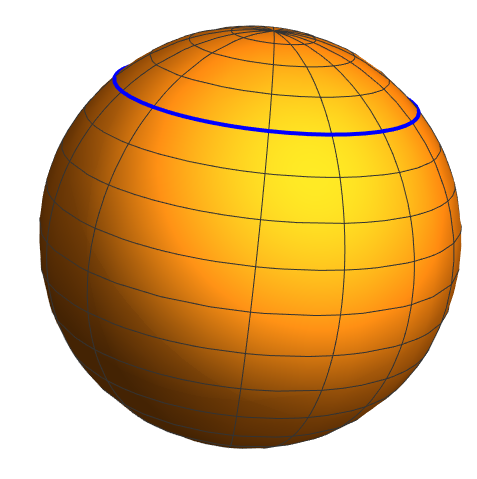
\includegraphics[width=0.4\linewidth]{fig14}
			\label{fig:fig14}
		\end{figure}
		
		Así que tenemos las ecuaciones
		\[\frac{dx}{dt}=-\sen\theta_0\sen t,\qquad\frac{dy}{dt}=\sen\theta_0\cos t,\qquad\frac{dz}{dt}=0\]
		La métrica esférica con estas coordenadas está dada por
		\begin{align*}
			g_{11}=E=\left\langle \frac{\partial}{\partial \theta},\frac{\partial}{\partial \theta}\right\rangle=1,&\qquad g_{22}=G=\left\langle \frac{\partial}{\partial \varphi},\frac{\partial}{\partial \varphi}\right\rangle=\sen^2(\theta)\\
			g_{12}=\left\langle \frac{\partial}{\partial \theta},\frac{\partial}{\partial \varphi}\right\rangle=g_{21}&=\left\langle \frac{\partial}{\partial \varphi},\frac{\partial}{\partial \theta}\right\rangle=F=0,
		\end{align*}
		Y los símbolos de Christoffel son
		\begin{align*}
			\Gamma_{11}^1=\Gamma^2_{11}=\Gamma^2_{12}=\Gamma_{22}^2=0,		\qquad \Gamma_{12}^2=\cot\theta,\qquad\Gamma^1_{22}=-\sen\theta\cos\theta
		\end{align*}
		Definamos un campo vectorial a lo largo de esta curva
		\[W=a(\varphi)\frac{\partial}{\partial\theta}\Big|_{\alpha(\varphi)}+b(\varphi)\frac{\partial}{\partial \varphi}\Big|_{\alpha(\varphi)}\]
		Y tratemos de encontrar las funciones $a$ y $b$ mediante la ecuación
		\[D_{\alpha'}W=0\]
		suponiendo que $W$ es paralelo. Obtenemos
		\begin{align*}
			D_{\frac{\partial}{\partial\varphi}}a(\varphi)\frac{\partial}{\partial\theta}+b(\varphi)\frac{\partial}{\partial\varphi}=0\\
			\implies a'\frac{\partial}{\partial\theta}+aD_{\frac{\partial}{\partial \varphi}}\frac{\partial}{\partial \theta}+b'\frac{\partial}{\partial\varphi}+bD_{\frac{\partial}{\partial \varphi}}\frac{\partial}{\partial\varphi}=0
		\end{align*}
		con condiciones iniciales $a(0)=0$ y $b(0)=1$.
		
		Sustituyendo con los símbolos de Christoffel, obtenemos que
		\begin{align*}
			D_{\frac{\partial}{\partial \varphi}}\frac{\partial}{\partial \theta}&=\cot\theta\frac{\partial}{\partial \varphi}\\
			D_{\frac{\partial}{\partial \varphi}}\frac{\partial}{\partial \varphi}&=-\sen\theta\cos\theta\frac{\partial}{\partial \theta}\\
		\end{align*}
		Así que
		\[a'\frac{\partial}{\partial\theta}+a\cot\theta\frac{\partial}{\partial \varphi}+b'\frac{\partial}{\partial\varphi}-b\sen\theta\cos\theta\frac{\partial}{\partial \theta}=0\]
		Y nuestro problema se reduce a solucionar el sistema
		\[\begin{cases}
			a'-b\sen\theta_0\cos\theta_0=0\\
			b'+a\cot\theta_0=0
		\end{cases}\]
		fijando $\theta_0$ por tratarse de un parelelo, por lo que las funciones $a$ y $b$ dependen de $\varphi$. Derivando respecto a $\varphi$ y sustituyendo obtenemos
		\begin{align*}
			b''+a'\cot\theta_0=0\\
			b''+b\sen\theta_0\cos\theta_0\frac{\cos\theta_0}{\sen\theta_0}=0\\
			b''+b\cos^2\theta_0=0
		\end{align*}
		Que es un oscilador armónico, cuya solución es
		\begin{align*}
			b(\varphi)=\cos(\cos\theta_0\varphi)
		\end{align*}
		Y al sustituir para $a$ obtenemos
		\begin{align*}
			a'=\cos(\cos\theta_0\varphi)\sen\theta_0\cos\theta_0\\
			a(\varphi)=\sen\theta_0\sen(\varphi\cos\theta_0)
		\end{align*}
		
		\begin{figure}[H]
			\begin{center}
				\begin{subfigure}[t]{0.4\linewidth}
					\centering
					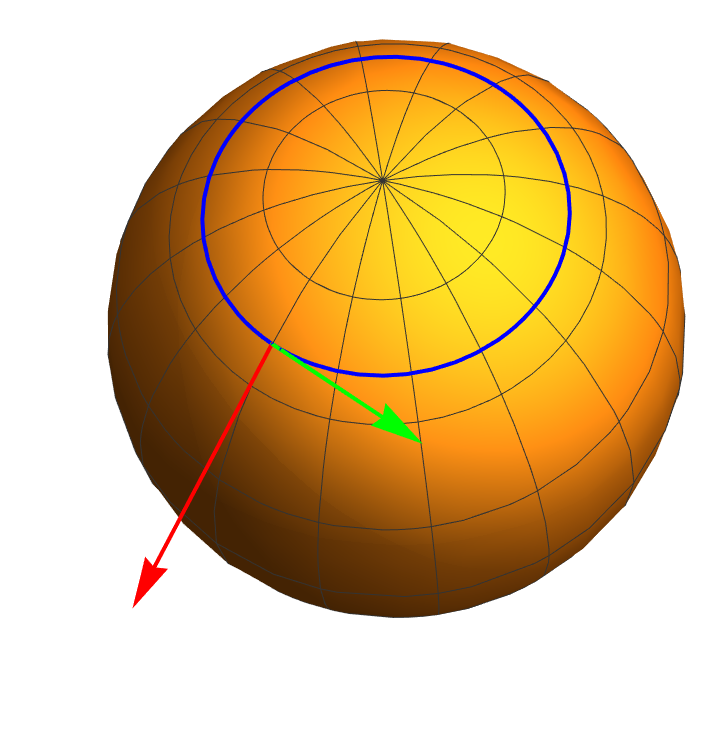
\includegraphics[width=\linewidth]{fig15a}
					\caption*{$\varphi=0$}
				\end{subfigure}
				\begin{subfigure}[t]{0.4\linewidth}
					\centering
					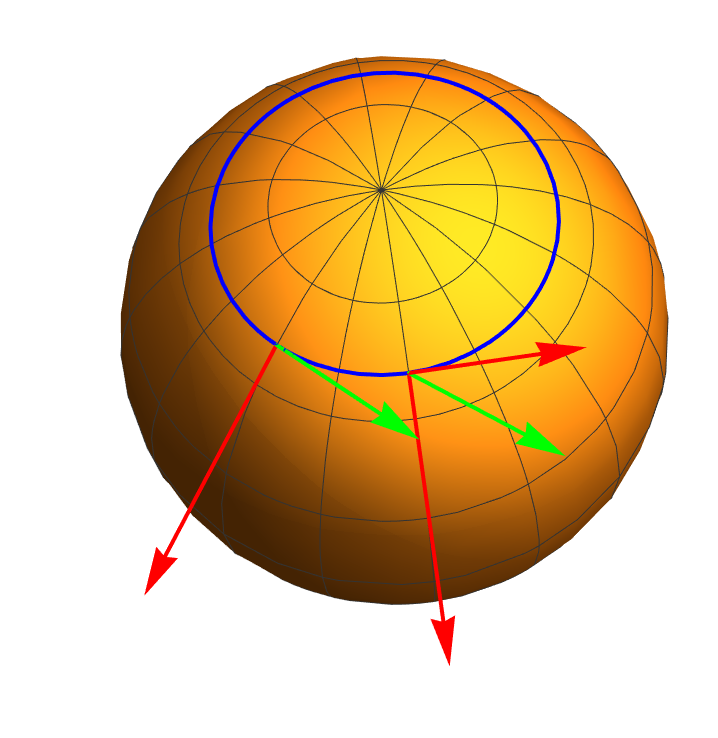
\includegraphics[width=\linewidth]{fig15b}
					\caption*{$\varphi=2\pi/8$}
				\end{subfigure}
				\begin{subfigure}[t]{0.4\linewidth}
					\centering
					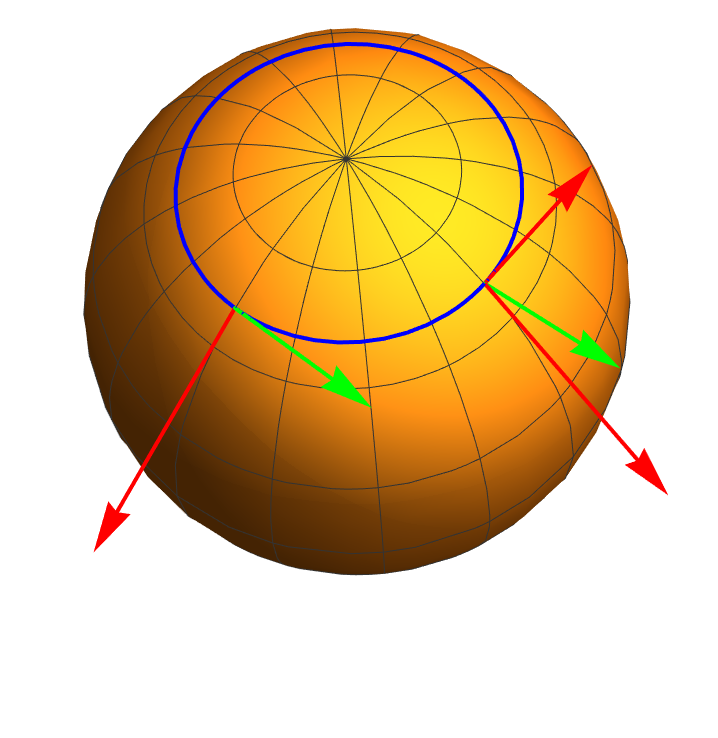
\includegraphics[width=\linewidth]{fig15c}
					\caption*{$\varphi=2\pi/4$}
				\end{subfigure}
				\begin{subfigure}[t]{0.4\linewidth}
					\centering
					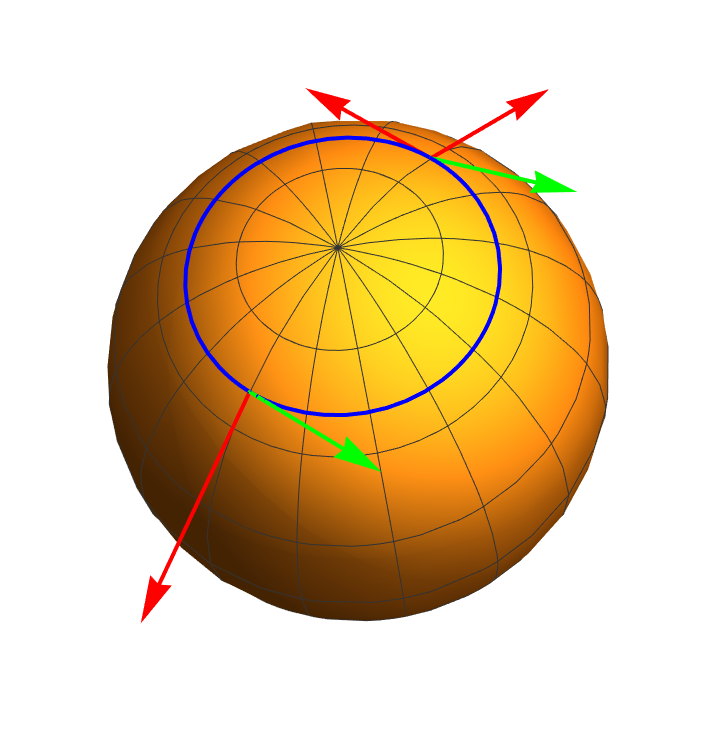
\includegraphics[width=\linewidth]{fig15d}
					\caption*{$\varphi=\pi$}
				\end{subfigure}
				\begin{subfigure}[t]{0.4\linewidth}
					\centering
					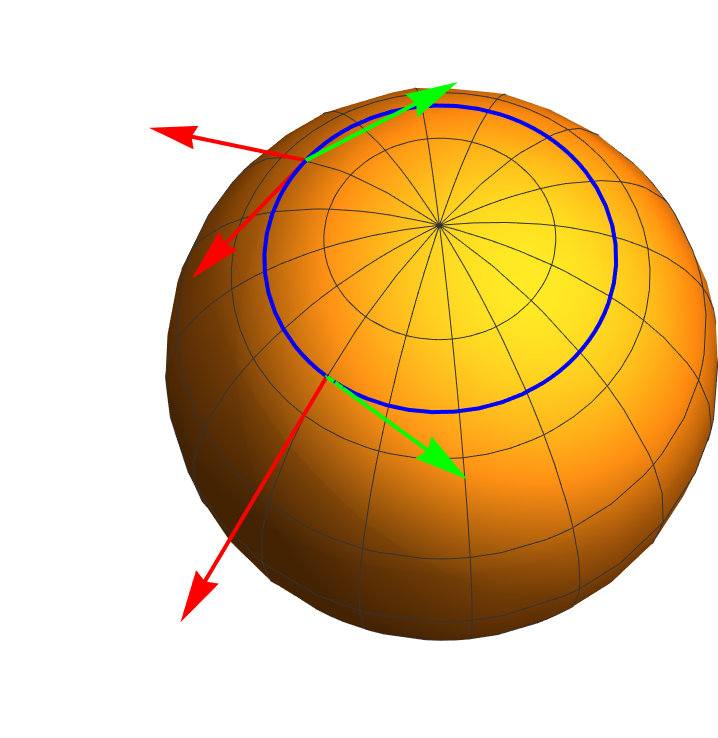
\includegraphics[width=\linewidth]{fig15e}
					\caption*{$\varphi=3\pi/2$}
				\end{subfigure}
				\begin{subfigure}[t]{0.4\linewidth}
					\centering
					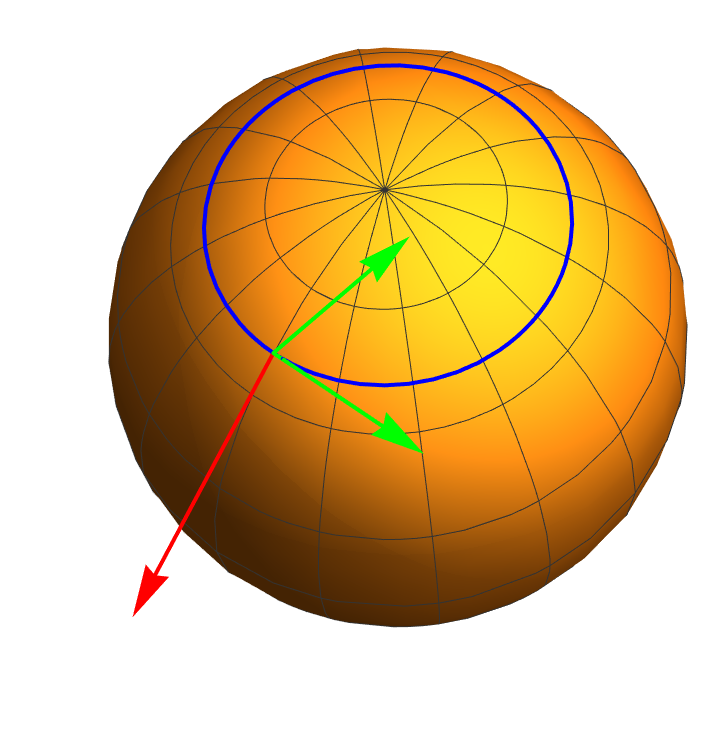
\includegraphics[width=\linewidth]{fig15f}
					\caption*{$\varphi=2\pi$}
				\end{subfigure}
			\end{center}
			\caption*{El transporte paralelo de $W$ (verde) a lo largo del paralelo con $\theta=\pi/5$. Los vectores en rojo son la base canónica.}
		\end{figure}
	\end{ejem}
	
	\begin{ejem}[Transporte paralelo en $S^2$ usando el cono tangente]
		También es posible calcular el transporte paralelo a lo largo de este paralalo usando una isometría local con el cono tangente a la esfera a lo largo de la curva. Una demostración muy detallada está en \href{https://github.com/dan-gc/curvas-superficies/blob/main/curvas-superficies.pdf}{\texttt{curvas-superficies.pdf}}, pág. 51.
		\begin{figure}[H]
			\begin{center}
				\centering
				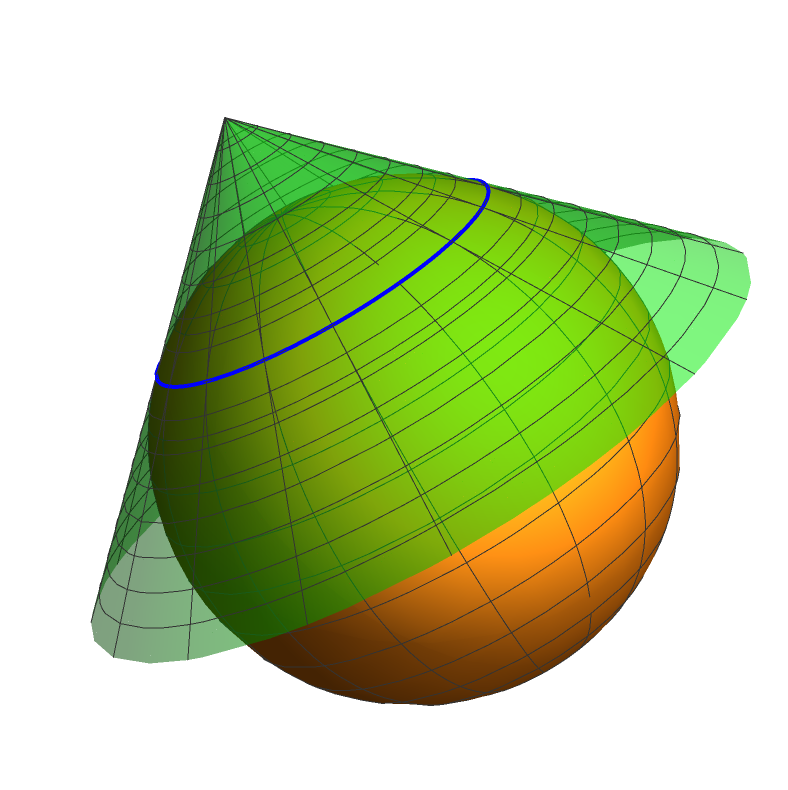
\includegraphics[width=0.5\linewidth]{fig16}
			\end{center}
		\end{figure}
	\end{ejem}
	
	Ahora tratemos de encontrar una ecuación general para describir esta situación:
	\begin{align*}
		D_{\frac{d x^1}{dt}\frac{\partial}{\partial x^1}+\frac{d x^2}{d t}\frac{\partial}{\partial x^2}}W=0\\
		\frac{d x^1}{dt}D_{\frac{\partial}{\partial x^1}}W+\frac{dx^2}{dt}D_{\frac{\partial}{\partial x^2}}W=0
	\end{align*}
	Luego
	\begin{align*}
		\frac{dx^1}{dt}D_{\frac{\partial}{\partial x^1}}\left(a_1\frac{\partial}{\partial x^1}+a_2\frac{\partial}{\partial x^2}\right)+\frac{dx^2}{dt}D_{\frac{\partial}{\partial x^2}}\left(a_1\frac{\partial}{\partial x^1}+a_2\frac{\partial}{\partial x^2}\right)=&0\\
		\implies \frac{dx^1}{dt}\left(\frac{\partial a_1}{\partial x^1}\frac{\partial}{\partial x^1}+a_1D_{\frac{\partial}{\partial x^1}}D\frac{\partial}{\partial x^1}+
		\frac{\partial a_2}{\partial x^1}\frac{\partial}{\partial x^2}+a_2D_{\frac{\partial}{\partial x^1}}D\frac{\partial}{\partial x^2}\right)\\
		+ \frac{dx^2}{dt}\left(\frac{\partial a_1}{\partial x^1}\frac{\partial}{\partial x^1}+a_1D_{\frac{\partial}{\partial x^1}}D\frac{\partial}{\partial x^1}+
		\frac{\partial a_2}{\partial x^1}\frac{\partial}{\partial x^2}+a_2D_{\frac{\partial}{\partial x^1}}D\frac{\partial}{\partial x^2}\right)&=0
	\end{align*}
	
	\begin{defn}
		Dado un vector $W_0\in T_pM$ a lo largo de una curva $\gamma$ en una variedad $M$ con $\gamma(t_0)=p$, el vector en $W_1\in T_qM$ que se obtiene al recorrer la curva $\gamma$ hasta el punto $\gamma(t_1)=q$ se llama \textbf{transporte paralelo de $W_0$}.
	\end{defn}
	
	\begin{prop}[\cite{Loring-dif}\textbf{, prop. 14.6}]
		Si $M$ es Riemanniana, transporte paralelo preserva el producto interno en el sentido de que si $V_0,W_0\in T_pM$, entonces $\langle V_0,W_0\rangle=\langle V_1,W_1\rangle$ con la notación de la definición anterior.
	\end{prop}
	\begin{proof}
		Por la compatibilidad de la métrica Riemanniana
		\[\frac{d}{dt}\left\langle V(t),W(t)\right\rangle=\left\langle \frac{DV}{dt},W\right\rangle+\left\langle V,\frac{DW}{dt}\right\rangle=0\]
		ya que $V$ y $W$ son paralelos.
	\end{proof}
	
	\subsection{Ejercicios 20 de octubre}
	Con la métrica en el semiplano superior dada por $g_{11}=g_{22}=\frac{1}{y^2}$ y $g_{12}=0$,
	\begin{enumerate}
		\item Encuentra los símbolos de Christoffel.
		\item Sea $v_0=(0,1)$ un vector tangente al punto $(0,1)\in\Hy^2$, considera el transporte paralelo $v(t)$ a lo largo de la curva $x=t$, $y=1$. Muestra que el ángulo entre $v(t)$ y la dirección vertical en sentido de las manecillas del reloj es $t$.
	\end{enumerate}
	\begin{proof}[Solución]\leavevmode
		\begin{enumerate}
			\item Con cuentas análogas a \hyperref[ejem:chsitorffel-hip]{las que hicimos antes} obtenemos que
			\[\Gamma^1_{11}=\Gamma^2_{12}=\Gamma^1_{22}=0,\qquad \Gamma_{11}^2=\frac{1}{y},\qquad \Gamma_{22}^2=\Gamma^1_{12}=-\frac{1}{y}\]
			%			\item Tenemos las ecuaciones
			%			\begin{align*}
				%				\frac{da}{dt}-\frac{b}{y}=0\qquad
				%				\frac{db}{dt}+\frac{a}{y}=0
				%			\end{align*}
			%			que en nuestra curva se traducen a
			%			\begin{align*}
				%				\frac{da}{dt}-b=0\qquad
				%				\frac{db}{dt}+a=0
				%			\end{align*}
			%			Tomando
			%			\[a=\sen(\theta(t))\qquad b=\cos(\theta(t))\]
			%			obtenemos
			%			\[a'=\cos(\theta(t))\theta'(t)\qquad b'=-\sen(\theta(t))\theta'(t)\]
			%			y con $\theta=t$ tenemos la solución.
		\end{enumerate}
	\end{proof}
	
	\section{Geodésicas}
	En la sección anterior definimos una curva $\gamma:I\to M$ como geodésica si su campo de velocidades $\gamma'\in\X(\gamma)$ es paralelo, es decir, si $\frac{d\gamma'}{dt}=0$.
	
	Suponiendo que las coordenadas de $\gamma$ son $h\circ\gamma(t)=x^1(t),\ldots,x^n(t)$ para alguna carta coordenada $h$, podemos el campo de velocidades como
	\[\gamma'=\sum_{i=1}^n\frac{dx^i}{dt}\frac{\partial}{\partial x^i}\]
	y la condición de ser geodésica como
	\begin{gather*}
		\frac{d^2x^1}{dt^2}+\sum_{i,j=1}^n\Gamma_{ij}^1\frac{dx^i}{dt}\frac{dx^j}{dt}=0\\
		\vdots\\
		\frac{d^2x^n}{dt^2}+\sum_{i,j=1}^n\Gamma_{ij}^n\frac{dx^i}{dt}\frac{dx^j}{dt}=0
	\end{gather*}
	Introduciendo las variables
	\begin{gather*}
		\frac{dx^1}{dt}=y^1,\qquad	\ldots \qquad
		\frac{dx^n}{dt}=y^n
	\end{gather*}
	Obtenemos el sistema
	\begin{gather*}
		\frac{dy^1}{dt}+\sum\Gamma_{ij}^1y^iy^j=0\\
		\vdots\\
		\frac{dy^n}{dt}+\sum\Gamma_{ij}^ny^iy^j=0
	\end{gather*}
	De hecho podemos considerar la curva $\tilde{\gamma}(t)=\gamma'(t)$ en el haz tangente $TM$,
	\[\begin{tikzcd}
		I\arrow{r}{\tilde{\gamma}}\arrow[swap]{rd}{\tilde{h}\circ\tilde{\gamma}}& TM\arrow{d}{\tilde{h}}\\
		&\R^{2n}		
	\end{tikzcd}\]
	que dará lugar al \textbf{\textit{flujo geodésico}}.
	
	\begin{ejem}
		En el plano hiperbólico $\Hy^2$ con símbolos de Christoffel
		\[\Gamma^1_{11}=\Gamma^2_{12}=\Gamma^1_{22}=0,\qquad \Gamma_{11}^2=\frac{1}{y},\qquad \Gamma_{22}^2=\Gamma^1_{12}=-\frac{1}{y}\]
		obtenemos las ecuaciones
		\begin{align*}
			\frac{d^2x}{dt^2}+\Gamma_{12}^1\frac{dx}{dt}\frac{dy}{dt}+\Gamma^1_{21}\frac{dy}{dt}\frac{dx}{dt}=0\\
			\frac{d^2y}{dt^2}+\Gamma_{11}^2\frac{dx}{dt}\frac{dx}{dt}+\Gamma^2_{22}\frac{dy}{dt}\frac{dy}{dt}=0
		\end{align*}
		y sustituyendo
		\begin{align*}
			\frac{d^2x}{dt^2}-2\frac{1}{y}\frac{dx}{dt}\frac{dy}{dt}&=0\\
			\frac{d^2y}{dt^2}+\frac{1}{y}\left(\frac{dx}{dt}\right)^2-\frac{1}{y}\left(\frac{dy}{dt}\right)^2&=0
		\end{align*}
		Ahora si una curva $\gamma(t)=(x(t),y(t))$ es geodésica y $x(t)=0$, tenemos 
		\[\frac{d^2y}{dt^2}-\frac{1}{y}\left(\frac{dy}{dt}\right)^2=0\]
		cuya solución es, de hecho, $y(t)=e^t$. Para verlo simplemente notemos que en este caso $\left(\frac{dy}{dt}\right)^2=e^{2t}$ y luego $\frac{1}{y}\left(\frac{dy}{dt}\right)^2=e^t$. Entonces, $\gamma$ es una curva vertical recorrida a velocidad exponencial, $\gamma(t)=(0,e^t)$.
		
		\[\begin{tikzpicture}
			% Axes
			\draw[->] (-3,0) -- (3,0) node[right] {};
			\draw[->] (0,-2) -- (0,3) node[above] {};
			
			% Function plot
			\draw[blue, very thick, domain=0:2.8] plot (0,\x);
		\end{tikzpicture}\]
	\end{ejem}
	
	\begin{ejer*}[Geodésicas en una superficie de revolución] Este ejercicio corresponde al ejemplo 5 del capítulo 4.4 del \cite{DoCarmo-sup} de curvas y superficies. También fue desarrollado en \href{https://github.com/dan-gc/curvas-superficies/blob/main/curvas-superficies.pdf}{\texttt{curvas-superficies.pdf}} p. 54. %\href{https://github.com/dan-gc/geo-riem/blob/main/geo-sup-rev.nb}{\texttt{geo-sup-rev.nb}}
		\begin{figure}[H]
			\begin{center}
				\centering
				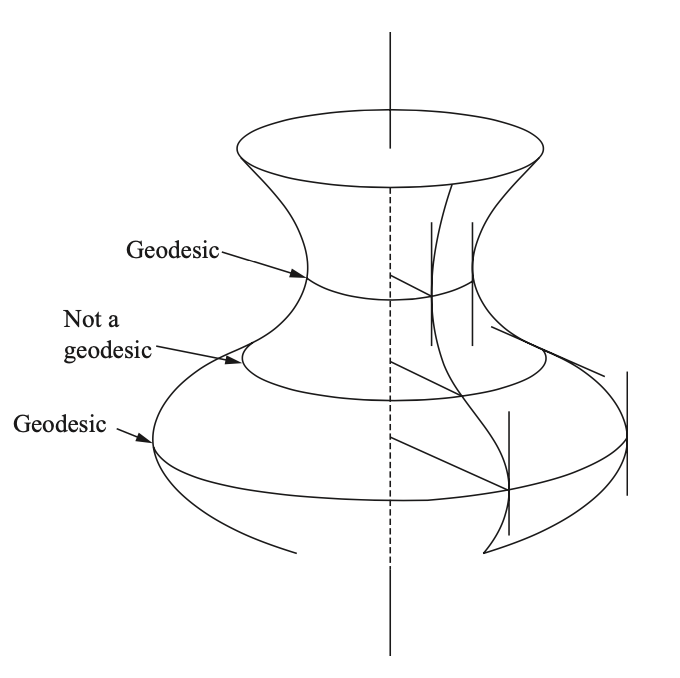
\includegraphics[width=0.5\linewidth]{fig17}
			\end{center}
		\end{figure}
	\end{ejer*}	
	
	\section{La aplicación exponencial}
	Queremos generalizar la siguiente idea:
	
	\begin{figure}[H]
		\centering
		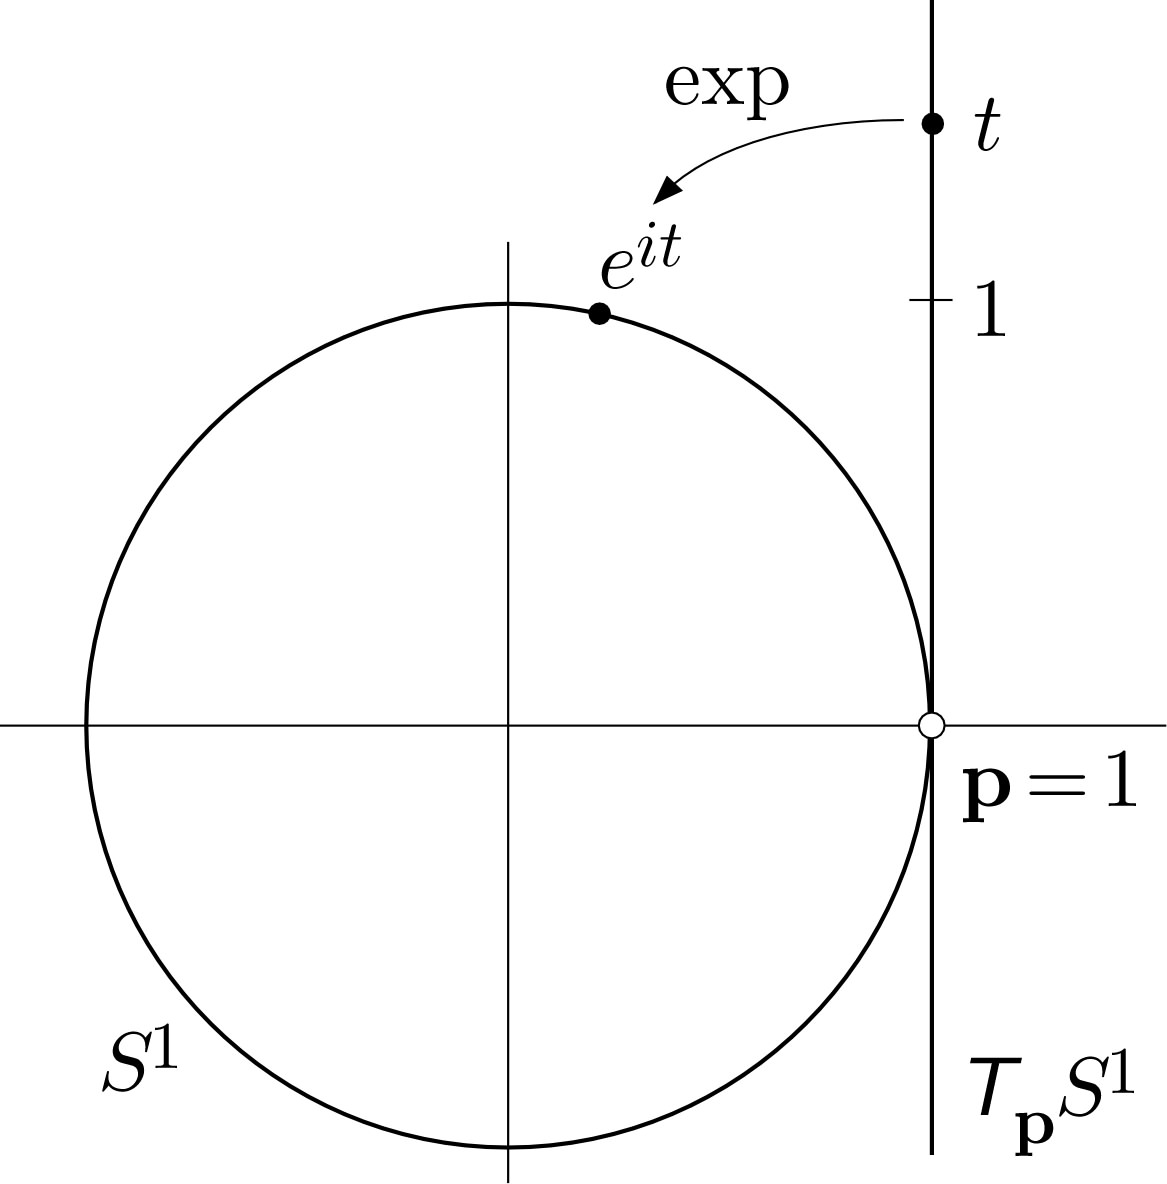
\includegraphics[width=0.4\linewidth]{fig18}
	\end{figure}
	El chiste es que el espacio tangente en un punto nos da un parámetro para desplazarnos sobre la variedad:
	
	\begin{figure}[H]
		\centering
		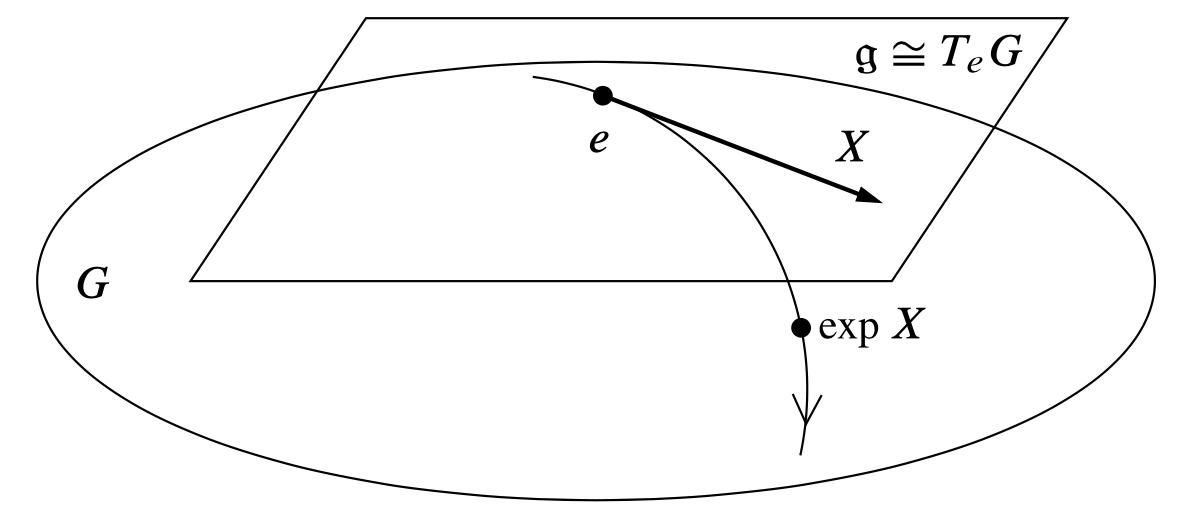
\includegraphics[width=0.5\linewidth]{fig19}
		\caption*{(Imagen de \cite{Lee} donde la variedad es un grupo de Lie.)
			%En este caso se toma el espacio tangente a la identidad, y el espacio tangente es un álgebra de Lie. (En este curso no veremos más sobre esta construcción)
		}
	\end{figure}
	Nos gustaría definir algo así:
	\begin{align*}
		\exp_p:T_pM&\to M\\
		v&\mapsto \gamma(1)
	\end{align*}
	donde $\gamma$ es la única geodésica que pasa por $p$ con velocidad $v$ (que existe por ser la solución de una ecuación diferencial). Pero, ¿está bien definida? La respuesta es que no siempre. Por ejemplo, si la variedad es un cono menos su vértice y tomamos un vector en la dirección de un meridiano muy cerca del vértice, es posible que la geodésica no esté definida en 1.
	
	Para definir correctamente la exponencial debemos restringir el dominio dentro del espacio tangente. El truco es tomar una vecindad muy pequeña cerca del origen para que los vectores tengan magnitud pequeña, así las geodésicas pasarán por el punto a velocidad muy pequeña y cuando las evaluemos en 1 no se habrán ido muy lejos.
	
	\textit{Las referencias a \cite{DoCarmo} que usaremos en esta sección corresponden al capítulo III.}
	
	\begin{prop}[Teos. 2.7 \cite{DoCarmo} y 14.8 \cite{Loring-dif}]
		Dado $p\in M$, existe una vecindad $U$ de $p$ en $M$ y un número $\varepsilon>0$ tal que para cualquier $q\in U$ y $v\in T_qM$ con $|v|<\varepsilon$ hay una única geodésica $\gamma:(-2,2)\to M$ con $\gamma(0)=q$ y $\gamma'(0)=v$.
	\end{prop}
	De hecho, la demostración de esta proposición ya casi está. Por el teorema de existencia y unicidad de ecuaciones diferenciales, sabemos que existen estas geodésicas definidas en algún intervalo, digamos $\gamma:(-\delta,\delta)\to M$ para algún $\delta>0$. Sólo debemos reajustar el dominio, para lo cual usaremos el siguiente lema:
	
	\begin{lema}[De homogeneidad de geodésicas. Lema 2.6 \cite{DoCarmo}, Coro. 14.6 \cite{Loring-dif}]
		Sea $a\in\R$. Si una geodésica $\gamma_v:(-\delta,\delta)\to M$ tiene punto inicial $q$ y velocidad inicial $v$, entonces la curva
		\[\gamma_{av}(t)=\gamma(at)\]
		es una geodésica $\gamma_{av}:(-\frac{\delta}{a},\frac{\delta}{a})\to M$ con punto inicial $q$ y velocidad inicial $av$.
	\end{lema}
	\begin{proof}
		Es claro que $\gamma_{av}(0)=q$ y $\gamma_{av}'(0)=a\gamma_v'(t)=av$. Para ver que es una godésica hacemos
		\[\frac{D}{dt}\frac{d\gamma_v}{dt}=D_{{\gamma_{av}'}(t)}\gamma_{av}'(t)=D_{a\gamma_v'(t)}a\gamma_v'(t)=a^2D_{\gamma'(t)}\gamma_v'(t)=0\]
	\end{proof}
	
	Así que la demostración de la proposición anterior queda así: como (por ecuaciones diferenciales) para vectores $|v|<\hat{\varepsilon}$ hay geodésicas $\gamma_v:(-\delta,\delta)\to M$ que inician en $q$ con velocidad inicial $v$, entonces la geodésica $\gamma_{(\delta/2)v}(t)=(\delta/2t)$ está bien definida para vectores con $|v|<\varepsilon:=\hat{\varepsilon}\delta/2$.
	
	Ahora sí,
	\begin{align*}
		\exp_p:B_{\varepsilon}(0)\subset T_pM&\to M\\
		v&\mapsto \gamma(1)
	\end{align*}
	donde $\gamma=\gamma_{(\delta/2)v}$ como arriba.
	\begin{obs}
		Do Carmo hace la construcción directamente en el haz tangente $TM$, de manera que la exponencial está definida en una vecindad $\mathcal{U}\subset TM$ que son las bolas de radio $<\varepsilon$ en el espacio tangente de puntos $q\in U$ para alguna vecindad de $p$. Para un campo vectorial en $U$ con vectores de tamaño $<\varepsilon$, esta construcción es justamente lo que llamamos \textbf{\textit{flujo geodésico}}.
	\end{obs}
	
	Ahora calculamos la diferencial de esta aplicación. Recordemos que los vectores tangentes en un punto $p$ de una variedad se pueden definir como velocidades de curvas, es decir, son los operadores $f\mapsto \frac{d}{dt}\big|_0f\circ\alpha:=\alpha'(0)f$ para $f\in\Cinf(M,\R)$ y $\alpha:I\to M$ una curva suave que pasa por $p$ en el tiempo 0. En este sentido la diferencial de una función suave $\varphi:M\to N$ manda $v\mapsto (\varphi\circ\alpha)'(0)$ para una curva tal que $\alpha'(0)=v$.
	
	\begin{prop}
		Identificando $T_pM\approx T_0(T_pM)$, la diferencial de la exponencial en el origen del espacio tangente es la identidad $\Id:T_pM\to T_pM$.
	\end{prop}
	\begin{proof}
		Buscamos una curva cuya velocidad inicial sea $v\in T_pM$ y pase por $0$ en el tiempo $0$. Escogiendo $\alpha(t)=vt$,
		\begin{align*}
			d(\exp_p)_0(v)&=d(\exp_p)_0(\alpha'(0))\\
			&=(\exp_p\circ\alpha)'(0)\\
			&=\frac{d}{dt}\Big|_0\exp_p(\alpha(t))\\
			&=\frac{d}{dt}\Big|_0\exp_p(vt)\\
			&=\frac{d}{dt}\Big|_0\gamma_{vt}(1)\\
			&=\frac{d}{dt}\Big|_0\gamma_v(t)\\
			&=v
		\end{align*}
	\end{proof}
	
	Aplicando el teorema de la función inversa, concluimos que $\exp_p$ es un difeomorfismo local en una vecindad del origen en $T_pM$. De hecho, podemos usar esta función como una carta coordenada. Decimos que la vecindad del punto $p$ dada de esta forma es una \textbf{vecindad normal} o \textbf{bola geodésica}.
	
	\begin{obs}[\cite{Loring-dif}\textbf{, Teo. 15.2, y p. 117}]
		Si $f:M\to N$ es una isometría, el siguiente diagrama conmuta:
		\[\begin{tikzcd}
			V\subset T_pM\arrow{r}{df_p}\arrow[swap]{d}{\exp_p}&U\subset T_{f(p)}N\arrow{d}{\exp_{f(p)}}\\
			\tilde{V}\subset M\arrow[swap]{r}{f}&\tilde{U}\subset N
		\end{tikzcd}\]
		donde todas las vecindades se toman lo suficientemente pequeñas para que las funciones sean biyectivas. Pensando que las exponenciales son cartas coordenadas, vemos que la representación en coordenadas de $f$ es justamente su diferencial. En otras palabras, \textit{cualquier isometría tiene una vecindad donde se ve localmente como una función lineal}.
	\end{obs}
	
	\begin{obs}[2.11, \cite{DoCarmo}]
		Habiendo mostrado que los círculos máximos de la esfera $S^n$ son geodésicas, usando la unicidad de los teoremas anteriores se concluye que éstas son todas las geodésicas.
	\end{obs}
	
	
	Ahora tratemos de estudiar la diferencial de la exponencial cuando la evaluamos en un vector distinto del cero. Se trata de una aplicación entre los espacios tangentes a $p$ y a otro punto $q=\exp_p(v)$ para un vector $v\in T_pM$ fijo.
	
	\begin{figure}[H]
		\centering
		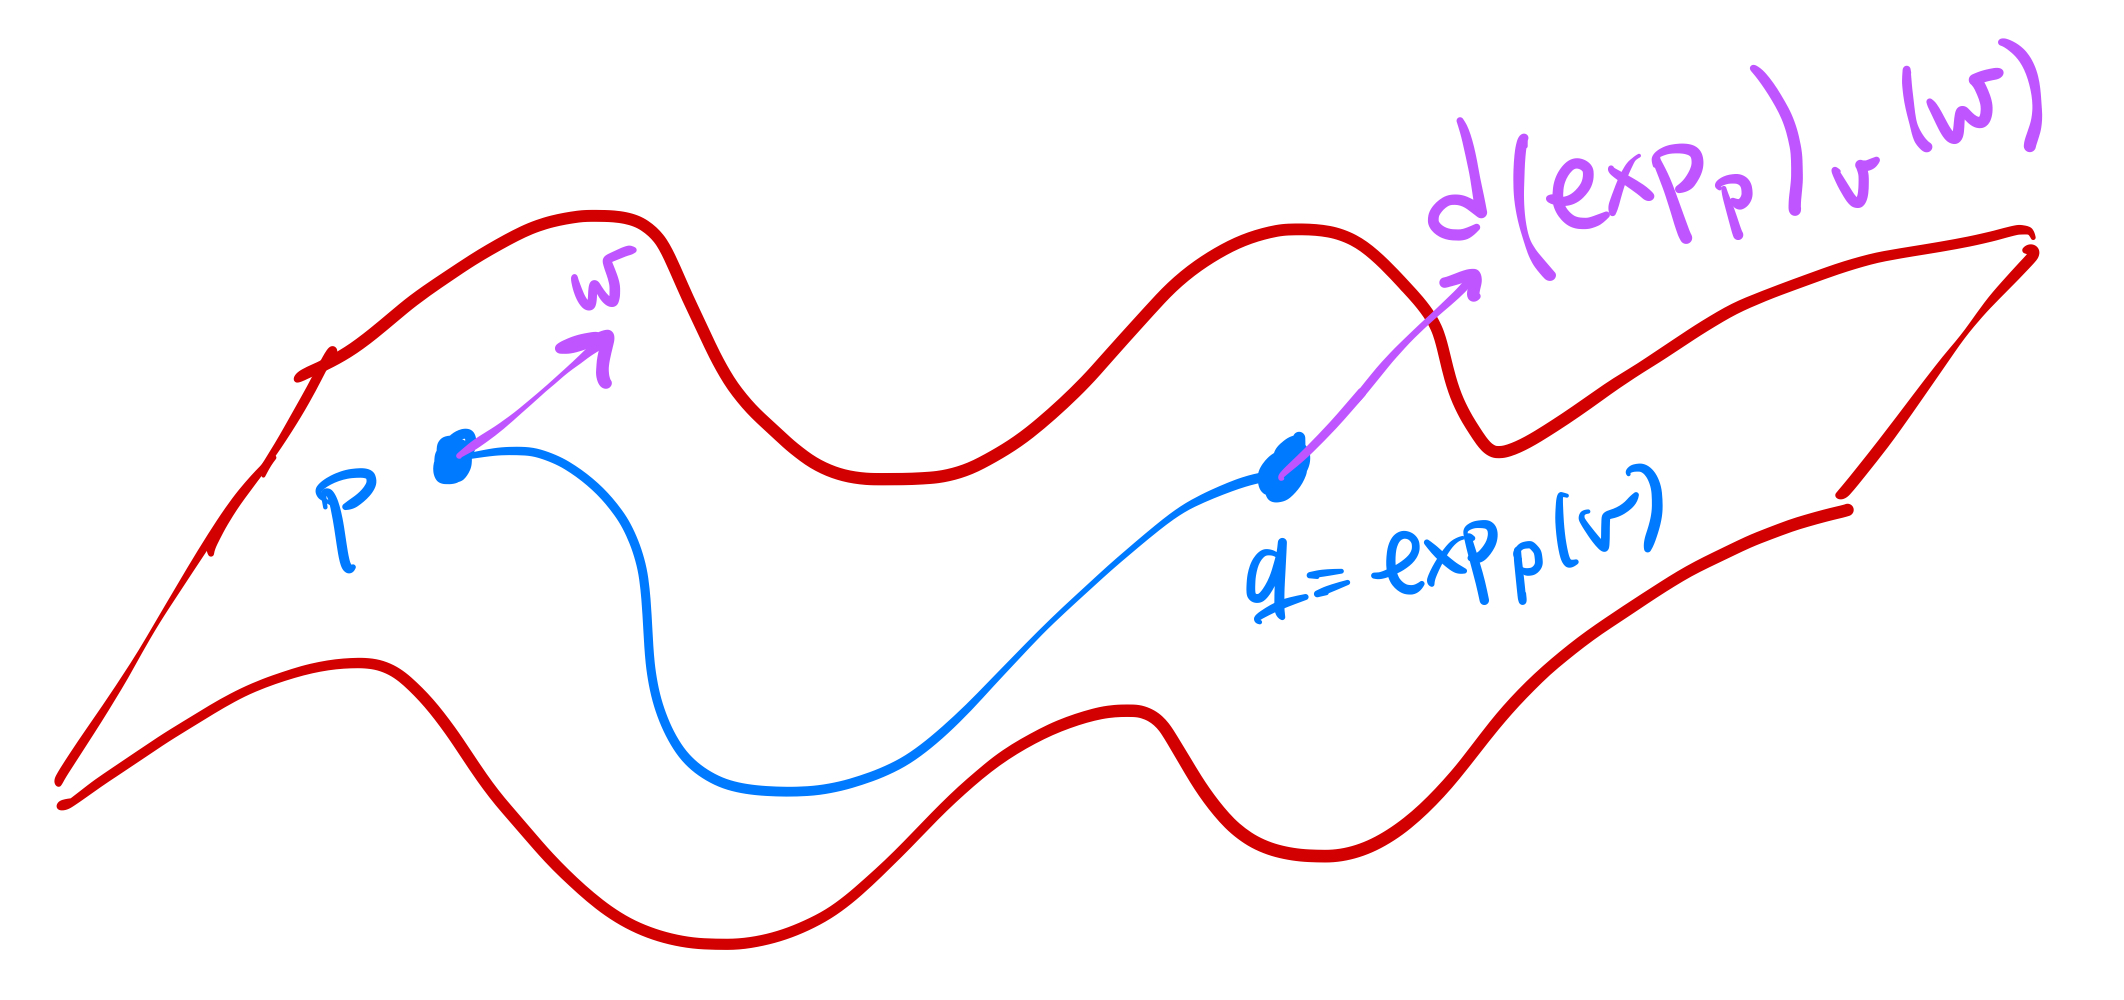
\includegraphics[width=0.7\linewidth]{fig20}
	\end{figure}
	
	En particular, cuando empujamos al mismo vector $v$, obtenemos un vector que sigue siendo tangente a la geodésica. Nos interesa tomar un vector ortogonal a $v$ y ver si al empujarlos siguen siendo ortogonales. Resultará que sí:
	
	%\section{Propiedades minimizantes de las geodésicas}
	
	
	\begin{lema}[de Gauss]
		Sean $p\in M$ y $v\in T_pM$ tales que $\exp_pv$ esté bien definida. Si $w\in T_pM\approx T_v(T_pM)$, entonces
		\[\langle d(\exp_p)_vv,d(\exp_p)_vw\rangle=\langle v,w\rangle\]
	\end{lema}
	
	Que no demostraremos (ver lema 3.5 \cite{DoCarmo}). De hecho, siguiendo a \cite{Lee-riem}, hay otra forma en la que nos interesa enunciar este lema.
	
	\begin{defn}
		Si $U$ es una vecindad normal de $p\in M$, definimos la \textbf{distancia radial} \newline $r:U\to\R$ como
		\[r(x)=\sqrt{(x^1)^2+\ldots+(x^n)^2}\]
		y el \textbf{campo vectorial radial} en $U\backslash \{p\}$ como
		\[\partial_r=\sum_i\frac{x^i}{r(x)}\frac{\partial}{\partial x^i}\]
	\end{defn}
	
	\begin{lema}[de Gauss]
		Sean $(M,g)$ una variedad Riemanniana y $U$ una bola geodésica centrada en $p\in M$. Entonces $\partial_r$ es un campo vectorial unitario ortogonal a la esfera geodésica.
	\end{lema}
	
	Ahora vamos al resultado central de esta sección: las geodésicas minimizan la distancia localmente.
	
	\begin{defn}
		Un segmento de geodésica $\gamma:[a,b]\to M$ es \textbf{minimizante} si $\ell(\gamma)<\ell(\alpha)$ para cualquier curva $\alpha$ diferenciable (por pedazos) que une $\gamma(a)$ con $\gamma(b)$.
	\end{defn}
	
	\begin{prop}[\cite{Lee-riem}\textbf{, 6.11}]
		Sea $(M,g)$ una variedad Riemanniana, $p\in M$ y $B$ una bola geodésica alrededor de $p$. Salvo reparametrizaciones, la geodésica $\gamma:[0,c]\to B$ es la única curva que minimiza la distancia entre $\gamma(0)$ y $\gamma(c)$.
		
		%Supongamos que $p\in M$ y $q$ está contenido en una bola geodésica alrededor de $p$. Entonces (salvo reparametrizaciones) la única geodésica que une $p$ y $q$ es la curva que minimiza la distancia entre $p$ y $q$.
	\end{prop}
	\begin{proof}
		Supongamos que $B=\exp_p(B_\varepsilon(0))$ para algún $\varepsilon>0$, y que la geodésica $\gamma:[0,c]\to B$ tiene velocidad velocidad inicial $v\in T_pM$ y está parametrizada por longitud de arco. Entonces $\ell(\gamma)=c$, y de hecho $\exp_p(tv)=\gamma_{tv}(1)=\gamma_v(t)$. Es decir, en coordenadas normales, la geodésica es una línea.
		
		Ahora tomamos otra curva $\sigma:[0,b]\to M$ también parametrizada por longitud de arco, tal que $\sigma(0)=\gamma(0)$ y $\sigma'(1)=\gamma'(1)$. Restrinjamos el dominio de $\sigma$ a $[a_0,b_0]$ donde $a_0$ es la última vez que pasó por $p$ y $b_0$ es la primera vez después de $a_0$ que tocó la frontera de la bola geodésica.
		
		\begin{figure}[H]
			\centering
			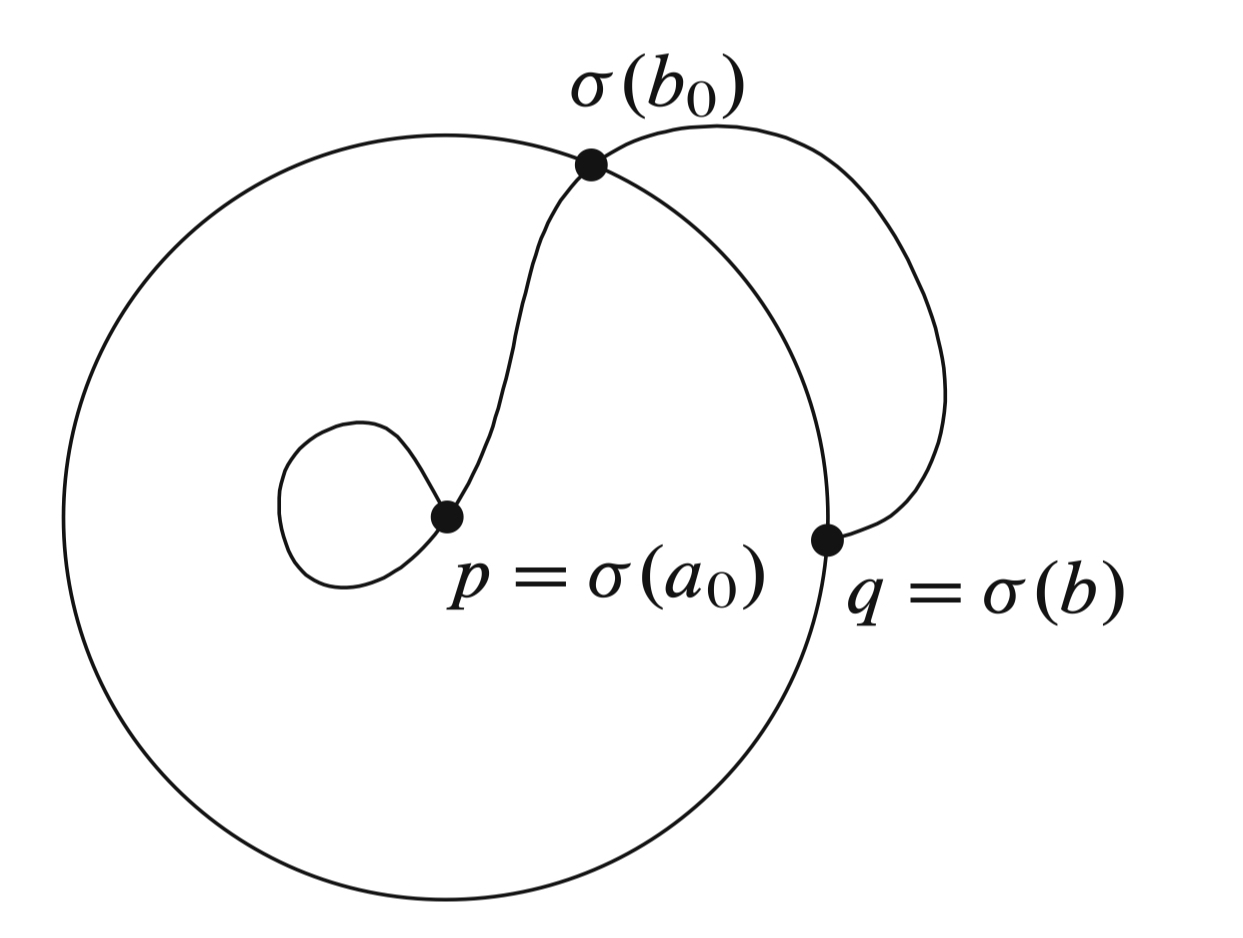
\includegraphics[width=0.4\linewidth]{fig21}
		\end{figure}

		Notemos que el punto $\gamma(c)$ tiene coordenadas $cv$, así que $r(\gamma(c))=|cv|=c$. Además, la función $r\circ\sigma$ es continua en $[a_0,b_0]$ y suave (por pedazos si $\sigma$ es suave por pedazos). Esto nos permite calcular:
		\begin{align*}
			\ell(\gamma)&=c\\
			&=r(\gamma(c))\\
			&=r(\sigma(b_0))-r(\sigma(a_0))\\
			&=\int_{a_0}^{b_0}(r\circ\sigma)' dt\\
			&=\int_{a_0}^{b_0}dr_{\sigma(0)}(\sigma'(t))dt
		\end{align*}
		Nos gustaría que dentro de esta integral apareciera el factor $|\sigma'(t)|$, y así luego encontrar $\ell(\sigma)$. Para esto conviene considerar el \textbf{gradiente} de $r$, el único campo vectorial $\nabla r$ tal que
		\[dr_p(w)=\langle \nabla r,w\rangle\]
		para cualquier $p\in M$ y cualquier $w\in T_pM$ (ver \hyperref[lem:camp-vect-unico]{lema anterior}, \cite{Lee-riem} p.27).
		\begin{af} $\nabla r=\partial_r$.
		\end{af}
		Suponiéndola cierta por ahora podemos seguir con nuestras cuentas:
		\begin{align*}
			\ell(\gamma)&=\int_{a_0}^{b_0}\langle\partial_r,\sigma'(t)\rangle dt\\
			&\leq\int_{a_0}^{b_0}|\partial_r||\sigma'(t)|dt\\
			&=\int_{a_0}^{b_0}|\sigma'(t)|dt\qquad\text{ por el Lema de Gauss, }|\partial_r|=1\\
			&=\ell(\sigma|_{[a_0,b_0]})\leq\ell(\sigma)
		\end{align*}
		Para mostrar unicidad, supongamos que $\ell(\sigma)=c$. Esto obliga a las dos desigualdades en la ecuación anterior a ser igualdades. Como supusimos que ambas curvas están parametrizadas por longitud de arco, $a_0=0$ y $b_0=c$. Además, tendríamos que $\langle \partial_r,\sigma'(t)\rangle=|\partial_r||\sigma'(t)|$ así que estos dos vectores son paralelos y de norma 1, es decir son iguales y las ambas curvas son la solución del mismo sistema de ecuaciones diferenciales.
		

	\end{proof}
	
	La demostración de la afirmación está dada por una caracterización del gradiente como el campo vectorial ortogonal a las curvas de nivel de la función cuya norma es el campo aplicado a la función: aquí es donde entra el lema de Gauss.
	
	\begin{ejer*}[\cite{Lee-riem}\textbf{, 2-10}]
		Sean $(M,g)$ una variedad Riemanniana, $f\in\Cinf(M)$ y $X\in\X(M)$ que no se anula. Entonces, $X=\nabla f$ si y sólo si $Xf=|X|^2$ y $X$ es ortogonal a los conjuntos de nivel de $f$ en todos los puntos regulares.
	\end{ejer*}
	\begin{proof}[Solución]
		\href{https://math.stackexchange.com/questions/4630513/vector-field-that-is-the-gradient-of-a-function-on-riemannian-manifold}{(Ver aquí).} Sólo demostraremos el regreso.
		
		Primero, como $\langle \nabla f, X\rangle=df(X)=Xf$,
		\[|X|^2=\langle X,X\rangle=Xf=\langle\nabla f,X\rangle.\]
		Para usar que $X$ es ortogonal a los conjuntos de nivel tomamos una curva $\alpha:(-\delta,\delta)\to f^{-1}(c)$, cuya velocidad inicial $Y=\alpha'(0)$ es un vector tangente al conjunto de nivel. Luego $f\circ\alpha\equiv c$, así que 
		\[0=(f\circ\alpha)'(0)=df_{\alpha(0)}\alpha'(0)=\langle\nabla f_{\alpha(0)}, \alpha'(0)\rangle\]
		Es decir, el gradiente es ortogonal a los conjuntos de nivel. Como $X$ también,
		\[\nabla f=\lambda X\]
		sustituyendo en la otra ecuación concluimos que $\lambda=1$.
		
	\end{proof}
	
	\begin{proof}
		(de la afirmación) Para ver que $\nabla r=\partial_r$ basta mostrar que $\partial_r$ es ortogonal a los conjuntos de nivel de $r$ (el lema de Gauss) y que $|\partial_r|^2=\partial_rr$. Otra vez por el lema de Gauss $\partial_r$ es unitario, y de hecho
		\[(\partial_r)_xr=\sum_i\frac{x^i}{r(x)}\frac{\partial r}{\partial x^i}\Big|_x=\sum_i\frac{x^i}{r(x)}\frac{1}{2}\frac{2x^i}{r(x)}=1\]
	\end{proof}
	
	Ahora hacemos algunos comentarios mostrando la dirección en la que van estos resultados.
	
	\begin{obs}\leavevmode
		\begin{itemize}
			\item La proposición anterior muestra que dado un punto en la variedad, el segmento de geodésica que pasa por ese punto y llega a otro es minimizante. Falta un poco de trabajo para demostrar que dados cualesquiera dos puntos en una vecindad, existe una geodésica que minimiza la distancia (obs 3.8 \cite{DoCarmo} y teo. 6.15 \cite{Lee-riem}).
			
			\item Esta propiedad no es global: no cualquier arco de geodésica es minimizante. Por ejemplo, un círculo máximo en la esfera que pasa el antípoda no es minimizante.
			
			\item Al revés, la propiedad sí es global: cualquier curva que minimiza la distancia es una geodésica (coro 3.9 \cite{DoCarmo}, p. 167 \cite{Lee-riem}). Esto se demuestra en el contexto de la herramienta usada para primer inciso de esta observación.
		\end{itemize}
	\end{obs}
	
	Un poco más lejos:
	
	\begin{defn}
		Una variedad Riemanniana $M$ es \textbf{completa} si la exponencial está definida en todo el espacio tangente a cada punto. Equivalentemente, las geodésicas que parten de $p\in M$ están definidas en todo $t\in\R$.
	\end{defn}
	
	\begin{teo}[de Hopf-Rinow]
		Una variedad es completa si y sólo si es un espacio métrico completo respecto a la métrica dada por el ínfimo de las longitudes de curvas que unen dos puntos.
	\end{teo}
	
	\begin{coro}[\cite{DoCarmo}\textbf{, Cap VII, 2.9}]
		Si $M$ es compacta entonces es completa.
	\end{coro}
	
	\begin{coro}[\cite{Lee-riem}\textbf{, 6.20}]
		Si $M$ es una variedad Riemanniana conexa y $p\in M$ tal que $\exp_p$ está definida en todo el espacio tangente $T_pM$, entonces $M$ es completa.
	\end{coro}
	\begin{coro}[\cite{Lee-riem}\textbf{, 6.21}]
		Si $M$ es una variedad Riemanniana conexa y completa, cualesquiera dos puntos se pueden unir con una geodésica.
	\end{coro}
	
	Y volviendo a la topología,
	
	\begin{teo}[de Hadamard, \cite{DoCarmo}\textbf{, Cap. VII, 3.1}]
		Si $M$ es completa, simplemente conexa y tiene curvatura seccional $K_p(\sigma)<0$ en todo $p\in M$ y $\sigma\leq T_pM$, entonces es difeomorfa a $\R^n$. Específicamente, $\exp: T_pM\to M$ es un difeomorfismo.
	\end{teo}
	
	\chapter{Curvatura}
	\begin{defn}
		Sea $(M,g)$ una variedad semi-Riemanniana con conexión de Levi-Civita $D$. Definimos el \textbf{tensor de curvatura Riemanniana} como el operador
		\begin{align*}
			R:\X(M)^3&\to\X(M)\\
			(X,Y,Z)&\mapsto R_{XY}Z=D_{[X,Y]}Z-[D_X,D_Y]Z
		\end{align*}
	\end{defn}
	
	\begin{lema}
		El tensor de curvatura puede ser interpretado como un $(1,3$-)campo tensorial, es decir, "saca funciones".
	\end{lema}
	\begin{proof}
		Primero veamos que $R_{XY}fZ=fR_{XY}Z$. Tenemos que
		\begin{align*}
			D_[X,Y]fZ&=([X,Y]f)Z+fD_{[X,Y]}Z\\\\
			-[D_X,D_Y]fZ&=-D_XD_YfZ+D_YD_XfZ\\
			&=-D_X(YfZ+fD_YZ)+D_Y(XfZ+fD_XZ)\\
			&=-XYfZ-YfD_XZ-XfD_YZ-fD_XD_YZ\\
			&\quad+YXfZ+XfD_YZ+YfD_XZfD_YD_XZ
		\end{align*}
		Haciendo la suma se cancelan los términos y obtenemos el resultado.
	\end{proof}
	
	\chapter{Referencias}
	\printbibliography[heading=none]
	
\end{document}